\documentclass[%
 reprint,
 amsmath,amssymb,
 aps,
 prb,
]{revtex4-2}

% Basic packages
\usepackage{graphicx}
\usepackage{bm}

% Float placement control
% \FloatBarrier: prevents floats from drifting past section boundaries
% \usepackage{float} provides [H] specifier for forced inline placement
\usepackage{placeins}
\usepackage{float}

% Quantum mechanics notation
\usepackage{physics}

% Hyperlinks
\usepackage[colorlinks=true,
            linkcolor=blue,
            filecolor=blue,
            urlcolor=blue,
            citecolor=blue]{hyperref}

% Caption settings
\usepackage{caption}
\captionsetup[figure]{
    justification=raggedright,
    labelfont={bf},
    name={Fig.},
    labelsep=period
}
\captionsetup[table]{
    labelfont={bf},
    name={Table},
    labelsep=period
}

% Equation numbering per section
\numberwithin{equation}{section}

% Typographic adjustments
\tolerance=1000
\emergencystretch=1em
\hyphenpenalty=3000
\exhyphenpenalty=3000
\flushbottom

% Microtypography
\usepackage[final]{microtype}
\usepackage{ragged2e}  % for \justifying command

% booktabs for professional tables
\usepackage{booktabs}

% Theorem environment
\usepackage{amsthm}
\newtheorem{theorem}{Theorem}[section]
\newtheorem{lemma}[theorem]{Lemma}
\newtheorem{proposition}[theorem]{Proposition}
\newtheorem{corollary}[theorem]{Corollary}
\theoremstyle{definition}
\newtheorem{definition}{Definition}[section]
\theoremstyle{remark}
\newtheorem{remark}{Remark}[section]

% Code listings with syntax highlighting
\usepackage{listings}
\usepackage{xcolor}

% Color definitions
\definecolor{backcolour}{rgb}{0.96,0.97,0.98}
\definecolor{deepblue}{rgb}{0,0,0.5}
\definecolor{deepgreen}{rgb}{0,0.5,0.3}
\definecolor{deepgray}{rgb}{0.4,0.4,0.4}
\definecolor{stringcolor}{rgb}{0.2,0.4,0.6}

% Python style definition
\lstdefinestyle{pythonstyle}{
    backgroundcolor=\color{backcolour},
    commentstyle=\color{deepgreen}\itshape,
    keywordstyle=\color{deepblue}\bfseries,
    numberstyle=\tiny\color{deepgray},
    stringstyle=\color{stringcolor},
    basicstyle=\ttfamily\footnotesize,
    breakatwhitespace=false,
    breaklines=true,
    captionpos=b,
    keepspaces=true,
    numbers=left,
    numbersep=5pt,
    showspaces=false,
    showstringspaces=false,
    showtabs=false,
    tabsize=2,
    language=Python,
    frame=single,
    rulecolor=\color{deepgray}
}
\lstset{style=pythonstyle}

% TikZ
\usepackage{tikz}
\usetikzlibrary{arrows.meta, calc, 3d, shadings, positioning, decorations.pathmorphing, shapes.geometric}

% Internal phase notation
\newcommand{\iphase}{\theta}  % internal geometric phase = ωt/2

% Custom Macros
\newcommand{\Sphere}{S^0}
\newcommand{\Sone}{S^1}
\newcommand{\Uone}{U(1)}
\newcommand{\lambdaC}{\lambda_{\text{C}}}  % Compton wavelength

% ========================================
% TikZ macro #1 (first citation: fig:three_phases)
% Usage: \figThreePhaseStructures
% ========================================
\newcommand{\figThreePhaseStructures}{%
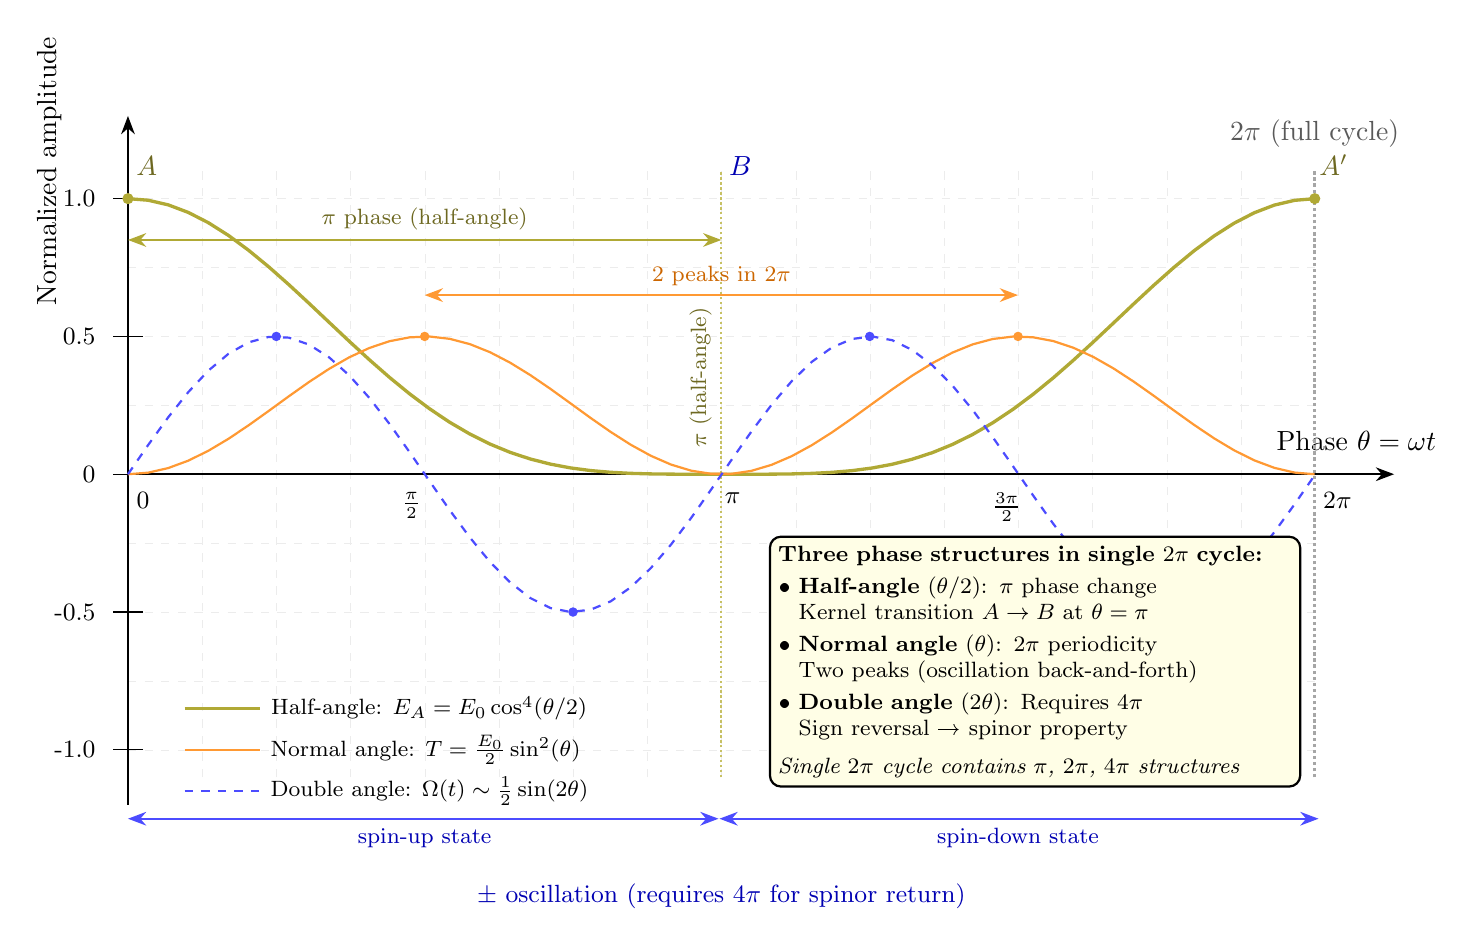
\begin{tikzpicture}[
    x=2.4cm,  % 横幅（0 → 2π の範囲に最適化）
    y=3.5cm,  % 縦幅
    >=Stealth
]
    % --- グリッド ---
    \draw[gray!15, xstep=0.3927, ystep=0.25, dashed, very thin] (0,-1.1) grid (6.28, 1.1);
    
    % --- 座標軸 ---
    \draw[thick, ->] (0,0) -- (6.7,0);
    \draw[thick, ->] (0,-1.2) -- (0,1.3);
    
    % --- 軸ラベル ---
    \node[font=\normalsize, anchor=south] at (6.5, 0.05) {Phase $\theta = \omega t$};
    \node[font=\normalsize, anchor=south, rotate=90] at (-0.3, 1.1) {Normalized amplitude};
    
    % --- 目盛りとラベル（縦軸）---
    \foreach \y in {-1.0, -0.5, 0, 0.5, 1.0} {
        \draw (0.08, \y) -- (-0.08, \y);
        \node[left, font=\small] at (-0.12, \y) {\y};
    }
    
    % --- 目盛りとラベル（横軸）---
    \node[below, font=\small, yshift=-3pt] at (0.08, 0) {$0$};
    \node[below, font=\small, yshift=-3pt] at (1.50, 0) {$\frac{\pi}{2}$};
    \node[below, font=\small, yshift=-3pt] at (3.20, 0) {$\pi$};
    \node[below, font=\small, yshift=-3pt] at (4.65, 0) {$\frac{3\pi}{2}$};
    \node[below, font=\small, yshift=-3pt] at (6.40, 0) {$2\pi$};
    
    % --- 重要な境界線 ---
    % π境界（半角位相の1周期）
    \draw[olive!50, densely dotted, thick] (3.14, -1.1) -- (3.14, 1.1);
    \node[above, font=\footnotesize, olive!70!black, rotate=90, anchor=south] at (3.14, 0.35) {$\pi$ (half-angle)};
    
    % 2π境界（通常角位相の1周期、全体の境界）
    \draw[gray!70, densely dotted, very thick] (6.28, -1.1) -- (6.28, 1.1);
    \node[above, font=\normalsize, gray!70!black] at (6.28, 1.15) {$2\pi$ (full cycle)};
    
    % --- カーネル遷移のマーカー ---
    \node[above, font=\normalsize, olive!70!black] at (0.1, 1.05) {$A$};
    \node[above, font=\normalsize, blue!70!black] at (3.24, 1.05) {$B$};
    \node[above, font=\normalsize, olive!70!black] at (6.38, 1.05) {$A'$};
    
    % --- (1) 半角位相: E_A = cos^4(θ/2) ---
    \draw[olive!70, very thick, domain=0:6.28, samples=60] 
        plot (\x, {(cos(\x * 180 / 3.14159 / 2)^4)});
    \filldraw[olive!70] (0, 1.0) circle (1.8pt);
    \filldraw[olive!70] (6.28, 1.0) circle (1.8pt);
    
    % --- (2) 通常角位相: T = (1/2)sin^2(θ) ---
    \draw[orange!80, thick, domain=0:6.28, samples=60] 
        plot (\x, {0.5*(sin(\x * 180 / 3.14159)^2)});
    \filldraw[orange!80] (1.57, 0.5) circle (1.5pt);
    \filldraw[orange!80] (4.71, 0.5) circle (1.5pt);
    
    % --- (3) 倍角位相: Ω(t) ~ (1/2)sin(2θ) ---
    \draw[blue!70, thick, dashed, domain=0:6.28, samples=60] 
    plot (\x, {0.5*sin(2 * \x * 180 / 3.14159)});
    % Positive peaks
    \filldraw[blue!70] (0.785, 0.5) circle (1.5pt);
    \filldraw[blue!70] (3.925, 0.5) circle (1.5pt);
    % Negative peaks
    \filldraw[blue!70] (2.355, -0.5) circle (1.5pt);
    \filldraw[blue!70] (5.495, -0.5) circle (1.5pt);
    
    % --- アノテーション（3つの位相構造）---
    
    % (1) 半角: π位相変化
    \draw[<->, olive!70, thick] (0, 0.85) -- (3.14, 0.85);
    \node[above, font=\footnotesize, olive!70!black] at (1.57, 0.85) {$\pi$ phase (half-angle)};
    
    % (2) 通常角: 2回ピーク
    \draw[<->, orange!80, thick] (1.57, 0.65) -- (4.71, 0.65);
    \node[above, font=\footnotesize, orange!80!black] at (3.14, 0.65) {2 peaks in $2\pi$};
    
    % (3) 倍角: ±振動
    \draw[<->, blue!70, thick] (0.000, -1.25) -- (3.125, -1.25);
    \node[below, font=\footnotesize, blue!70!black] at (1.57, -1.25) {spin-up state};
    
    \draw[<->, blue!70, thick] (3.130, -1.25) -- (6.3, -1.25);
    \node[below, font=\footnotesize, blue!70!black] at (4.710, -1.25) {spin-down state};
    
    \node[below, font=\small, blue!70!black] at (3.14, -1.45) 
        {$\pm$ oscillation (requires $4\pi$ for spinor return)};
    
    % --- 凡例 ---
    \begin{scope}[shift={(0.3, -0.85)}]
        \draw[olive!70, very thick] (0,0) -- (0.4,0) 
            node[right, font=\footnotesize, black] {Half-angle: $E_A = E_0\cos^4(\theta/2)$};
        \draw[orange!80, thick] (0,-0.15) -- (0.4,-0.15) 
            node[right, font=\footnotesize, black] {Normal angle: $T = \frac{E_0}{2}\sin^2(\theta)$};
        \draw[blue!70, thick, dashed] (0,-0.3) -- (0.4,-0.3) node[right, font=\footnotesize, black] {Double angle: $\Omega(t) \sim \frac{1}{2}\sin(2\theta)$};
    \end{scope}
    
    % --- 説明ボックス ---
    \node[draw, thick, rounded corners, fill=yellow!10, text width=6.5cm, font=\footnotesize, align=left] 
        at (4.8, -0.68) {
        \textbf{Three phase structures in single $2\pi$ cycle:}\\[2pt]
        • \textbf{Half-angle} $(\theta/2)$: $\pi$ phase change\\
        \phantom{•} Kernel transition $A \to B$ at $\theta = \pi$\\[2pt]
        • \textbf{Normal angle} $(\theta)$: $2\pi$ periodicity\\
        \phantom{•} Two peaks (oscillation back-and-forth)\\[2pt]
        • \textbf{Double angle} $(2\theta)$: Requires $4\pi$\\
        \phantom{•} Sign reversal → spinor property\\[4pt]
        \textit{Single $2\pi$ cycle contains $\pi$, $2\pi$, $4\pi$ structures}
    };
    
\end{tikzpicture}%
}

% ========================================
% TikZ macro #2 (second citation: fig:two_spin_schemes)
% Usage: \figTwoSpinSchemes
% ========================================
\newcommand{\figTwoSpinSchemes}{%
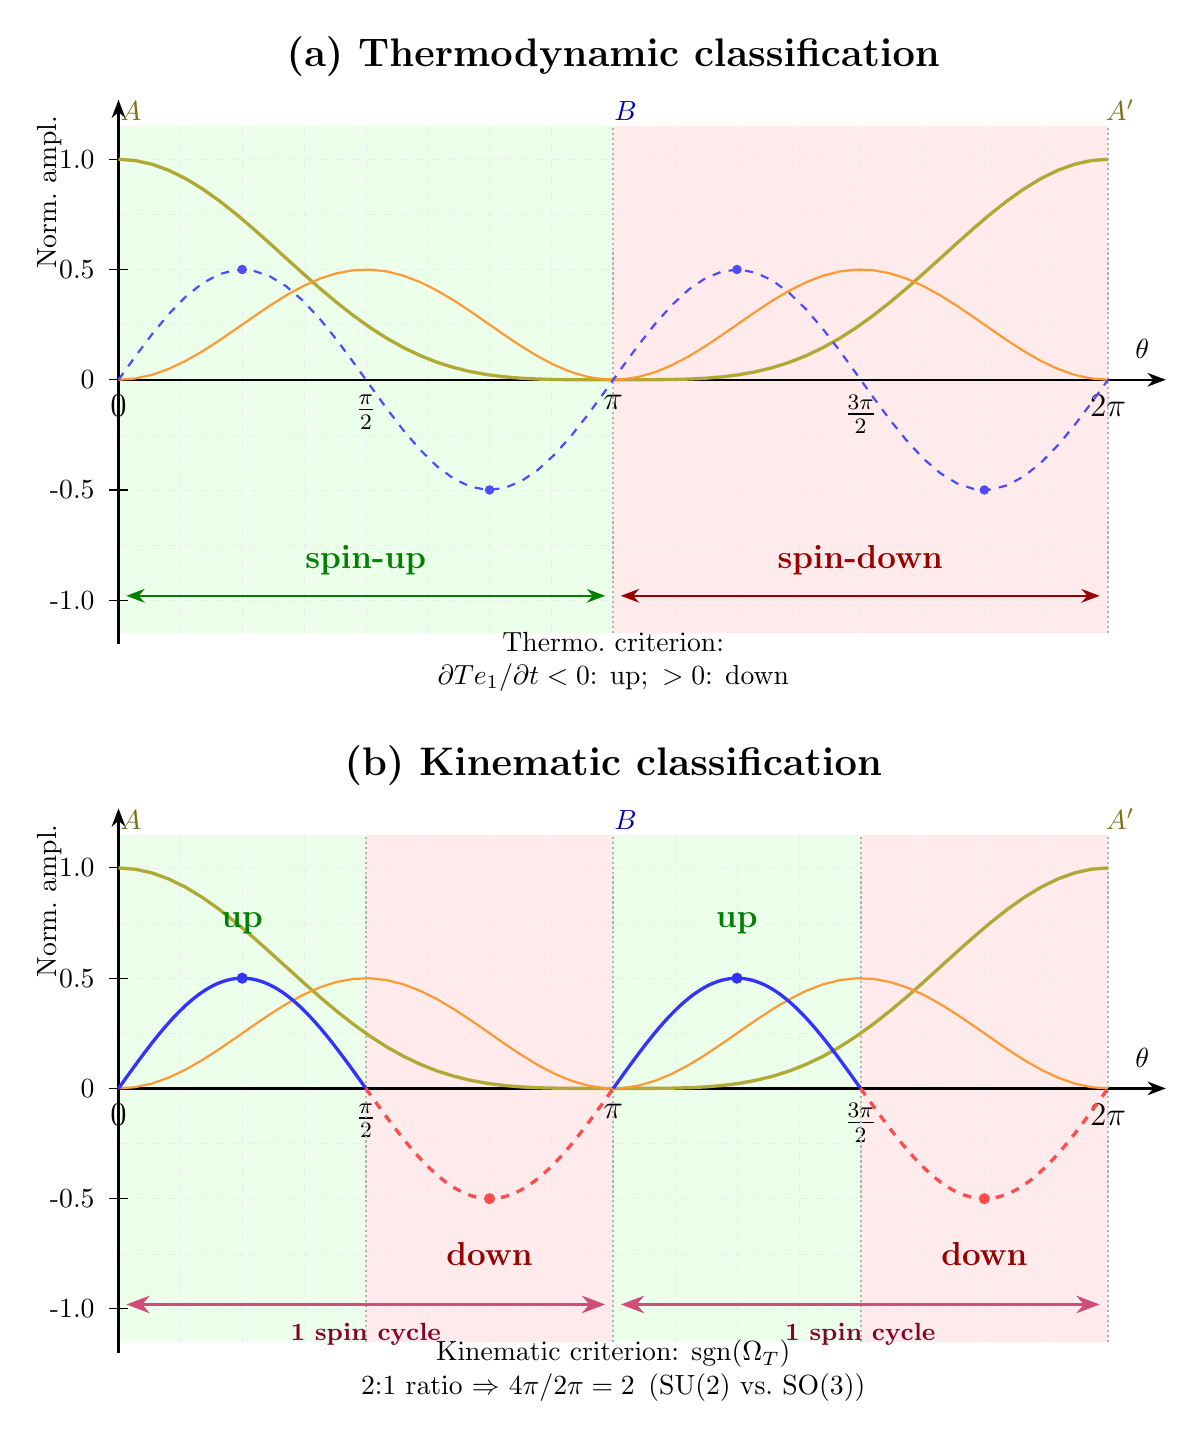
\begin{tikzpicture}[>=Stealth, x=2.0cm, y=2.8cm]

\def\ylo{-1.15}
\def\yhi{1.15}
\def\xmax{6.28318}

% ============================================================
% UPPER PANEL (a): Thermodynamic classification
% ============================================================

\node[font=\Large\bfseries, anchor=south] at (3.14159, \yhi+0.18)
    {(a) Thermodynamic classification};

\fill[green!8] (0,       \ylo) rectangle (3.14159, \yhi);
\fill[red!8]   (3.14159, \ylo) rectangle (\xmax,   \yhi);

\draw[gray!15, xstep=0.3927, ystep=0.25, dashed, very thin]
    (0,\ylo) grid (\xmax, \yhi);
\draw[thick, ->] (0,0) -- (6.65,0);
\draw[thick, ->] (0,\ylo-0.05) -- (0,\yhi+0.12);

\node[font=\normalsize, anchor=south] at (6.5, 0.05) {$\theta$};
\node[font=\normalsize, anchor=south, rotate=90] at (-0.30, 0.85) {Norm.\ ampl.};

\foreach \y in {-1.0, -0.5, 0, 0.5, 1.0} {
    \draw (0.06,\y) -- (-0.06,\y);
    \node[left, font=\normalsize] at (-0.09,\y) {\y};
}
\node[below, font=\large, yshift=-2pt] at (0,       0) {$0$};
\node[below, font=\large, yshift=-2pt] at (1.5708,  0) {$\frac{\pi}{2}$};
\node[below, font=\large, yshift=-2pt] at (3.14159, 0) {$\pi$};
\node[below, font=\large, yshift=-2pt] at (4.7124,  0) {$\frac{3\pi}{2}$};
\node[below, font=\large, yshift=-2pt] at (6.28318, 0) {$2\pi$};

\draw[gray!60, densely dotted, thick] (3.14159,\ylo) -- (3.14159,\yhi);
\draw[gray!60, densely dotted, thick] (6.28318,\ylo) -- (6.28318,\yhi);

\node[font=\normalsize, olive!80!black, above] at (0.08,    \yhi-0.02) {$A$};
\node[font=\normalsize, blue!70!black,  above] at (3.22,    \yhi-0.02) {$B$};
\node[font=\normalsize, olive!80!black, above] at (6.36,    \yhi-0.02) {$A'$};

\draw[olive!70, very thick, domain=0:\xmax, samples=60]
    plot (\x, {(cos(\x * 180 / 3.14159 / 2))^4});
\draw[orange!80, thick, domain=0:\xmax, samples=60]
    plot (\x, {0.5*(sin(\x * 180 / 3.14159))^2});
\draw[blue!70, thick, dashed, domain=0:\xmax, samples=60]
    plot (\x, {0.5*sin(2 * \x * 180 / 3.14159)});

\filldraw[blue!70] (0.7854,  0.5) circle (1.5pt);
\filldraw[blue!70] (2.3562, -0.5) circle (1.5pt);
\filldraw[blue!70] (3.9270,  0.5) circle (1.5pt);
\filldraw[blue!70] (5.4978, -0.5) circle (1.5pt);

\node[font=\large\bfseries, green!50!black] at (1.57, -0.82) {spin-up};
\node[font=\large\bfseries, red!60!black]   at (4.71, -0.82) {spin-down};
\draw[<->, green!50!black, thick] (0.05, -0.98) -- (3.09, -0.98);
\draw[<->, red!60!black,   thick] (3.19, -0.98) -- (6.23, -0.98);

\node[font=\normalsize, align=center] at (3.14159, -1.28)
    {Thermo.\ criterion:\\$\partial Te_1/\partial t < 0$: up;\enspace $> 0$: down};

% ============================================================
% LOWER PANEL (b): Kinematic classification
% ============================================================

\begin{scope}[yshift=-9.0cm]

\node[font=\Large\bfseries, anchor=south] at (3.14159, \yhi+0.18)
    {(b) Kinematic classification};

\fill[green!8]  (0,       \ylo) rectangle (1.5708,  \yhi);
\fill[red!8]    (1.5708,  \ylo) rectangle (3.14159, \yhi);
\fill[green!8]  (3.14159, \ylo) rectangle (4.7124,  \yhi);
\fill[red!8]    (4.7124,  \ylo) rectangle (\xmax,   \yhi);

\draw[gray!15, xstep=0.3927, ystep=0.25, dashed, very thin]
    (0,\ylo) grid (\xmax, \yhi);
\draw[thick, ->] (0,0) -- (6.65,0);
\draw[thick, ->] (0,\ylo-0.05) -- (0,\yhi+0.12);

\node[font=\normalsize, anchor=south] at (6.5, 0.05) {$\theta$};
\node[font=\normalsize, anchor=south, rotate=90] at (-0.30, 0.85) {Norm.\ ampl.};

\foreach \y in {-1.0, -0.5, 0, 0.5, 1.0} {
    \draw (0.06,\y) -- (-0.06,\y);
    \node[left, font=\normalsize] at (-0.09,\y) {\y};
}
\node[below, font=\large, yshift=-2pt] at (0,       0) {$0$};
\node[below, font=\large, yshift=-2pt] at (1.5708,  0) {$\frac{\pi}{2}$};
\node[below, font=\large, yshift=-2pt] at (3.14159, 0) {$\pi$};
\node[below, font=\large, yshift=-2pt] at (4.7124,  0) {$\frac{3\pi}{2}$};
\node[below, font=\large, yshift=-2pt] at (6.28318, 0) {$2\pi$};

\foreach \xb in {1.5708, 3.14159, 4.7124, 6.28318} {
    \draw[gray!60, densely dotted, thick] (\xb, \ylo) -- (\xb, \yhi);
}

\node[font=\normalsize, olive!80!black, above] at (0.08,    \yhi-0.02) {$A$};
\node[font=\normalsize, blue!70!black,  above] at (3.22,    \yhi-0.02) {$B$};
\node[font=\normalsize, olive!80!black, above] at (6.36,    \yhi-0.02) {$A'$};

\draw[olive!70, very thick, domain=0:\xmax, samples=60]
    plot (\x, {(cos(\x * 180 / 3.14159 / 2))^4});
\draw[orange!80, thick, domain=0:\xmax, samples=60]
    plot (\x, {0.5*(sin(\x * 180 / 3.14159))^2});

\draw[blue!80, very thick, domain=0:1.5708, samples=60]
    plot (\x, {0.5*sin(2 * \x * 180 / 3.14159)});
\draw[blue!80, very thick, domain=3.14159:4.7124, samples=60]
    plot (\x, {0.5*sin(2 * \x * 180 / 3.14159)});
\draw[red!70, very thick, dashed, domain=1.5708:3.14159, samples=60]
    plot (\x, {0.5*sin(2 * \x * 180 / 3.14159)});
\draw[red!70, very thick, dashed, domain=4.7124:6.28318, samples=60]
    plot (\x, {0.5*sin(2 * \x * 180 / 3.14159)});

\filldraw[blue!80] (0.7854,  0.5) circle (1.8pt);
\filldraw[red!70]  (2.3562, -0.5) circle (1.8pt);
\filldraw[blue!80] (3.9270,  0.5) circle (1.8pt);
\filldraw[red!70]  (5.4978, -0.5) circle (1.8pt);

\node[font=\large\bfseries, green!50!black] at (0.785,  0.75) {up};
\node[font=\large\bfseries, red!60!black]   at (2.356, -0.75) {down};
\node[font=\large\bfseries, green!50!black] at (3.927,  0.75) {up};
\node[font=\large\bfseries, red!60!black]   at (5.498, -0.75) {down};

\draw[<->, purple!70, very thick] (0.05, -0.98) -- (3.09, -0.98);
\node[font=\small\bfseries, purple!70!black, below] at (1.57, -1.02) {1 spin cycle};
\draw[<->, purple!70, very thick] (3.19, -0.98) -- (6.23, -0.98);
\node[font=\small\bfseries, purple!70!black, below] at (4.71, -1.02) {1 spin cycle};

\node[font=\normalsize, align=center] at (3.14159, -1.28)
    {Kinematic criterion: $\mathrm{sgn}(\Omega_T)$\\
     2:1 ratio $\Rightarrow$ $4\pi/2\pi=2$\enspace (SU(2) vs.\ SO(3))};

\end{scope}

\end{tikzpicture}%
}

% ========================================
% TikZ macro #3 (third citation: fig:bloch_sphere)
% Usage: \figBlochSphere
% ========================================
\newcommand{\figBlochSphere}{%
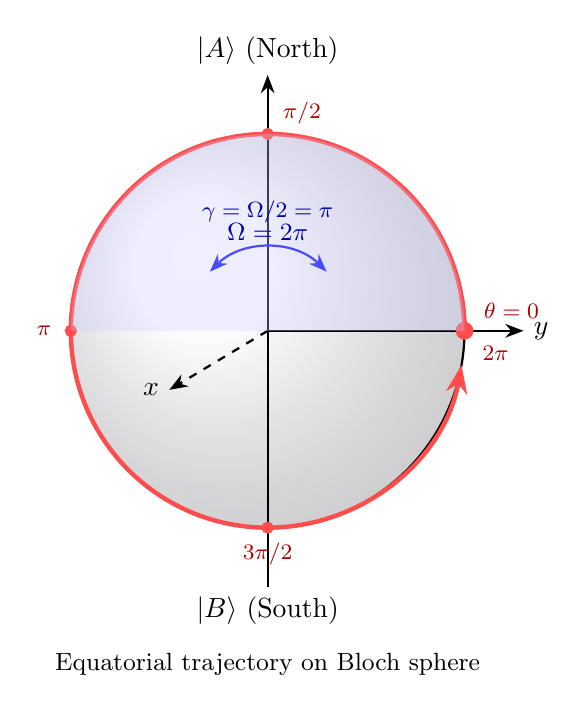
\begin{tikzpicture}[scale=2.5, >=Stealth]
    
    % --- Bloch球の描画 ---
    % 球の輪郭
    \shade[ball color=blue!5, opacity=0.3] (0,0) circle (1cm);
    \draw[thick] (0,0) circle (1cm);
    
    % --- 座標軸 ---
    % z軸（縦）
    \draw[thick, ->] (0,0) -- (0,1.3) node[above] {$|A\rangle$ (North)};
    \draw[thick] (0,0) -- (0,-1.3) node[below] {$|B\rangle$ (South)};
    
    % y軸
    \draw[thick, ->] (0,0) -- (1.3,0) node[right] {$y$};
    
    % x軸（奥行き、破線で表現）
    \draw[thick, dashed, ->] (0,0) -- (-0.5,-0.3) node[left] {$x$};
    
    % --- 赤道（θ: 0 → 2πの軌道）---
    \draw[red!70, ultra thick, ->] (1,0) arc (0:350:1cm);
    \draw[red!70, ultra thick] (1,0) arc (0:10:1cm);
    
    % 軌道上のポイント
    % θ = 0
    \filldraw[red!70] (1, 0) circle (0.8pt);
    \node[right, font=\footnotesize, red!70!black] at (1.05, 0.1) {$\theta=0$};
    
    % θ = π/2
    \filldraw[red!70] (0, 1) circle (0.8pt);
    \node[above right, font=\footnotesize, red!70!black, xshift=2pt] at (0, 1) {$\pi/2$};
    
    % θ = π
    \filldraw[red!70] (-1, 0) circle (0.8pt);
    \node[left, font=\footnotesize, red!70!black] at (-1.05, 0) {$\pi$};
    
    % θ = 3π/2
    \filldraw[red!70] (0, -1) circle (0.8pt);
    \node[below, font=\footnotesize, red!70!black, yshift=-2pt] at (0, -1) {$3\pi/2$};
    
    % θ = 2π (回帰点)
    \filldraw[red!70] (1, 0) circle (1.2pt);
    \node[below right, font=\footnotesize, red!70!black, xshift=3pt, yshift=-2pt] at (1, 0) {$2\pi$};
    
    % --- 立体角を示す領域（北半球を薄く塗る）---
    \fill[blue!20, opacity=0.3] (0,0) -- (1,0) arc (0:180:1cm) -- cycle;
    
    % --- 立体角のラベル ---
    \node[font=\small, blue!70!black] at (0, 0.5) {$\Omega = 2\pi$};
    
    % --- Berry位相のアノテーション ---
    \draw[<->, thick, blue!70] (0.3, 0.3) arc (45:135:0.42cm);
    \node[above, font=\footnotesize, blue!70!black] at (0, 0.5) {$\gamma = \Omega/2 = \pi$};
    
    % --- 図のタイトル ---
    \node[font=\small, anchor=south] at (0, -1.8) {Equatorial trajectory on Bloch sphere};
    
\end{tikzpicture}%
}

% ========================================
% TikZ macro #4 (fourth citation: fig:dual_frame)
% Usage: \figDualFrame
%
% Design:
%   - Full-width layout (no right-side box), frames ≈80% of column width
%   - Large circles (radius 1.6cm) so CM vs Lab difference is visually clear
%   - CM frame: perfect red 2π circle, filled dot = exact start=end
%   - Lab frame: red circle (apparent 2π, open dot) + orange arc (a·2π extra)
%   - Physical Origin as compact bottom strip below both frames
% ========================================
\newcommand{\figDualFrame}{%
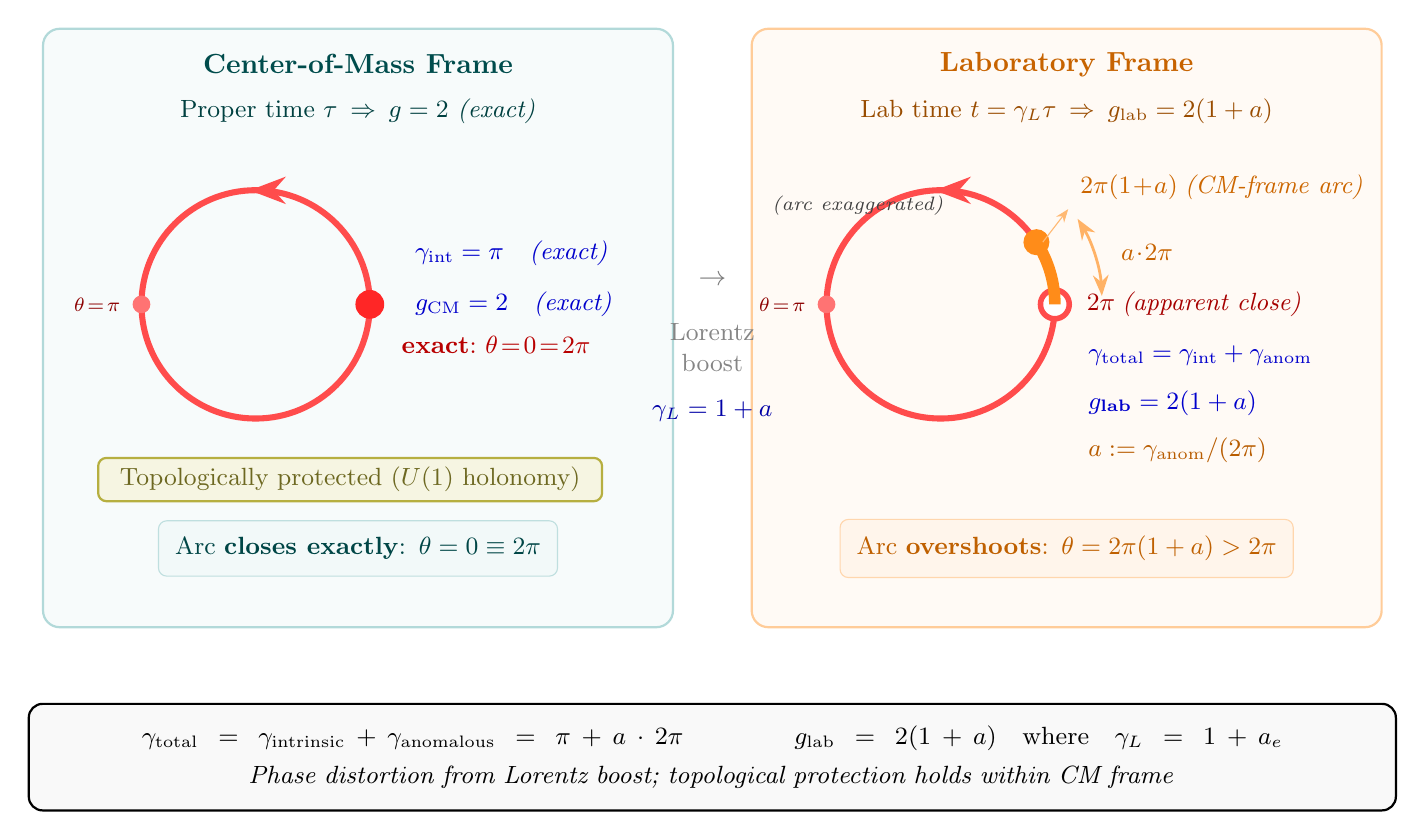
\begin{tikzpicture}[>=Stealth, font=\small]

%%====================================================
%% LEFT BOX — CENTER-OF-MASS FRAME
%% x in [-8.5, -0.5],  y in [-3.2, 4.4]
%%====================================================
\draw[thick, rounded corners=6pt, fill=teal!3, draw=teal!30]
  (-8.5, -3.2) rectangle (-0.5, 4.4);

%% Title + subtitle
\node[font=\normalsize\bfseries, teal!60!black] at (-4.5, 3.95)
  {Center-of-Mass Frame};
\node[font=\small, teal!50!black] at (-4.5, 3.35)
  {Proper time $\tau$\enspace $\Rightarrow$\enspace $g = 2$ \textit{(exact)}};

%% Circle: center (-5.8, 0.9), radius 1.45cm — full CCW red orbit
\draw[red!70, line width=2.2pt] (-4.35, 0.9) arc (0:360:1.45cm);
%% CCW arrow at top
\draw[red!70, ->, line width=2.2pt]
  ({-5.8+1.45*cos(87)}, {0.9+1.45*sin(87)}) --
  ({-5.8+1.45*cos(93)}, {0.9+1.45*sin(93)});
%% θ=π dot (leftmost)
\filldraw[red!55] (-7.25, 0.9) circle (3.0pt);
\node[left=4pt, font=\scriptsize, red!55!black] at (-7.25, 0.9) {$\theta\!=\!\pi$};
%% Exact closure: FILLED dot at θ=0=2π
\filldraw[red!85] (-4.35, 0.9) circle (5.0pt);
\node[anchor=north west, xshift=8pt, yshift=-8pt, font=\small, red!72!black] at (-4.35, 0.9)
  {\textbf{exact}:\ $\theta\!=\!0\!=\!2\pi$};

%% Annotations — right side of circle (x > -4.1)
\node[anchor=west, font=\small, blue!80!black] at (-3.9, 1.55)
  {$\gamma_{\text{int}} = \pi$\quad\textit{(exact)}};
\node[anchor=west, font=\small, blue!80!black] at (-3.9, 0.90)
  {$g_{\text{CM}} = 2$\quad\textit{(exact)}};

%% Topological protection badge — below circle (circle bottom at y≈0.9-1.45=-0.55)
\draw[olive!65, rounded corners=3pt, fill=olive!8, thick]
  (-7.8, -1.60) rectangle (-1.4, -1.05);
\node[font=\small, olive!70!black] at (-4.6, -1.32)
  {Topologically protected ($U(1)$ holonomy)};

%% Key result box
\node[draw=teal!25, rounded corners=3pt, fill=teal!5,
  font=\small, text=teal!55!black, inner sep=6pt] at (-4.5, -2.20)
  {Arc \textbf{closes exactly}:\enspace $\theta = 0 \equiv 2\pi$};

%%====================================================
%% RIGHT BOX — LABORATORY FRAME
%% x in [0.5, 8.5],  y in [-3.2, 4.4]
%%====================================================
\draw[thick, rounded corners=6pt, fill=orange!4, draw=orange!40]
  (0.5, -3.2) rectangle (8.5, 4.4);

%% Title + subtitle
\node[font=\normalsize\bfseries, orange!78!black] at (4.5, 3.95)
  {Laboratory Frame};
\node[font=\small, orange!60!black] at (4.5, 3.35)
  {Lab time $t = \gamma_L\tau$\enspace $\Rightarrow$\enspace $g_{\text{lab}} = 2(1+a)$};

%% Circle: center (2.9, 0.9), radius 1.45cm
\draw[red!70, line width=2.2pt] (4.35, 0.9) arc (0:360:1.45cm);
%% CCW arrow at top
\draw[red!70, ->, line width=2.2pt]
  ({2.9+1.45*cos(87)}, {0.9+1.45*sin(87)}) --
  ({2.9+1.45*cos(93)}, {0.9+1.45*sin(93)});
%% θ=π dot (leftmost)
\filldraw[red!55] (1.45, 0.9) circle (3.0pt);
\node[left=4pt, font=\scriptsize, red!55!black] at (1.45, 0.9) {$\theta\!=\!\pi$};
%% Open dot at θ=0 (apparent close, lab frame)
\filldraw[white] (4.35, 0.9) circle (5.2pt);
\draw[red!70, line width=2.0pt] (4.35, 0.9) circle (5.2pt);
\node[anchor=west, xshift=8pt, font=\small, red!65!black] at (4.35, 0.9)
  {$2\pi$\;\textit{(apparent close)}};
%% Orange arc: excess a·2π (exaggerated, 0→33°)
\draw[orange!90, line width=4.2pt] (4.35, 0.9) arc (0:33:1.45cm);
\filldraw[orange!90]
  ({2.9+1.45*cos(33)},{0.9+1.45*sin(33)}) circle (4.5pt);
%% Leader from orange dot to label
\node[anchor=south west, font=\small, orange!80!black]
  (cmLabel) at (4.55, {0.9+1.45*sin(33)+0.42})
  {$2\pi(1\!+\!a)$\;\textit{(CM-frame arc)}};
\draw[orange!55, thin, ->]
  ({2.9+1.45*cos(33)+0.08},{0.9+1.45*sin(33)}) -- (4.52, {0.9+1.45*sin(33)+0.42});
%% Double-arrow for gap
\draw[<->, orange!60, line width=1.0pt]
  ({2.9+2.05*cos(3)},{0.9+2.05*sin(3)}) arc (3:32:2.05cm);
\node[font=\small, orange!78!black]
  at ({2.9+2.70*cos(14)},{0.9+2.70*sin(14)}) {$a\!\cdot\!2\pi$};
\node[font=\scriptsize, gray!50!black] at (1.85, 2.15) {\textit{(arc exaggerated)}};

%% Berry phase decomposition — right area
\node[anchor=west, font=\small, blue!80!black] at (4.65, 0.25)
  {$\gamma_{\text{total}} = \gamma_{\text{int}} + \gamma_{\text{anom}}$};
\node[anchor=west, font=\small\bfseries, blue!80!black] at (4.65, -0.35)
  {$g_{\text{lab}} = 2(1+a)$};
\node[anchor=west, font=\small, orange!72!black] at (4.65, -0.95)
  {$a := \gamma_{\text{anom}}/(2\pi)$};

%% Key result box
\node[draw=orange!32, rounded corners=3pt, fill=orange!8,
  font=\small, text=orange!75!black, inner sep=6pt] at (4.5, -2.20)
  {Arc \textbf{overshoots}:\enspace $\theta = 2\pi(1+a) > 2\pi$};

%%====================================================
%% CENTRE — Lorentz boost arrow
%%====================================================
\node[font=\normalsize\bfseries, black!52] at (0, 1.20) {$\rightarrow$};
\node[font=\small, black!48, align=center] at (0, 0.35)
  {Lorentz\\boost};
\node[font=\small, blue!65!black, align=center] at (0, -0.45)
  {$\gamma_L = 1+a$};

%%====================================================
%% BOTTOM STRIP — unifying equation
%%====================================================
\node[draw, thick, rounded corners=5pt, fill=gray!5,
  text width=16.8cm, font=\small, align=center, inner sep=8pt]
  at (0, -4.85) {
  $\gamma_{\text{total}} = \gamma_{\text{intrinsic}} + \gamma_{\text{anomalous}} = \pi + a\cdot 2\pi$
  \qquad\qquad
  $g_{\text{lab}} = 2(1+a)$\quad where\quad $\gamma_L = 1 + a_e$\\[3pt]
  \textit{Phase distortion from Lorentz boost; topological protection holds within CM frame}
};

\end{tikzpicture}%
}

% ========================================
% TikZ macro #5 (fifth citation: fig:zpe_ladder)
% Usage: \figZpeLadder
%
% Design:
%   - Single parabolic potential V(x) ∝ (Te2 - Te1) centered on axis
%   - Four energy levels n=0,1,2,3 with Hermite-Gaussian wavefunctions
%   - Kernel A / Kernel B as orange dashed vertical boundaries
%   - Absorption arrow (yellow, n=0→1) and emission arrow (orange, n=2→1)
%   - Right-side annotations: geometric floor ½E₀ and level spacing ℏω
%   - Graph body shifted xshift=-1cm; annotations placed outside scope
% ========================================
\newcommand{\figZpeLadder}{%
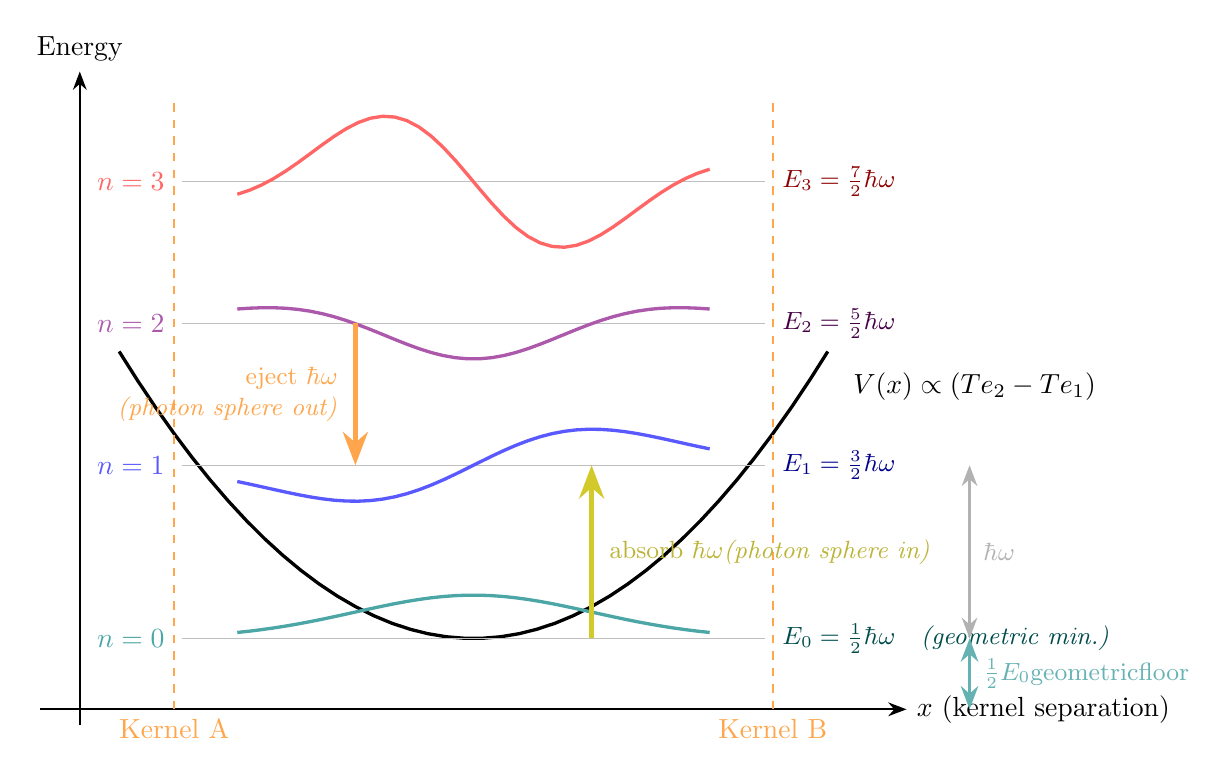
\begin{tikzpicture}[>=Stealth, font=\normalsize]

%% ── Graph elements shifted 1cm to the left ──────────────────
\begin{scope}[xshift=-1cm]

%% ── Axes ─────────────────────────────────────────────────────
\draw[thick, ->] (-5.5, -0.3) -- (5.5, -0.3)
  node[right] {$x$ (kernel separation)};
\draw[thick, ->] (-5.0, -0.5) -- (-5.0, 7.8)
  node[above] {Energy};

%% ── Potential curve (parabola) ───────────────────────────────
\draw[very thick, black]
  plot[domain=-4.5:4.5, samples=40] (\x, {0.18*\x*\x + 0.6});
\node[right, font=\normalsize] at (4.7, 3.8) {$V(x) \propto (Te_2 - Te_1)$};

%% ── Kernel positions ─────────────────────────────────────────
\draw[orange!70, dashed, thick] (-3.8, -0.3) -- (-3.8, 7.5);
\draw[orange!70, dashed, thick] ( 3.8, -0.3) -- ( 3.8, 7.5);
\node[orange!70, below, font=\normalsize] at (-3.8, -0.3) {Kernel A};
\node[orange!70, below, font=\normalsize] at ( 3.8, -0.3) {Kernel B};

%% ── Wavefunctions ────────────────────────────────────────────
%% Levels: n=0 @ y=0.6, n=1 @ y=2.8, n=2 @ y=4.6, n=3 @ y=6.4
%% Spacing = 1.8 units; distance from x-axis (-0.3) to n=0 = 0.9 = spacing/2

%% n=0  Gaussian (ground state)
\draw[gray!50] (-3.7, 0.6) -- (3.7, 0.6);
\draw[teal!70, very thick]
  plot[domain=-3.0:3.0, samples=40]
  (\x, {0.6 + 0.55*exp(-0.22*\x*\x)});
\node[left, teal!70] at (-3.8, 0.6) {$n=0$};
\node[right, font=\small, teal!60!black] at (3.8, 0.6)
  {$E_0 = \tfrac{1}{2}\hbar\omega$\quad\textit{(geometric min.)}};

%% n=1  Hermite H_1 ~ x·exp(-x²)
\draw[gray!50] (-3.7, 2.8) -- (3.7, 2.8);
\draw[blue!65, very thick]
  plot[domain=-3.0:3.0, samples=40]
  (\x, {2.8 + 0.50*\x*exp(-0.22*\x*\x)});
\node[left, blue!65] at (-3.8, 2.8) {$n=1$};
\node[right, font=\small, blue!55!black] at (3.8, 2.8)
  {$E_1 = \tfrac{3}{2}\hbar\omega$};

%% n=2  Hermite H_2 ~ (2x²-1)·exp(-x²)
\draw[gray!50] (-3.7, 4.6) -- (3.7, 4.6);
\draw[violet!65, very thick]
  plot[domain=-3.0:3.0, samples=40]
  (\x, {4.6 + 0.45*(2*0.22*\x*\x - 1)*exp(-0.22*\x*\x)});
\node[left, violet!65] at (-3.8, 4.6) {$n=2$};
\node[right, font=\small, violet!55!black] at (3.8, 4.6)
  {$E_2 = \tfrac{5}{2}\hbar\omega$};

%% n=3  Hermite H_3 ~ x·(2x²-3)·exp(-x²)
\draw[gray!50] (-3.7, 6.4) -- (3.7, 6.4);
\draw[red!60, very thick]
  plot[domain=-3.0:3.0, samples=40]
  (\x, {6.4 + 0.40*\x*(2*0.22*\x*\x - 3)*exp(-0.22*\x*\x)});
\node[left, red!60] at (-3.8, 6.4) {$n=3$};
\node[right, font=\small, red!55!black] at (3.8, 6.4)
  {$E_3 = \tfrac{7}{2}\hbar\omega$};

%% ── Transition arrows ────────────────────────────────────────

%% Absorption (n=0 → n=1): yellow upward arrow
\draw[->, yellow!80!black, very thick, line width=2.0pt]
  (1.5, 0.6) -- (1.5, 2.8);
\node[right, yellow!70!black, font=\small] at (1.6, 1.7)
  {absorb $\hbar\omega$\\\textit{(photon sphere in)}};

%% Emission (n=2 → n=1): orange downward arrow
\draw[->, orange!70, very thick, line width=2.0pt]
  (-1.5, 4.6) -- (-1.5, 2.8);
\node[left, orange!70, font=\small, align=right] at (-1.6, 3.7)
  {eject $\hbar\omega$\\\textit{(photon sphere out)}};

\end{scope}  %% xshift=-1cm end

%% ── Annotations (outside xshift scope) ──────────────────────

%% Zero-point energy floor: x-axis (-0.3) to n=0 level (0.6)
\draw[<->, teal!60, line width=1.2pt] (5.3, -0.30) -- (5.3, 0.6);
\node[right, teal!60, font=\small] at (5.35, 0.15)
  {$\tfrac{1}{2}E_0$\\geometric\\floor};

%% Level spacing: n=0 to n=1
\draw[<->, gray!60, line width=1.0pt] (5.3, 0.6) -- (5.3, 2.8);
\node[right, gray!60, font=\small] at (5.35, 1.7) {$\hbar\omega$};

\end{tikzpicture}%
}


\begin{document}

\title{Geometric Origin of $g = 2$ in the 0-Sphere Model:\\ U(1) Fiber Bundle and Dual-Frame Phase Decomposition}

\author{Satoshi Hanamura} \email{hana.tensor@gmail.com}
\date{March 28, 2026}
%\date{\today}

\begin{abstract}
We establish the geometric phase structure of the 0-Sphere electron model, demonstrating that its internal 2$\pi$ periodicity naturally accommodates two independent degrees of freedom: the center-of-mass frame and the laboratory observation frame. Beginning from energy conservation constraints, we prove that the kinetic energy term mandates 2$\pi$ periodicity through the single-valuedness requirement of the state function. This periodicity induces a principal $\Uone$ fiber bundle structure, wherein the Berry phase $\gamma_{\text{intrinsic}} = \pi$ emerges as a coordinate-invariant quantity, geometrically necessitating $g = 2$ in the proper-time frame. In the laboratory frame, Lorentz projection introduces a phase distortion $\gamma_{\text{anomalous}}$, yielding the decomposition $\gamma_{\text{total}} = \gamma_{\text{intrinsic}} + \gamma_{\text{anomalous}}$ and the corresponding $g$-factor structure $g_{\text{lab}} = 2(1 + a)$ where $a := \gamma_{\text{anomalous}}/(2\pi)$. A central result of this analysis is an arc-length argument identifying the geometric mechanism of $a_e$: rotational Lorentz contraction shortens the internal orbital arc $2\pi r \in [L]$ by the factor $1/(1+a_e)$, the same mechanism by which a muon's path length $L_0 \in [L]$ is extended to $\gamma_L L_0$ during atmospheric transit. This inverse calculation~\cite{Hanamura_2026_35} yields $v_{\text{ZB}} \approx 0.04c$ and identifies $\gamma_L = 1+a_e$ as a structural consequence of special relativity applied to the internal orbital motion. The anomalous magnetic moment and the muon lifetime experiment are thereby identified as two manifestations of the same relativistic length-extension structure. Furthermore, we identify a hierarchical phase structure within the single $2\pi$ cycle: three coexisting periodicities ($\pi$, $2\pi$, $4\pi$) correspond, via the spin-periodicity relation $s = 2\pi/T$, to spin-2, spin-1, and spin-1/2 respectively, suggesting a structural correspondence with gravitational, electromagnetic, and weak gauge symmetries. This framework provides a geometric foundation that may offer structural insight into both the $g$-factor structure and the origin of gauge symmetries. We emphasize that this work establishes the theoretical architecture; the physical validation of the gauge symmetry correspondence and the precise quantitative derivation of $v_{\text{ZB}}$ remain subjects for future investigation.
\end{abstract}

\maketitle

\section{Introduction}
\label{sec:introduction}

The Berry phase, first identified by Michael Berry in 1984~\cite{Berry1984}, represents a geometric phase acquired by a quantum system traversing a closed path in parameter space. This phase is gauge-invariant modulo $2\pi$ and arises from the curvature of the parameter manifold, not from dynamical forces. The 0-Sphere Model~\cite{Hanamura_2018_01,Hanamura_2025_24} proposes an internal structure for the electron in which two energy kernels $A$ and $B$ exchange thermal potential energy via an oscillating photon sphere; this internal degree of freedom, characterized by Zitterbewegung motion~\cite{Schrodinger1930,Dirac1928}, generates emergent quantum phenomena including spin~\cite{Hanamura_2025_26} and, as demonstrated here, the $g$-factor structure.

The present paper establishes that the internal $2\pi$ periodicity of this oscillation induces a principal $\Uone$ fiber bundle, whose Berry holonomy $\gamma_{\text{intrinsic}} = \pi$ geometrically necessitates $g_{\text{CM}} = 2$ in the proper-time frame without any perturbative input. In the laboratory frame, a Lorentz boost introduces a phase distortion $\gamma_{\text{anomalous}}$, yielding $g_{\text{lab}} = 2(1+a)$ where $a := \gamma_{\text{anomalous}}/(2\pi)$. An arc-length argument further identifies $\gamma_L = 1 + a_e$ as a direct consequence of rotational Lorentz contraction applied to the internal orbital motion---a structure algebraically identical to the muon lifetime extension---providing a geometric bridge between two phenomena conventionally treated by separate theoretical frameworks.

A note on interpretation: the 0-Sphere Model does not identify the internal states $|A\rangle$ and $|B\rangle$ with simultaneous superposition but treats them as physically distinct, time-ordered phases of the internal oscillation. This realist reading is developed in Section~\ref{sec:realist_interpretation} and contrasted with the standard superposition picture.

\subsection*{Synopsis}

The paper is organized as follows. Section~\ref{sec:motivation} develops the conceptual motivation for the $\Uone$ fiber bundle geometry and states the principal claims precisely. Section~\ref{sec:0sphere} defines the 0-Sphere internal structure and the energy parameterization. Section~\ref{sec:hamiltonian} proves the $2\pi$ periodicity of the quantum state from the single-valuedness requirement. Section~\ref{sec:u1fiber} constructs the principal $\Uone$ bundle, derives the Berry connection and holonomy, and establishes gauge invariance and topological protection. Section~\ref{sec:dual_frame} analyzes the dual-frame structure, deriving the phase decomposition $\gamma_{\text{total}} = \pi + a \cdot 2\pi$ and the laboratory $g$-factor $g_{\text{lab}} = 2(1+a)$ via Thomas precession and the arc-length argument. Section~\ref{sec:discussion} collects the Discussion, including the geometric interpretation of the zero-point energy (Section~\ref{sec:zpe_reinterpretation}), the realist reading of the Bloch sphere (Section~\ref{sec:realist_interpretation}), the algebraic selection of the thermodynamic spin classification (Section~\ref{sec:classification_argument}), and the hierarchical phase--gauge symmetry correspondence (Section~\ref{sec:gauge_correspondence}).

% ─────────────────────────────────────────────────────────────────────────────
\section{Motivation and Conceptual Overview}
\label{sec:motivation}
% ─────────────────────────────────────────────────────────────────────────────

\subsection{Emergence of the \texorpdfstring{$\Uone$}{U(1)} Fiber Bundle from Internal Periodicity}
\label{sec:why_u1}

The $\Uone$ principal fiber bundle that organizes this paper is not postulated as a gauge principle but derived from the internal dynamics of the 0-Sphere Model through a three-step logical chain.

\subsubsection{Step 1: The $2\pi$ Period Is Uniquely Determined}

The kinetic energy of the oscillating photon sphere takes the form $T(\theta) = \frac{E_0}{2}\sin^2\theta$. As a scalar, this function has period $\pi$. However, the single-valuedness requirement on the quantum state $|\psi(\theta)\rangle$ is more restrictive: it rules out $\pi$ (too short for a spinor) and $4\pi$ (the full spinor period) as the fundamental period of the complete state, selecting $2\pi$ as the unique minimum period compatible with spin-$\tfrac{1}{2}$ geometry. This is established as Lemma~\ref{lem:single_valued} in Section~\ref{sec:hamiltonian}.

\subsubsection{Step 2: The $2\pi$ Period Defines a Circle, and a Circle Defines a Bundle}

Once the internal parameter $\theta$ is identified as a $2\pi$-periodic variable, it parametrizes a circle $\Sone \simeq \mathbb{R}/(2\pi\mathbb{Z})$. This circle is the base space of a fiber bundle. The residual degree of freedom at each point $\theta$---the complex phase $e^{i\phi}$---constitutes the fiber. Together, base $\Sone$ and fiber $\Uone = \{e^{i\phi} \mid \phi \in \mathbb{R}\}$ assemble into the principal $\Uone$ bundle $P = \Sone \times \Uone$ with projection $\pi : (\theta, e^{i\phi}) \mapsto \theta$. No external gauge principle is invoked; the bundle is a geometric consequence of the dynamical period.

\subsubsection{Step 3: The Bundle Carries a Non-Trivial Holonomy}

A principal $\Uone$ bundle over $\Sone$ admits a connection 1-form, the Berry connection $A_\theta(\theta) := \langle \psi(\theta) | i\partial_\theta | \psi(\theta) \rangle$. For the internal state of the 0-Sphere Model, this evaluates to $A_\theta = \frac{1}{2}\cos\theta$ (Section~\ref{sec:u1fiber}). The holonomy around the closed base circle receives a boundary contribution from the non-single-valued gauge representative, yielding $\gamma_{\text{intrinsic}} = \pi$. This value is topologically protected: it equals half the solid angle $\Omega = 2\pi$ subtended by the equatorial trajectory on the Bloch sphere, and it is invariant under continuous deformations of the path.

\subsection{Principal Claims}
\label{sec:claims}

\subsubsection{\texorpdfstring{$g = 2$}{g = 2} as a Geometric Theorem}

The identification $g := 2\gamma/\pi$---where $\gamma$ is the Berry holonomy accumulated per internal cycle---together with the computed value $\gamma_{\text{intrinsic}} = \pi$ yields $g_{\text{CM}} = 2$ as a theorem (Theorem~\ref{thm:g_equals_2}). The value 2 is not substituted; it is the unique output of a geometric definition applied to a topologically protected invariant. Any perturbative correction to $g_{\text{CM}}$ in the proper-time frame would require a discontinuous change in the holonomy, which is forbidden by the $\mathbb{Z}_2$ topological protection of the $\mathrm{SU}(2)$ double cover structure.

\subsubsection{Dual-Frame Decomposition of the \texorpdfstring{$g$}{g}-Factor}

A laboratory observer is related to the proper-time frame by a Lorentz boost whose velocity is set by the Zitterbewegung speed $v_{\text{ZB}}$. This boost distorts the internal phase cycle, generating an anomalous Berry phase $\gamma_{\text{anomalous}}$. The total holonomy decomposes as
\begin{equation}
\gamma_{\text{total}} = \underbrace{\pi}_{\text{intrinsic}} + \underbrace{a \cdot 2\pi}_{\text{anomalous}},
\label{eq:gamma_decomp_intro}
\end{equation}
yielding $g_{\text{lab}} = 2(1+a)$. The Foucault pendulum provides the classical prototype: the equatorial observer measures zero precession ($g_{\text{CM}} = 2$), while an observer at geographic latitude $\varphi > 0$ observes a precession $2\pi\sin\varphi$, corresponding to $\gamma_{\text{anomalous}}$.

\subsubsection{The Arc-Length Argument and the Muon Analogy}

Rotational Lorentz contraction shortens the internal orbital arc $2\pi r$ by the factor $1/(1+a_e)$, from which the Zitterbewegung velocity $v_{\text{ZB}} \approx 0.04c$ is recovered~\cite{Hanamura_2026_35}. The resulting Lorentz factor $\gamma_L = 1/\sqrt{1-v_{\text{ZB}}^2/c^2} \approx 1 + a_e$ generates the excess arc $(\gamma_L - 1)\cdot 2\pi r = a_e \cdot 2\pi r$, which is the geometric source of $\gamma_{\text{anomalous}}$. This structure is algebraically identical to the muon lifetime extension: a muon at $v \approx c$ traverses the atmosphere because its laboratory path length $\gamma_L L_0$ is extended by the same Lorentz factor. The forward derivation---from Thomas precession to $v_{\text{ZB}}$ independently of $a_e$---remains the central open task of the programme.

\subsubsection{Hierarchical Phase Structure and Gauge Symmetry}

A single $2\pi$ internal cycle hosts three coexisting periodicities: the half-angle thermal energy ($\pi$-periodic), the kinetic energy ($2\pi$-periodic), and the Thomas angular velocity ($4\pi$-periodic). Applying the spin-periodicity relation $s = 2\pi/T$ maps these to spin-2, spin-1, and spin-$\tfrac{1}{2}$ respectively. This numerical correspondence with the gauge bosons of gravity, electromagnetism, and the weak interaction is developed in Section~\ref{sec:gauge_correspondence} as a phenomenological correspondence, explicitly distinguished from the rigorous results of the preceding sections.

\section{Definition of the 0-Sphere Internal Structure}
\label{sec:0sphere}

\subsection{Discrete Two-Point Structure}

The 0-Sphere topology $\Sphere = \{A, B\}$ consists of two discrete points representing energy kernels within the electron. Following the foundational framework of Ref.~\cite{Hanamura_2018_01}, the electron contains two bare spinors exchanging thermal potential energy via an oscillating photon sphere. Energy is distributed among three components:
\begin{equation}
E_0 = Te_1(t) + Te_2(t) + E_{\text{transition}}(t),
\label{eq:energy_distribution}
\end{equation}
where $Te_1$ and $Te_2$ denote the thermal potential energies of spinors 1 and 2 localized at kernels $A$ and $B$, respectively, and $E_{\text{transition}}$ represents the transitional kinetic energy associated with the photon sphere oscillating between them~\cite{Hanamura_2018_01}.



\subsection{Emergent Angular Variable}

The periodic exchange of energy between kernels $A$ and $B$ induces a natural parameterization via an angular variable $\theta$. We define the internal phase parameter:
\begin{equation}
\theta := \omega \tau,
\label{eq:theta_definition}
\end{equation}
where $\tau$ denotes proper time in the center-of-mass frame and $\omega$ is the internal oscillation angular frequency.

The energy components admit the explicit parameterization~\cite{Hanamura_2018_01}:
\begin{align}
Te_1(\theta) &:= E_A(\theta) = E_0 \cos^4(\theta/2), \label{eq:EA} \\
Te_2(\theta) &:= E_B(\theta) = E_0 \sin^4(\theta/2), \label{eq:EB} \\
E_{\text{transition}}(\theta) &= \frac{E_0}{2} \sin^2(\theta). \label{eq:Etrans}
\end{align}
The fourth-power structure of $Te_1$ and $Te_2$ arises from the Stefan-Boltzmann radiation law governing the perfect black-body spinors~\cite{Hanamura_2018_01}. One may verify by direct calculation that Eq.~\eqref{eq:energy_distribution} is satisfied identically for all $\theta$ using the trigonometric identity $\cos^4(x) + \sin^4(x) = 1 - \frac{1}{2}\sin^2(2x)$ (see Appendix~\ref{app:energy_conservation}). The temporal evolution of these three components---confirming $\pi$ periodicity of scalar energy quantities alongside the $2\pi$ periodicity required by the complete quantum state---is visualized in Ref.~\cite{Hanamura_2026_35}, Fig.~1.

The periodic nature of this exchange necessitates an identification:
\begin{equation}
\theta \sim \theta + 2\pi,
\label{eq:periodicity}
\end{equation}
establishing $\theta$ as an angular coordinate. The geometric necessity of the period $2\pi$ (rather than $\pi$ or $4\pi$) is demonstrated rigorously in Section~\ref{sec:hamiltonian}.



\section{Hamiltonian Structure and 2$\pi$ Periodicity}
\label{sec:hamiltonian}

\subsection{Kinetic Energy and Periodicity}

From Eq.~\eqref{eq:Etrans}, the transitional kinetic energy component is:
\begin{equation}
T(\theta) = \frac{E_0}{2} \sin^2(\theta).
\label{eq:kinetic}
\end{equation}

Employing the trigonometric identity $\sin^2(\theta) = (1 - \cos(2\theta))/2$, we obtain:
\begin{equation}
T(\theta) = \frac{E_0}{4}(1 - \cos(2\theta)).
\label{eq:kinetic_explicit}
\end{equation}

Evidently, $T(\theta + \pi) = T(\theta)$, suggesting a periodicity of $\pi$ for the energy (a scalar quantity). However, the physical entity under consideration is not merely the energy but the complete quantum state, which is a vector quantity in Hilbert space.

Three distinct phase structures coexist within a single internal cycle $\theta: 0 \to 2\pi$ (kernel transition $A \to B \to A'$).

\textbf{(1) Half-angle structure} ($\theta/2$): The thermal potential energy $Te_1 = E_0\cos^4(\theta/2)$ undergoes only a $\pi$ phase change over the full $2\pi$ interval, with a single maximum at $\theta = 0$ (spinor 1 at kernel $A$) and minimum at $\theta = \pi$ (spinor 2 at kernel $B$). This $\pi$ periodicity is a property of the scalar thermal potential energy, not of the quantum state. The fourth-power dependence traces directly to the Stefan-Boltzmann radiation law~\cite{Hanamura_2018_01}, and the normalized maximum reaches unity: $Te_1^{\max}/E_0 = 1$.

The designation ``potential energy'' for $Te_1$ and $Te_2$ is physically justified through their role as a \emph{radiation gradient}. Computing the difference and differentiating with respect to $\theta$:
\begin{equation}
\frac{d}{d\theta}(Te_2 - Te_1)
= \frac{d}{d\theta}\,E_0\!\left[\sin^4(\theta/2) - \cos^4(\theta/2)\right]
= E_0\sin\theta,
\label{eq:radiation_gradient}
\end{equation}
which serves as the driving force for the photon sphere~\cite{Hanamura_2018_01}. The pair $(Te_1, Te_2)$ thus constitutes a gradient-generating source: the photon sphere is displaced toward the region of lower thermal potential, executing simple harmonic motion exactly as a particle in a conservative potential well. This gradient structure is precisely why $Te_1$ and $Te_2$ merit the name \emph{thermal potential energies} rather than mere oscillating scalar quantities.

The physical justification for this conservative-potential analogy admits a deeper geometric grounding through the radiative nature of the energy exchange. Since $Te_1$ and $Te_2$ represent thermal radiation fields, the photon sphere---as a radiative entity mediating energy between them---is governed by Snell's law of refraction across the internal thermal medium. In a continuously varying medium, Snell's law is equivalent to Fermat's principle of least optical path, which in turn identifies the physical trajectory as the unique geodesic of the internal geometry. This chain of equivalences,
\begin{align}
&\text{radiative transport}
\;\Rightarrow\; \text{Snell's law} \nonumber\\
&\;\Rightarrow\; \text{Fermat's principle}
\;\Rightarrow\; \text{geodesic uniqueness},
\label{eq:snell_geodesic}
\end{align}
provides the geometric mechanism underlying the thermal geodesic framework of Ref.~\cite{Hanamura_2025_24}. The scalar potential $\phi := Te_2 - Te_1$ thereby acquires a well-defined status as a conservative scalar potential: the photon sphere path is \emph{uniquely determined} by the internal geometry, fixing the value of $\int \nabla\phi \cdot d\boldsymbol{\ell}$ along the physically realized geodesic path. Energy conservation (Eq.~\ref{eq:energy_distribution}) is thus not an imposed axiom but a geometric consequence of the radiative geodesic structure. This equivalence chain also supplies the physical content of the axiom ``free particles follow geodesics'': in the 0-Sphere model that axiom is not postulated but derived from the radiative character of the photon sphere via Snell's law.

\textbf{(2) Normal-angle structure} ($\theta$): The radiation gradient (Eq.~\ref{eq:radiation_gradient}) acts as the driving force, producing the kinetic energy of the photon sphere:
\begin{equation}
T(\theta) = \frac{E_0}{2}\sin^2(\theta),
\end{equation}
with energy peaks at $\theta = \pi/2$ and $3\pi/2$ within the $2\pi$ interval. The $2\pi$ periodicity of this component establishes the minimal period of the complete quantum state, as demonstrated in Lemma~\ref{lem:single_valued}.

This structure bears a formal resemblance to classical simple harmonic motion: the photon sphere oscillates back and forth between kernels $A$ and $B$, driven by the thermal potential gradient, in direct analogy with a mass on a spring. However, a fundamental distinction from classical harmonic oscillation must be noted. In classical mechanics, there exists a phase point at which all potential energy is converted entirely into kinetic energy, yielding a normalized kinetic maximum of unity. In the 0-Sphere Model, the normalized kinetic energy maximum is $T^{\max}/E_0 = 1/2$, never reaching the total energy $E_0$. This ceiling arises from the Stefan-Boltzmann fourth-power structure of $Te_1$ and $Te_2$: the thermal potential energy distributed across both spinors cannot be fully transferred to the photon sphere at any single phase point. The factor $\frac{1}{2}$ is therefore not a free parameter but a thermodynamic consequence of the black-body radiation law governing the internal spinors.

\textbf{(3) Double-angle structure} ($2\theta$): The Thomas angular velocity $\Omega_T \propto \frac{1}{2}\sin(2\theta)$ exhibits a double-angle phase structure within the $2\pi$ interval, with normalized maximum $|\Omega_T|^{\max} = 1/2$. Although $\Omega_T$ completes two sign reversals within $[0, 2\pi]$, a full spinorial return requires a $4\pi$ cycle, consistent with the $-1$ phase factor under $2\pi$ rotation (Eq.~\ref{eq:spinor_periodicity}).

The physical origin of this $4\pi$ periodicity is identified as follows. During a single one-way transit of the photon sphere from kernel $A$ to kernel $B$ (spanning $\theta: 0 \to \pi$), the Thomas angular velocity completes one full oscillation cycle ($0 \to +\tfrac{1}{2} \to 0$), corresponding to one complete revolution of angular momentum. The return transit ($\theta: \pi \to 2\pi$) generates an identical angular momentum profile ($0 \to +\tfrac{1}{2} \to 0$). Because both half-cycles produce the same waveform, they are indistinguishable from the amplitude alone. This double traversal within $[0, 2\pi]$ is the geometric source of the electron's $720°$ spinor periodicity: only after the photon sphere completes two full round trips ($\theta: 0 \to 4\pi$) does the spinorial state return to its original value with $+1$ phase.

The two half-cycles are distinguished by the thermodynamic state of kernel $A$. In the interval $\theta \in [0, \pi]$, kernel $A$ is in the radiation phase ($\partial Te_1/\partial t < 0$, energy decreasing), corresponding to the negative-energy solution in the Dirac reinterpretation~\cite{Hanamura_2018_01}; we identify this half-cycle as the \textbf{spin-up state}. In the interval $\theta \in [\pi, 2\pi]$, kernel $A$ is in the absorption phase ($\partial Te_1/\partial t > 0$, energy increasing), corresponding to the positive-energy solution; we identify this as the \textbf{spin-down state}. This identification is our own interpretation, and is depicted in the spin-up and spin-down annotations of Fig.~\ref{fig:three_phases} below.

A second classification scheme is possible, based directly on the sign of $\Omega_T$. Since $\Omega_T = \tfrac{1}{2}\sin(2\theta)$ reverses sign at $\theta = \pi/2$, one may assign spin-up to the phases $\Omega_T > 0$ (i.e., $\theta \in (0, \pi/2) \cup (\pi, 3\pi/2)$) and spin-down to $\Omega_T < 0$ (i.e., $\theta \in (\pi/2, \pi) \cup (3\pi/2, 2\pi)$). We call this the \textbf{kinematic classification}. Under this scheme, a complete spin-up/spin-down cycle is contained within a \emph{single half-period} $[0, \pi]$, and the photon sphere completes two such spin cycles within $[0, 2\pi]$.

This leads to a natural observation about scalability. The photon sphere oscillation has period $2\pi$; the Thomas angular velocity $\Omega_T \propto \sin(2\theta)$ oscillates at twice this frequency, with period $\pi$. The ratio of spinor periodicity to photon-sphere periodicity is therefore:
\begin{equation}
\frac{4\pi \text{ (spinor return)}}{2\pi \text{ (photon sphere return)}} = 2,
\label{eq:scalability_ratio}
\end{equation}
a consequence of the 2:1 frequency ratio between $\Omega_T$ and the photon-sphere oscillation. This provides an explicit mechanism by which the $720°$ spinor periodicity and the $360°$ photon-sphere periodicity coexist within a single dynamical system at different scales: they are related by the same factor of 2 that distinguishes SU(2) from SO(3).

The two classification schemes are compared in Fig.~\ref{fig:two_spin_schemes}. They are not mutually exclusive as physical descriptions; rather, they reflect two different questions one may ask of the same geometry:

The two schemes are compared in detail in Table~\ref{tab:spin_classification} and visualized in Fig.~\ref{fig:two_spin_schemes}.

\begin{enumerate}
\item \textbf{Thermodynamic classification} (adopted in this paper):
  \emph{In which thermodynamic phase is kernel $A$?}
  This assigns spin state by hemisphere on the Bloch sphere,
  preserving the geometric identification of the northern hemisphere
  ($\theta \in [0, \pi)$) with a single physical domain.
  It connects directly to the Dirac reinterpretation~\cite{Hanamura_2018_01}.

\item \textbf{Kinematic classification} (open alternative):
  \emph{What is the sign of the Thomas angular velocity?}
  This assigns spin state by the instantaneous direction of $\Omega_T$,
  placing a complete up/down cycle within each kernel transit $A \to B$.
  It explains the 2:1 scalability between spinor and photon-sphere periodicities
  more transparently.
\end{enumerate}

Resolving which classification is physically primary---or whether both describe complementary aspects of the same internal geometry---is left as an open question for future investigation. The thermodynamic classification is retained throughout the main body of this paper, with the kinematic alternative documented here as a direction for further theoretical development.


\begin{table*}[t!]
\centering
\caption{Comparison of Thermodynamic and Kinematic Spin-State Classification Schemes}
\label{tab:spin_classification}
\renewcommand{\arraystretch}{1.4}
\begin{tabular}{p{5.0cm}p{5.5cm}p{5.5cm}}
\toprule
\textbf{Criterion} & \textbf{Thermodynamic classification} & \textbf{Kinematic classification} \\
\midrule
Basis of assignment
  & Thermodynamic phase of kernel $A$
  & Sign of $\Omega_T = \tfrac{1}{2}\sin(2\theta)$ \\
\addlinespace[0.25cm]
Spin-up interval
  & $\theta \in [0, \pi)$
  & $\theta \in (0,\tfrac{\pi}{2}) \cup (\pi, \tfrac{3\pi}{2})$ \\
\addlinespace[0.25cm]
Spin-down interval
  & $\theta \in (\pi, 2\pi]$
  & $\theta \in (\tfrac{\pi}{2}, \pi) \cup (\tfrac{3\pi}{2}, 2\pi)$ \\
\addlinespace[0.25cm]
Span of one up/down cycle
  & $2\pi$ (full period)
  & $\pi$ (half period) \\
\addlinespace[0.25cm]
Bloch sphere correspondence
  & Northern/southern hemisphere (natural)
  & Equator as reversal point (reinterpretation required) \\
\addlinespace[0.25cm]
Connection to Dirac equation
  & Positive/negative energy solutions
  & No direct correspondence \\
\addlinespace[0.25cm]
Explanation of $720°$ periodicity
  & Amplitude indistinguishability of two half-cycles
  & 2:1 frequency ratio ($\Omega_T$ vs.\ photon sphere) \\
\addlinespace[0.25cm]
Origin of SU(2)/SO(3) factor of 2
  & Externally imposed
  & Emerges internally as $4\pi/2\pi = 2$ \\
\addlinespace[0.25cm]
Status in this paper
  & Adopted (primary classification)
  & Open alternative \\
\addlinespace[0.25cm]
Future direction
  & ---
  & Geometric origin of spin discreteness \\
\bottomrule
\end{tabular}
\vspace{0.2cm}
\begin{flushleft}
\footnotesize
\textbf{Note:} Comparison of two spin-state classification schemes arising from the internal dynamics of the 0-Sphere Model. The thermodynamic classification (left) is adopted throughout this paper and connects naturally to the Dirac reinterpretation and Bloch sphere geometry. The kinematic classification (right) offers a complementary perspective in which the SU(2)/SO(3) factor of 2 emerges transparently from the 2:1 frequency ratio between the Thomas angular velocity and the photon-sphere oscillation. Resolving which classification is physically primary is left as an open question; see Fig.~\ref{fig:two_spin_schemes} for visual comparison.
\end{flushleft}
\end{table*}

\begin{remark}[Continuity at the Spin-State Boundary]
\label{rem:continuity}
A potential concern arises from the representation of $\Omega_T$ in
Fig.~\ref{fig:three_phases}: the curve appears to exhibit a kink at $\theta = \pi$,
where the sign of $\Omega_T$ reflects upon the return transit $B \to A$.
We clarify that this is not a physical discontinuity.

At the turning points $\theta \in \{0, \pi, 2\pi\}$, the photon sphere momentarily
comes to rest: $v = 0$, and therefore
\begin{equation}
\Omega_T\big|_{\theta = \pi} \;\propto\; \bm{a} \times \bm{v}\big|_{\theta=\pi}
= \bm{a}(\pi) \times \mathbf{0} = \mathbf{0}.
\label{eq:omega_zero}
\end{equation}
Both the forward and return trajectories approach zero smoothly as $\theta \to \pi$,
so the curve is continuous ($C^0$) at this point.
Moreover, since the photon-sphere velocity varies as $v(\theta) \propto -\sin\theta$
near $\theta = \pi$, the derivative of $\Omega_T$ is also well-defined and finite there,
ensuring $C^1$ differentiability.
The apparent kink in Fig.~\ref{fig:three_phases} is therefore an artefact of plotting
two piecewise analytic expressions and does not reflect any physical discontinuity.

This observation has a deeper geometric significance.
The transition from spin-up ($\theta \in [0, \pi)$) to spin-down ($\theta \in (\pi, 2\pi]$)
on the Bloch sphere corresponds to passage from the northern hemisphere to the southern
hemisphere, i.e.\ from the ``front surface'' to the ``back surface'' of the sphere.
Classically, traversing the equator of a sphere reverses the outward normal, which might
suggest a discontinuity in the spin-state description.
The 0-Sphere Model circumvents this through a physical mechanism: at $\theta = \pi$,
the photon sphere halts ($v = 0$, $\Omega_T = 0$), providing a dynamical
\emph{rest point} at the equatorial boundary.
This rest point acts as a smooth ``handover'' between the two spin-state domains,
ensuring that the front-to-back transition on the Bloch sphere is accomplished
in a differentiably continuous manner.

We further note that this structure is structurally analogous to how the Dirac equation
resolves the sign ambiguity of $\sqrt{E^2 - m^2c^4}$: rather than accepting a branch cut
on the real axis, Dirac elevated the problem to a matrix (SU(2)) space in which
positive- and negative-energy solutions are connected smoothly via off-diagonal terms.
In the present model, $\Omega_T$ undergoes an analogous sign change at $\theta = \pi$,
and the SU(2) spinor space provides the covering structure within which this change is
analytically continuous.
Whether this analogy is coincidental or reflects a deeper common origin is a question
we leave for future investigation (see Appendix~\ref{app:su2_continuity} for a
detailed discussion).
\end{remark}


The coexistence of these three periodicities within a single fundamental cycle is the geometric foundation of the following lemma. The structural significance of the common $\frac{1}{2}$ amplitude shared by structures (2) and (3), and its visualization, are treated in Section~\ref{sec:half_factor}.

\begin{lemma}[State Function Single-Valuedness]
\label{lem:single_valued}
The physical state function $|\psi(\theta)\rangle$ must satisfy single-valuedness under the identification $\theta \sim \theta + T$ for some minimal period $T$. For spin-1/2 fermions, this imposes $T = 2\pi$.
\end{lemma}

\begin{proof}
The internal state admits a representation on the Bloch sphere as:
\begin{equation}
|\psi(\theta)\rangle = \cos(\theta/2)|A\rangle + \sin(\theta/2)|B\rangle,
\label{eq:state_real}
\end{equation}
where $|A\rangle$ and $|B\rangle$ denote the kernel states corresponding to the north and south poles, respectively.

Under $\theta \to \theta + 2\pi$:
\begin{align}
|\psi(\theta + 2\pi)\rangle &= \cos(\theta/2 + \pi)|A\rangle + \sin(\theta/2 + \pi)|B\rangle \nonumber \\
&= -\cos(\theta/2)|A\rangle - \sin(\theta/2)|B\rangle \nonumber \\
&= -|\psi(\theta)\rangle.
\label{eq:spinor_periodicity}
\end{align}

This sign change is the defining property of spinors under $2\pi$ rotation. Physically, $|\psi(\theta)\rangle$ and $-|\psi(\theta)\rangle$ represent identical quantum states, as the global phase is unobservable. However, a period of $\pi$ would yield:
\begin{equation}
|\psi(\theta + \pi)\rangle = -\cos(\theta/2)|A\rangle + \sin(\theta/2)|B\rangle,
\label{eq:pi_shift}
\end{equation}
which is orthogonal to $|\psi(\theta)\rangle$ and thus physically distinct. Therefore, the minimal period ensuring single-valuedness is $T = 2\pi$.
\end{proof}

\begin{remark}
While the scalar energy $T(\theta)$ exhibits $\pi$ periodicity, the vector state $|\psi(\theta)\rangle$ requires $2\pi$ periodicity for consistency. This distinction between scalar and spinorial periodicity is fundamental to the geometry of spin-1/2 systems.
\end{remark}

\subsection{Bloch Sphere Geometry and Berry Phase}
\label{sec:Berry_phase}

\textit{Classification assumption.} The analysis in this section and the remainder of the paper adopts the \emph{thermodynamic spin-state classification} (Fig.~\ref{fig:two_spin_schemes}(a)), in which spin-up corresponds to $\theta \in [0,\pi)$ (kernel $A$ in the radiation phase) and spin-down to $\theta \in (\pi, 2\pi]$ (absorption phase), with the hemisphere boundary at the transition point $\theta = \pi$. The alternative \emph{kinematic classification} (panel (b)), in which $\mathrm{sgn}(\Omega_T)$ assigns spin state and one full up/down cycle fits within $[0,\pi]$, is not pursued here. Which classification is physically primary is an open branch point; its resolution would affect the Bloch sphere geometry developed below and the spin-2 candidate identified in Table~\ref{tab:gauge_correspondence}.

The trajectory $\theta: 0 \to 2\pi$ traces a closed path on the Bloch sphere, as visualized in Fig.~\ref{fig:bloch_sphere}. For the state given by Eq.~\eqref{eq:state_real}, this path corresponds to a great circle (the equator). The solid angle $\Omega$ subtended by this closed curve is:
\begin{equation}
\Omega = 2\pi \text{ sr},
\label{eq:solid_angle}
\end{equation}
representing half of the total Bloch sphere surface area $4\pi$ sr.

The Berry phase accumulated over this closed path is:
\begin{equation}
\gamma_{\text{intrinsic}} = \frac{\Omega}{2} = \pi,
\label{eq:berry_intrinsic}
\end{equation}
where the factor of $1/2$ reflects the spin-1/2 geometric phase relation between solid angle and accumulated phase~\cite{Berry1984,Aharonov1987}.

A subtlety deserves emphasis here. The gauge representative used in Eq.~\eqref{eq:state_real} is \emph{not} single-valued over the full cycle: $|\psi(2\pi)\rangle = -|\psi(0)\rangle$. As a consequence, the Berry connection $A_\theta$ vanishes identically for this representative (as shown explicitly in Appendix~\ref{app:boundary_term}), and a naive application of $\gamma = \int A_\theta\,d\theta$ would yield zero---apparently contradicting the solid-angle result $\gamma = \pi$. The resolution is that the correct formula for the holonomy includes a \emph{boundary term} $\arg\langle\psi(0)|\psi(2\pi)\rangle = \arg(-1) = \pi$, which accounts for the phase mismatch at the endpoint. This boundary term is not an ad hoc addition: it is a standard and necessary constituent of the Berry holonomy whenever a non-single-valued gauge representative is employed, and it restores full consistency between the connection-integral and solid-angle approaches. Readers unfamiliar with this aspect of Berry-phase theory, or who wish to verify the calculation step by step, are referred to Appendix~\ref{app:boundary_term}, where the general formula is derived from first principles and applied explicitly to the present model.

\begin{theorem}[$g=2$ Geometric Necessity]
\label{thm:g_equals_2}
In the center-of-mass frame, the $g$-factor is exactly:
\begin{equation}
g_{\text{CM}} = 2.
\label{eq:g_CM}
\end{equation}
\end{theorem}

\begin{proof}
The $g$-factor is geometrically defined as:
\begin{equation}
g := \frac{2\gamma}{\pi},
\label{eq:g_definition}
\end{equation}
where $\gamma$ is the Berry phase accumulated per cycle. Substituting Eq.~\eqref{eq:berry_intrinsic}:
\begin{equation}
g_{\text{CM}} = \frac{2 \times \pi}{\pi} = 2. \qedhere
\end{equation}
\end{proof}

\begin{remark}
Equation~\eqref{eq:g_definition} constitutes a \emph{geometric identification}
rather than an independent derivation: it asserts that the ratio $2\gamma/\pi$
maps the Berry holonomy per internal cycle to the conventional gyromagnetic ratio.
The consistency of this identification with the physical definition of $g$ via the
magnetic moment is verified in Appendix~\ref{app:energy_conservation}; however,
a first-principles derivation connecting the internal holonomy to the observable
magnetic moment remains an open objective of the programme.
Within this identification, $g = 2$ in the proper-time frame is a geometric
necessity: any deviation must originate from corrections external to that frame.
\end{remark}


\section{$\Uone$ Fiber Structure and Berry Connection}
\label{sec:u1fiber}

\subsection{Closure in Phase Space vs.\ Physical Space}
\label{sec:closure_remark}

Before constructing the fiber bundle, we clarify the meaning of ``closed path'' as used throughout this paper. In the 0-Sphere Model, energy is exchanged between kernel $A$ and kernel $B$ via the oscillating photon sphere, and the internal phase variable $\theta = \omega\tau$ advances continuously. One complete internal cycle corresponds to $\theta: 0 \to 2\pi$, i.e.\ the trajectory $A \to B \to A'$.

A characteristic feature of the 0-Sphere line-integral framework is that the spatial positions of $A$ and $A'$ need \emph{not} coincide: the physical electron may have translated in three-dimensional space during the cycle, so $A \neq A'$ in $\mathbb{R}^3$ in general. Nevertheless, the \emph{internal} degree of freedom completes a full cycle: the kernel labeled $A$ (the $\cos^4$ energy nucleus) returns to the same thermodynamic phase, meaning the internal energy configuration $(E_A(\theta), E_B(\theta))$ returns to its initial values modulo a possible sign, $E(\theta + 2\pi) = \pm E(\theta)$.

Accordingly, the term ``closed path'' in this paper always refers to closure in the \emph{internal energy configuration space} $\Sone$---and \emph{not} necessarily to a closed curve in physical three-dimensional space $\mathbb{R}^3$. The geometric holonomy is defined with respect to this internal closed path:
\begin{equation}
C \;\subset\; \Sone_{\text{internal}},
\qquad
\text{not necessarily } C \subset \mathbb{R}^3.
\label{eq:closure_definition}
\end{equation}
This distinction is a structural feature of the model: the geometric phase is generated by the internal oscillation independently of the spatial trajectory of the electron as a whole. Whether the sign upon return is $+1$ or $-1$---i.e.\ whether the closure is exact or involves a sign flip---is precisely the question that the two interpretations of $\gamma = \pi$ address, and it is taken up in detail in Section~\ref{sec:foucault} and Section~\ref{sec:realist_interpretation}.

\subsection{Foucault Pendulum as Prototype Holonomy}
\label{sec:foucault}

Before introducing the fiber bundle structure formally, it is instructive to consider the Foucault pendulum as a classical prototype of holonomy. This analogy was developed in Ref.~\cite{Hanamura_2025_26} to interpret the anomalous magnetic moment as a coordinate-dependent Berry phase; we reproduce and extend it here because it provides the clearest physical picture of the decomposition $\gamma_{\text{total}} = \gamma_{\text{intrinsic}} + \gamma_{\text{anomalous}}$ introduced in Eq.~\eqref{eq:gamma_decomposition}.

\subsubsection{Classical Foucault Holonomy}

A Foucault pendulum at geographic latitude $\varphi$ swings in a plane fixed relative to the stars. Because the Earth rotates beneath it, that plane \emph{appears} to precess relative to the local ground frame. After one full Earth rotation the net precession angle is:
\begin{equation}
\alpha_{\text{Foucault}}(\varphi) = 2\pi\sin\varphi.
\label{eq:foucault}
\end{equation}
At the equator ($\varphi = 0$): $\alpha = 0$, no precession is observed. At the North Pole ($\varphi = \pi/2$): $\alpha = 2\pi$, one full rotation per day. At a small intermediate latitude $\varphi \ll 1$:
\begin{equation}
\alpha_{\text{Foucault}} \approx 2\pi\varphi \quad (\varphi \ll 1),
\label{eq:foucault_small}
\end{equation}
a small but non-zero precession. The geometric origin is parallel transport of the swing direction (a tangent vector on $S^2$) around the latitude circle, which subtends a solid angle $\Omega(\varphi) = 2\pi(1-\sin\varphi)$. This is a macroscopic, directly observable holonomy---a geometric phase accumulated by the pendulum's reference direction without any dynamical force acting in that plane.

\subsubsection{Mapping to the 0-Sphere Dual-Frame Structure}

The dual-frame decomposition of the 0-Sphere Model maps onto the Foucault geometry as shown in Table~\ref{tab:foucault_correspondence}.

\begin{table*}[t!]
\centering
\caption{Correspondence between Foucault Pendulum Geometry and the 0-Sphere Dual-Frame Berry Phase Structure}
\label{tab:foucault_correspondence}
\renewcommand{\arraystretch}{1.4}
\begin{tabular}{p{5.5cm}p{10.0cm}}
\toprule
\textbf{Foucault pendulum} & \textbf{0-Sphere Model} \\
\midrule
Equator ($\varphi = 0$) & Center-of-mass (proper-time) frame \\
\addlinespace[0.25cm]
Zero precession at equator & $\gamma_{\text{intrinsic}} = \pi$, $g_{\text{CM}} = 2$ exactly \\
\addlinespace[0.25cm]
Geographic latitude $\varphi$ & Lorentz boost determined by $v_{\text{ZB}}/c$ \\
\addlinespace[0.25cm]
Small latitude $\varphi \ll 1$ & Small laboratory-frame correction $a_e \approx 0.00116$ \\
\addlinespace[0.25cm]
Precession $2\pi\sin\varphi$ & $\gamma_{\text{anomalous}}$, anomalous Berry phase \\
\addlinespace[0.25cm]
Full rotation at North Pole & Maximal Lorentz boost limit \\
\bottomrule
\end{tabular}
\vspace{0.2cm}
\begin{flushleft}
\footnotesize
\textbf{Note:} Each row maps a classical Foucault pendulum quantity to its counterpart in the 0-Sphere dual-frame Berry phase structure, illustrating how the anomalous magnetic moment arises as a frame-dependent geometric phase. The equatorial case ($\varphi=0$) corresponds to the center-of-mass frame where $g_{\text{CM}}=2$ exactly; the latitude $\varphi$ parametrizes the Lorentz boost in the laboratory frame.
\end{flushleft}
\end{table*}

The key insight is that the equatorial observer measures \emph{no precession}---not because there is no curvature in the geometry, but because the equatorial frame is aligned with the sphere's curvature in a way that accumulates zero net phase. The center-of-mass frame of the electron is precisely this equatorial alignment: the observer co-moving with the internal oscillation is not displaced from the internal cycle and therefore measures $g_{\text{CM}} = 2$ exactly, with no anomalous contribution.

The laboratory observer, by contrast, sits at an effective non-zero latitude determined by the Lorentz boost. For the electron, the relevant velocity is the Zitterbewegung velocity $v_{\text{ZB}} \approx 0.04c$~\cite{Hanamura_2025_26}, which is small. The corresponding ``latitude'' is therefore small, and the induced anomalous precession is likewise small:
\begin{equation}
\gamma_{\text{anomalous}} \propto 2\pi\sin\varphi \approx 2\pi\,\frac{v_{\text{ZB}}}{c},
\label{eq:foucault_gamma_anomalous}
\end{equation}
consistent with the experimentally small value $a_e \approx 0.00116$.

\subsubsection{The Bridge Equation $\gamma_L = 1 + a$}

The Foucault analogy finds precise quantitative expression in the bridge equation proposed in Ref.~\cite{Hanamura_2025_27}:
\begin{equation}
\gamma_L = 1 + a,
\label{eq:bridge}
\end{equation}
where $\gamma_L = 1/\sqrt{1 - v_{\text{ZB}}^2/c^2}$ is the Lorentz factor associated with the Zitterbewegung velocity and $a$ is the anomalous magnetic moment parameter. For the electron, $v_{\text{ZB}} \approx 0.04c$ gives $\gamma_L \approx 1 + v_{\text{ZB}}^2/(2c^2) + \cdots$, and Eq.~\eqref{eq:bridge} identifies this relativistic correction with the observed $a_e^{\exp} \approx 0.00116$.

This equation provides the geometric bridge between two domains that standard theory treats separately: special relativity (Lorentz contraction of the internal oscillation) and quantum electrodynamics (anomalous magnetic moment from radiative corrections). In the present framework, both are manifestations of the same effect: the non-equatorial alignment of the observation frame with respect to the internal Berry phase cycle. The Foucault latitude $\varphi$ encodes this misalignment, $\sin\varphi \leftrightarrow v_{\text{ZB}}/c$, and the resulting precession is the anomalous phase $\gamma_{\text{anomalous}}$ that shifts the observed $g$-factor from exactly 2 to $2(1+a_e)$.

The full derivation of $\gamma_{\text{anomalous}}$ from the Lorentz-corrected Berry connection $\delta A(\theta;\,v/c)$ (Eq.~\ref{eq:connection_correction}) remains to be completed; the present work establishes the structural framework within which that derivation proceeds.

\subsection{Emergence of $\Uone$ Bundle}

The 2$\pi$ periodic internal motion naturally defines a principal fiber bundle structure.

\begin{definition}[$\Uone$ Bundle Construction]
\label{def:U1_bundle}
We define a principal $\Uone$ bundle over the internal parameter space:
\begin{align}
\text{Base space:} \quad &M = \Sone \simeq \mathbb{R}/(2\pi\mathbb{Z}), \label{eq:base} \\
\text{Fiber:} \quad &F = \Uone = \{e^{i\phi} \mid \phi \in \mathbb{R}\}, \label{eq:fiber} \\
\text{Total space:} \quad &P = \Sone \times \Uone, \label{eq:total} \\
\text{Projection:} \quad &\pi: P \to M, \quad \pi(\theta, e^{i\phi}) = \theta. \label{eq:projection}
\end{align}
\end{definition}

The base manifold $M = \Sone$ represents the internal oscillation parameter $\theta \in [0, 2\pi)$, while the fiber $F = \Uone$ encodes the complex phase degree of freedom at each point $\theta$.


\subsection{Berry Connection}

\begin{definition}[Connection 1-Form]
The Berry connection is a $\Uone$-valued 1-form on the base space $M$:
\begin{equation}
A_\theta(\theta) := \langle \psi(\theta) | i \partial_\theta | \psi(\theta) \rangle.
\label{eq:berry_connection}
\end{equation}
\end{definition}

For explicit calculation, we employ a complex gauge:
\begin{equation}
|\psi(\theta)\rangle = \cos(\theta/2) e^{-i\theta/2} |A\rangle + \sin(\theta/2) e^{+i\theta/2} |B\rangle.
\label{eq:state_complex}
\end{equation}

Computing the derivative:
\begin{align}
\partial_\theta |\psi\rangle &= \left[-\frac{1}{2}\sin(\theta/2) e^{-i\theta/2} - \frac{i}{2}\cos(\theta/2) e^{-i\theta/2}\right]|A\rangle \nonumber \\
&\quad + \left[\frac{1}{2}\cos(\theta/2) e^{+i\theta/2} + \frac{i}{2}\sin(\theta/2) e^{+i\theta/2}\right]|B\rangle.
\label{eq:state_derivative}
\end{align}

\begin{widetext}
The inner product $\langle \psi | \partial_\theta \psi \rangle$, using orthonormality $\langle A|B \rangle = 0$, yields:
\begin{align}
\langle \psi | \partial_\theta \psi \rangle &= \cos(\theta/2) e^{+i\theta/2} \left[-\frac{1}{2}\sin(\theta/2) e^{-i\theta/2} - \frac{i}{2}\cos(\theta/2) e^{-i\theta/2}\right] \nonumber \\
&\quad + \sin(\theta/2) e^{-i\theta/2} \left[\frac{1}{2}\cos(\theta/2) e^{+i\theta/2} + \frac{i}{2}\sin(\theta/2) e^{+i\theta/2}\right] \nonumber \\
&= -\frac{1}{2}\cos(\theta/2)\sin(\theta/2) - \frac{i}{2}\cos^2(\theta/2) \nonumber \\
&\quad + \frac{1}{2}\sin(\theta/2)\cos(\theta/2) + \frac{i}{2}\sin^2(\theta/2) \nonumber \\
&= \frac{i}{2}[\sin^2(\theta/2) - \cos^2(\theta/2)] \nonumber \\
&= -\frac{i}{2}\cos(\theta).
\label{eq:inner_product}
\end{align}
\end{widetext}

Thus, the Berry connection is:
\begin{equation}
A_\theta(\theta) = i \times \left(-\frac{i}{2}\cos(\theta)\right) = \frac{1}{2}\cos(\theta).
\label{eq:A_theta_explicit}
\end{equation}


\subsection{Gauge Invariance and Holonomy}

\begin{proposition}[Berry Phase as Coordinate-Invariant Holonomy]
\label{prop:gauge_invariant}
The Berry phase:
\begin{equation}
\gamma_{\text{intrinsic}} = \oint_{\Sone} A_\theta(\theta) \, d\theta
\label{eq:holonomy}
\end{equation}
is gauge-invariant modulo $2\pi$.
\end{proposition}

\begin{proof}
Under a gauge transformation $|\psi(\theta)\rangle \to e^{i\alpha(\theta)}|\psi(\theta)\rangle$, the connection transforms as:
\begin{equation}
A_\theta \to A_\theta + \partial_\theta \alpha.
\label{eq:gauge_transform}
\end{equation}

However, for a closed loop on $\Sone$:
\begin{equation}
\oint_{\Sone} \partial_\theta \alpha \, d\theta = \alpha(2\pi) - \alpha(0) = 0,
\label{eq:gauge_cancel}
\end{equation}
due to the periodicity requirement $\alpha(\theta + 2\pi) = \alpha(\theta)$. Therefore, the holonomy $\gamma_{\text{intrinsic}}$ is gauge-invariant.
\end{proof}

\begin{remark}
The explicit calculation Eq.~\eqref{eq:A_theta_explicit} yields:
\begin{equation}
\begin{split}
\int_0^{2\pi} A_\theta\,d\theta
&= \int_0^{2\pi} \frac{1}{2}\cos(\theta)\,d\theta \\
&= \frac{1}{2}[\sin(2\pi) - \sin(0)] = 0,
\end{split}
\label{eq:connection_integral}
\end{equation}
while the solid angle calculation (Eq.~\ref{eq:berry_intrinsic}) yields
$\gamma_{\text{intrinsic}} = \pi$.
These two results are not contradictory; they refer to
\emph{different trajectories on the Bloch sphere}.

The real-gauge state Eq.~\eqref{eq:state_real} traces the meridional
great circle at constant azimuth, enclosing the northern hemisphere
with solid angle $\Omega = 2\pi$.
Because this state satisfies $|\psi(2\pi)\rangle = -|\psi(0)\rangle$,
it is not single-valued, and the Berry phase receives a boundary
contribution $\arg\langle\psi(0)|\psi(2\pi)\rangle = \arg(-1) = \pi$,
yielding $\gamma = 0 + \pi = \pi$ in total.

The complex-gauge state Eq.~\eqref{eq:state_complex} is single-valued
by construction and traces a distinct helical trajectory enclosing zero
net solid angle, so its connection integral vanishes with no boundary term.
The gauge transformation between the two representatives satisfies
$\alpha(2\pi) - \alpha(0) = -\pi \neq 0$; it is therefore a
\emph{large gauge transformation} outside the class for which
Proposition~\ref{prop:gauge_invariant} guarantees holonomy invariance.

The physically relevant holonomy in the present model is that
associated with the meridional trajectory, computed via the solid
angle relation Eq.~\eqref{eq:berry_intrinsic}.
A step-by-step derivation of the boundary term and its role in the
holonomy is provided in Appendix~\ref{app:boundary_term}.
\end{remark}

\subsection{Topological Protection}

The Berry phase $\gamma_{\text{intrinsic}} = \pi$ is a holonomy invariant of the principal $\Uone$ bundle over $\Sone$. Because the base space is one-dimensional, the second cohomology group $H^2(\Sone) = 0$ and the first Chern class is not defined; topological protection is instead encoded in the $\mathbb{Z}_2$ holonomy associated with the $\mathrm{SU}(2)$ double cover structure relevant to spin-$\tfrac{1}{2}$ representations.

This holonomy is protected against continuous deformations of the meridional path on the Bloch sphere; any change requires a discrete jump of $2\pi$. The robustness ensures that $g_{\text{CM}} = 2$ in the proper-time frame is exact and not subject to perturbative corrections within that frame.

\section{Dual Degrees of Freedom: Center-of-Mass Frame vs.~Laboratory Frame}
\label{sec:dual_frame}

\subsection{Proper-Time Closure in the Center-of-Mass Frame}

\begin{definition}[Proper-Time Frame]
The center-of-mass (CM) frame is defined as the inertial frame in which the electron's spatial center of mass is at rest. Time is measured by the proper time $\tau$, and the internal phase evolves as $\theta(\tau) = \omega \tau$.
\end{definition}

In this frame, the closure condition for one complete internal cycle is:
\begin{equation}
\Delta \theta = 2\pi \quad \Leftrightarrow \quad \Delta \tau = T_{\text{proper}} = \frac{2\pi}{\omega}.
\label{eq:proper_closure}
\end{equation}

\begin{theorem}[Exactness of $g=2$ in Proper-Time Frame]
In the center-of-mass frame, the Berry phase and $g$-factor are strictly:
\begin{align}
\gamma_{\text{intrinsic}} &= \pi, \label{eq:gamma_intrinsic_exact} \\
g_{\text{CM}} &= 2 \quad \text{(exact, no corrections)}. \label{eq:g_CM_exact}
\end{align}
\end{theorem}

\begin{proof}
The proper-time frame possesses no external motion ($\bm{v} = 0$), hence the Lorentz factor $\gamma_L = 1$. The Berry phase is determined solely by the intrinsic Bloch sphere geometry, yielding $\gamma_{\text{intrinsic}} = \pi$ as established in Eq.~\eqref{eq:berry_intrinsic}. Consequently, $g_{\text{CM}} = 2\gamma_{\text{intrinsic}}/\pi = 2$ exactly.
\end{proof}

\subsection{Lorentz Projection and Phase Distortion}

\begin{definition}[Laboratory Frame]
The laboratory (observation) frame is an inertial frame in which the electron moves with velocity $\bm{v}$. Time is measured by the laboratory time $t$, related to proper time by $t = \gamma_L \tau$, where $\gamma_L = 1/\sqrt{1 - v^2/c^2}$ is the Lorentz factor.
\end{definition}

In the laboratory frame, the interplay between internal oscillation and external motion induces a geometric phase distortion, as schematically illustrated in Fig.~\ref{fig:dual_frame}. The total Berry phase decomposes as:
\begin{equation}
\gamma_{\text{total}} = \gamma_{\text{intrinsic}} + \gamma_{\text{anomalous}},
\label{eq:gamma_decomposition}
\end{equation}
where $\gamma_{\text{intrinsic}} = \pi$ remains the coordinate-invariant component, and $\gamma_{\text{anomalous}}$ represents the frame-dependent correction arising from Lorentz projection.

\begin{proposition}[Origin of $\gamma_{\text{anomalous}}$]
The anomalous Berry phase arises from the modification of the effective connection under Lorentz transformation:
\begin{equation}
A_{\text{lab}}(\theta) = A_{\text{proper}}(\theta) + \delta A(\theta; v/c),
\label{eq:connection_correction}
\end{equation}
where $\delta A$ encodes the geometric distortion due to time dilation and Thomas precession~\cite{Thomas1926}.
\end{proposition}

\subsubsection{Thomas Precession and Phase Distortion}
\label{sec:thomas}

\paragraph{Standard formula.}
For a particle undergoing acceleration $\bm{a}$ with instantaneous velocity $\bm{v}$, the Thomas precession angular velocity in the non-relativistic limit is:
\begin{equation}
\bm{\Omega}_T^{\,\text{std}} = \frac{1}{2c^2}(\bm{a} \times \bm{v}).
\label{eq:thomas_precession}
\end{equation}
The factor $\frac{1}{2}$ in Eq.~\eqref{eq:thomas_precession} has a precise group-theoretic origin: it arises from the non-commutativity of successive Lorentz boosts, whereby two infinitesimal boosts in non-parallel directions compose as
\begin{align}
R(\delta\bm{v}_2)\,R(\delta\bm{v}_1)
  &= R(\delta\bm{v}_1 + \delta\bm{v}_2)
  \notag\\
  &\quad\cdot \exp\!\left(\frac{1}{2c^2}[\delta\bm{v}_1 \times \delta\bm{v}_2]\right)
  + \mathcal{O}(\delta v^3),
\label{eq:boost_noncommutativity}
\end{align}
identifying $\frac{1}{2c^2}[\delta\bm{v}_1 \times \delta\bm{v}_2]$ as the residual rotation generated by the Lorentz algebra commutator~\cite{Thomas1926}.

\paragraph{Application to 0-Sphere internal oscillation.}
In the 0-Sphere Model, the photon sphere mediating the $A \leftrightarrow B$ energy exchange undergoes harmonic oscillation with instantaneous velocity and acceleration:
\begin{align}
v(t)   &= v_0\cos(\omega t), \label{eq:v_internal} \\
a(t)   &= -v_0\omega\sin(\omega t). \label{eq:a_internal}
\end{align}
Substituting into Eq.~\eqref{eq:thomas_precession}, the cross product yields:
\begin{align}
\bm{a} \times \bm{v}
&= \bigl(-v_0\omega\sin(\omega t)\bigr)\bigl(v_0\cos(\omega t)\bigr)\,\bm{e}_z \notag \\
&= -v_0^2\omega\,\sin(\omega t)\cos(\omega t)\,\bm{e}_z \notag \\
&= -\frac{v_0^2\omega}{2}\sin(2\omega t)\,\bm{e}_z,
\label{eq:cross_product}
\end{align}
where the last step employs the double-angle identity $\sin(\omega t)\cos(\omega t) = \frac{1}{2}\sin(2\omega t)$. This introduces a \emph{second} independent factor of $\frac{1}{2}$, distinct in origin from that in Eq.~\eqref{eq:thomas_precession}.

Combining both factors:
\begin{equation}
\bm{\Omega}_T
= \frac{1}{2c^2}\cdot\left(-\frac{v_0^2\omega}{2}\sin(2\omega t)\right)\bm{e}_z
= -\frac{v_0^2\omega}{4c^2}\sin(2\omega t)\,\bm{e}_z.
\label{eq:thomas_omega}
\end{equation}

\phantomsection
\subsection*{Structural Correspondence of the $\frac{1}{2}$ Factor}
\label{sec:half_factor}

The three phase structures visualized in Fig.~\ref{fig:three_phases} exhibit the following amplitude hierarchy (all quantities normalized to $E_0$):
\begin{equation}
\renewcommand{\arraystretch}{1.3}
\begin{array}{lll}
\text{Half-angle } (\theta/2)  & : & \max = 1 \\
\multicolumn{3}{l}{\quad\text{thermal potential energy } Te_{1,2}\text{, period } \pi\text{,}} \\[6pt]
\text{Normal-angle } (\theta)  & : & \max = \tfrac{1}{2} \\
\multicolumn{3}{l}{\quad\text{kinetic energy of photon sphere, period } 2\pi\text{,}} \\[6pt]
\text{Double-angle } (2\theta) & : & \max = \tfrac{1}{2} \\
\multicolumn{3}{l}{\quad\text{Thomas angular velocity, spinorial period } 4\pi\text{.}}
\end{array}
\label{eq:amplitude_hierarchy}
\end{equation}
The asymmetry between $\max = 1$ for thermal potential energy and $\max = \frac{1}{2}$ for kinetic energy is a direct consequence of the Stefan-Boltzmann fourth-power radiation law~\cite{Hanamura_2018_01}. The identical maximal value $\frac{1}{2}$ shared by the kinetic energy and Thomas angular velocity, on the other hand, reflects two structurally independent mechanisms that happen to produce the same normalized amplitude.

The overall coefficient $\frac{1}{4} = \frac{1}{2}\times\frac{1}{2}$ in Eq.~\eqref{eq:thomas_omega} contains two independent factors of $\frac{1}{2}$, each with a distinct physical origin:
\begin{enumerate}
\item The \emph{relativistic} $\frac{1}{2}$ of Eq.~\eqref{eq:thomas_precession},
      arising from the Lorentz group non-commutativity (Eq.~\ref{eq:boost_noncommutativity}).
\item The \emph{geometric} $\frac{1}{2}$ of Eq.~\eqref{eq:cross_product},
      arising from the double-angle phase projection
      $\sin\theta\cos\theta \to \frac{1}{2}\sin(2\theta)$.
\end{enumerate}
The same geometric $\frac{1}{2}$ appears independently in the kinetic energy component (Eq.~\ref{eq:kinetic_explicit}), via the identity $\sin^2\theta = \frac{1}{2}(1-\cos 2\theta)$, whose root cause is the Stefan-Boltzmann fourth-power law governing $Te_1$ and $Te_2$.

\textbf{Two distinct mechanisms, same amplitude.} The numerical coincidence of the $\frac{1}{2}$ factor in both the kinetic energy partition and Thomas precession does not imply identical physical origin. Rather, it reflects two distinct geometric mechanisms that coexist within the same internal $2\pi$ cycle: one rooted in the Stefan-Boltzmann thermodynamics of the two-point oscillating system, the other in the non-commutative Lorentz group structure of relativistic kinematics.

The coexistence of these two independent $\frac{1}{2}$ structures within a single internal cycle may suggest a deeper geometric constraint underlying spin-$\frac{1}{2}$ behavior. Whether both reflect distinct projections of a common $SU(2)$ connection onto the thermodynamic and relativistic rotation sectors remains a subject for future investigation (Section~\ref{sec:gauge_correspondence}).

The recurrence of the same numerical factor within distinct dynamical quantities suggests that the $\frac{1}{2}$ structure is geometrically encoded within the single $2\pi$ internal cycle.

\paragraph{Integrated Thomas phase and trajectory distortion.}
This angular velocity represents an \emph{additional rotation rate} on the Bloch sphere beyond the fundamental internal frequency $\omega$. Integrating over time yields the Thomas phase:
\begin{equation}
\begin{split}
\phi_{\text{Thomas}}(t) &= \int \Omega_T(t)\, dt \\
&= \frac{v_0^2}{8c^2}\cos(2\omega t) + \text{const}.
\end{split}
\label{eq:thomas_phase}
\end{equation}

We note explicitly that at the level of approximation employed here, this phase is periodic in $t$, and its integral over one complete internal cycle vanishes:
\begin{equation}
\oint \Omega_T(t)\,dt
= \frac{v_0^2}{8c^2}\Bigl[\cos(2\omega t)\Bigr]_0^{2\pi/\omega} = 0.
\label{eq:thomas_cycle_zero}
\end{equation}
Consequently, the leading-order Thomas precession of the \emph{internal} photon-sphere oscillation does not by itself generate a non-zero $\gamma_{\text{anomalous}}$. The anomalous Berry phase must therefore arise from higher-order coupling between the internal oscillation and the external laboratory-frame motion---specifically from the velocity-dependent correction $\delta A(\theta;\,v/c)$ in Eq.~\eqref{eq:connection_correction}, whose explicit derivation remains a subject for future work. The structural decomposition $\gamma_{\text{total}} = \gamma_{\text{intrinsic}} + \gamma_{\text{anomalous}}$ (Eq.~\ref{eq:gamma_decomposition}) remains formally valid at the structural level independently of this open calculation.

The total azimuthal angle on the Bloch sphere in the laboratory frame becomes:
\begin{equation}
\begin{split}
\phi_{\text{lab}}(t) &= \omega t + \phi_{\text{Thomas}}(t) \\
&= \omega t + \frac{v_0^2}{8c^2}\cos(2\omega t).
\end{split}
\label{eq:phi_lab_distorted}
\end{equation}

\textbf{Geometric interpretation:} In the center-of-mass frame, the state traces a perfect circle (the equator) on the Bloch sphere. In the laboratory frame, this trajectory is \emph{distorted} into a perturbed ellipse due to the $\cos(2\omega t)$ modulation. This distortion is the geometric origin of $\gamma_{\text{anomalous}}$.

\textbf{Velocity threshold:} For classical systems with $v_0 \ll c$, the amplitude $v_0^2/(8c^2) \sim 10^{-20}$ is negligible, and the trajectory remains effectively circular. For the electron with $v_0 \approx 0.04c$, this amplitude becomes $v_0^2/(8c^2) \approx 2 \times 10^{-4}$, introducing observable phase distortion.

\textbf{Arc-length perspective and the muon analogy.} The geometric content of the dual-frame structure admits a concrete thought-experiment formulation that makes the dimensional structure of $g = 2(1+a)$ transparent. In the center-of-mass frame, the electron's internal orbit traces one exact revolution: the arc length traversed is $2\pi r$, and the orbit closes at the starting point. In the laboratory frame, the observer likewise identifies ``one full revolution'' with $2\pi$ of apparent rotation---but the Lorentz factor $\gamma_L = 1+a$ dilates the proper-time cycle, so that by the time the laboratory observer has counted $2\pi$, the electron in its own frame has actually traversed an arc of $2\pi r \cdot \gamma_L = 2\pi r(1+a)$. The excess arc $a \cdot 2\pi r$ is the Lorentz-contracted ``hidden'' segment invisible to the laboratory observer yet physically real in the CM frame; it is precisely this hidden arc that accumulates the anomalous Berry phase $\gamma_{\text{anomalous}} = a \cdot 2\pi$, shifting $g$ from 2 to $2(1+a)$. This structure is visualized in Fig.~\ref{fig:dual_frame}: the red circle (apparent $2\pi$) is what the laboratory observer registers as a complete revolution, while the orange arc continuing beyond the apparent close is the hidden segment.

The dimensional structure of this argument is not accidental. The orbit circumference $2\pi r$ carries dimension $[L]$, the same dimension as a propagation distance. This places the anomalous magnetic moment measurement in exact structural correspondence with the textbook illustration of special relativity via muon propagation: a muon created at rest at height $H$ in the atmosphere reaches ground level because its laboratory path length $L_{\text{lab}} = \gamma_L L_0 = \gamma_L v\tau_0$ is extended by the same Lorentz factor $\gamma_L$. In both cases, a quantity with dimension $[L]$---the muon's path length, or the electron's orbital arc length---is extended beyond its proper-frame value by the factor $\gamma_L$. The experimentally measured anomalous magnetic moment $a_e \approx 0.00116$ quantifies this excess arc in units of $2\pi r$; just as $\gamma_L - 1$ quantifies the muon's surplus path length in units of $L_0$.

The angle at which the anomalous magnetic moment is \emph{not} measured (i.e., the angle of exact $g = 2$) corresponds in this picture to an arc strictly \emph{less than} $2\pi r$ from the laboratory observer's perspective: the observer would need to terminate the measurement at $2\pi/(1+a) < 2\pi$ of apparent rotation to catch the orbit exactly at its CM-frame close point. Conversely, waiting for the full apparent $2\pi$ overshoots the close by $a \cdot 2\pi r$ of arc, producing the anomalous Berry phase. This thought experiment is the precise circular-orbit analogue of the question ``how far does the muon travel?''---both are questions about a length $[L]$ extended by the same relativistic factor $\gamma_L = 1+a$.

\textbf{Current status of $\gamma_L = 1+a_e$ and the direction of future derivation.} The identification $\gamma_L = 1+a_e$ was established in Ref.~\cite{Hanamura_2026_35} through an \emph{inverse} calculation: starting from the experimentally observed value $a_e^{\text{exp}} \approx 0.00116$, the rotational Lorentz contraction relation $L/L_0 = 1/(1+a_e)$ was solved for the internal velocity, yielding $v_{\text{ZB}} \approx 0.04c$. This inverse route \emph{identifies the mechanism}---rotational Lorentz contraction of the orbital arc $2\pi r \in [L]$ is the geometric source of $\gamma_{\text{anomalous}}$---but does not yet constitute a forward derivation of $a_e$ from first principles. The forward direction, which would confirm the analogy definitively, runs: Thomas precession $\to$ $v_{\text{ZB}}$ (derived independently of $a_e$) $\to$ $\gamma_L = 1/\sqrt{1-v_{\text{ZB}}^2/c^2}$ $\to$ $\gamma_L = 1+a_e$ as an output. At present this forward chain is open: $v_{\text{ZB}}$ has not been derived from Thomas precession alone, nor measured independently of the $g$-factor. The structural correspondence with the muon---in both cases a length $[L]$ is extended by the Lorentz factor of the relevant velocity---is therefore best described as a \emph{mechanistic identification} supported by inverse calculation, rather than a completed forward derivation. It will be elevated to a confirmed equivalence when $v_{\text{ZB}}$ is established independently of $a_e$.



The precise functional form of $\delta A(\theta; v/c)$ requires detailed calculation involving the interplay of Lorentz contraction, Thomas precession, and the internal oscillation geometry. Such calculations are deferred to future work. For the present discussion, we note that $\delta A$ is a function of the velocity ratio $v/c$ and the internal phase $\theta$, and integrates to yield the anomalous phase:
\begin{equation}
\gamma_{\text{anomalous}} = \oint_{\Sone} \delta A(\theta; v/c) \, d\theta.
\label{eq:gamma_anomalous_definition}
\end{equation}

\subsection{$g$-Factor in the Laboratory Frame}

\begin{theorem}[Laboratory Frame $g$-Factor Structure]
\label{thm:g_lab}
In the laboratory frame, the observed $g$-factor is:
\begin{equation}
\begin{split}
g_{\text{lab}} &= \frac{2\gamma_{\text{total}}}{\pi} = 2 \left(1 + \frac{\gamma_{\text{anomalous}}}{2\pi}\right) \\
&=: 2(1 + a),
\end{split}
\label{eq:g_lab}
\end{equation}
where $a := \gamma_{\text{anomalous}}/(2\pi)$ is the anomalous parameter.
\end{theorem}

\begin{proof}
Substituting the decomposition Eq.~\eqref{eq:gamma_decomposition} into the $g$-factor definition Eq.~\eqref{eq:g_definition}:
\begin{align}
g_{\text{lab}} &= \frac{2(\gamma_{\text{intrinsic}} + \gamma_{\text{anomalous}})}{\pi} \nonumber \\
&= \frac{2\gamma_{\text{intrinsic}}}{\pi} + \frac{2\gamma_{\text{anomalous}}}{\pi} \nonumber \\
&= 2 + \frac{2\gamma_{\text{anomalous}}}{\pi}. \qedhere
\end{align}
\end{proof}

\begin{remark}
We emphasize that this work establishes the \emph{structural relationship} $a = \gamma_{\text{anomalous}}/(2\pi)$ but does not provide a first-principles calculation of $\gamma_{\text{anomalous}}$ from the internal geometry. Such a calculation would require detailed analysis of the Lorentz-projected Berry connection $\delta A(\theta; v/c)$, accounting for Thomas precession, Lorentz contraction, and the coupling between internal oscillation and external motion. This remains a critical objective for subsequent research.
\end{remark}

\section{Discussion}
\label{sec:discussion}

\subsection{Geometric Framework for the $g$-Factor Structure}

The anomalous magnetic moment has been measured with extraordinary precision, with $a_e \approx 0.00116$~\cite{Hanneke2008}. The present work offers a geometric perspective wherein the anomalous term $a$ emerges from the structure of dual reference frames within the 0-Sphere Model:

\begin{equation}
\text{CM + Lab frames} \to \text{Berry phase} \to g\text{-factor}.
\label{eq:conceptual_flow}
\end{equation}

This geometric framework provides a structural interpretation of the $g$-factor decomposition $g = 2(1+a)$, where the factor 2 arises as a topological invariant of the proper-time frame and the anomalous parameter $a$ encodes the geometric distortion introduced by Lorentz projection to the laboratory frame.

We stress several critical caveats regarding the current status of this framework:

\begin{enumerate}
\item The precise calculation of $\gamma_{\text{anomalous}}$ from first principles has not been completed.
\item The functional dependence $\gamma_{\text{anomalous}}(v/c)$ remains to be derived from the Lorentz-corrected Berry connection $\delta A(\theta; v/c)$.
\item The present work establishes a \emph{structural framework} rather than a quantitative \emph{prediction}.
\end{enumerate}

The structural correspondence of the $\frac{1}{2}$ factor---common to both the kinetic energy of the photon sphere and the Thomas angular velocity---is identified and analyzed in Section~\ref{sec:half_factor}, and its derivation from Thomas precession is given in Section~\ref{sec:thomas}. That both mechanisms produce the same double-angle phase structure $\sin(2\theta)$ and normalized maximum within a single $2\pi$ cycle provides additional evidence for the geometric coherence of the 0-Sphere framework.

\subsection{Experimental Implications and Verification}

Independent verification of the dual-frame structure requires measurements that distinguish $\gamma_{\text{intrinsic}}$ and $\gamma_{\text{anomalous}}$ separately. Possible approaches include:

\begin{enumerate}
\item \textbf{Direct observation of internal oscillation:} Measurement of the Zitterbewegung velocity or frequency could provide independent constraints on the internal geometry. Attosecond-scale time-resolved spectroscopy or ultra-high-energy Compton scattering may offer pathways, though current technology remains insufficient.

\item \textbf{Frame-dependent $g$-factor measurements:} Precision measurements of the $g$-factor in different reference frames (e.g., via relativistic beam experiments) could probe the frame-dependence structure predicted by Eq.~\eqref{eq:g_lab}.

\item \textbf{Analogous systems:} Ultracold atomic systems or engineered quantum devices with similar cyclic internal degrees of freedom may serve as testbeds for the dual-frame Berry phase mechanism.
\end{enumerate}

\subsection{Reinterpretation of the Zero-Point Energy: Geometric Minimum vs.\ Quantum Fluctuation}
\label{sec:zpe_reinterpretation}

\subsubsection{The standard account and its foundational problem}

In the conventional quantum harmonic oscillator, the zero-point energy $\frac{1}{2}\hbar\omega$ is derived from the non-commutativity of position and momentum operators, $[\hat{x},\hat{p}] = i\hbar$, via the uncertainty principle. The ground state $\psi_0(x)$ cannot have definite position and zero momentum simultaneously; the resulting energy floor is interpreted as a consequence of quantum fluctuations. This account is probabilistic in character: the zero-point energy is not localized at any spacetime point but distributed across the ground-state wavefunction. Within conventional quantum field theory this extends to a vacuum energy density at each mode, contributing to the cosmological constant problem.

The 0-Sphere Model offers a structurally different account of the same quantity. The energy floor is not a consequence of operator non-commutativity but a \emph{geometric minimum} of the Hamiltonian identity, determined by a trigonometric constraint that holds at every value of the internal phase $\theta$.

\subsubsection{The geometric minimum from the Hamiltonian identity}

From the energy conservation identity (Eq.~\ref{eq:energy_distribution}):
\begin{equation}
E_0 \;=\; E_0\cos^4\!\tfrac{\theta}{2} \;+\; E_0\sin^4\!\tfrac{\theta}{2} \;+\; \tfrac{E_0}{2}\sin^2\!\theta.
\label{eq:hamiltonian_zpe}
\end{equation}
The three terms represent the thermal potential energies of Kernel~A and Kernel~B, and the kinetic energy of the photon sphere, respectively. The kinetic energy term satisfies:
\begin{equation}
0 \;\leq\; \tfrac{E_0}{2}\sin^2\!\theta \;\leq\; \tfrac{E_0}{2},
\label{eq:kinetic_bound}
\end{equation}
reaching its maximum $E_0/2$ at $\theta = \pi/2$ and $\theta = 3\pi/2$ (midpoint of each kernel transit), and vanishing at $\theta = 0, \pi, 2\pi$ (the kernel locations). Since the total energy is fixed at $E_0$, the residual $E_0/2$ is distributed between $\cos^4(\theta/2)$ and $\sin^4(\theta/2)$: at no phase value can either kernel absorb more than $E_0$ or less than 0, and their combined minimum is:
\begin{equation}
\cos^4\!\tfrac{\theta}{2} + \sin^4\!\tfrac{\theta}{2}
\;=\; 1 - \tfrac{1}{2}\sin^2\!\theta
\;\geq\; \tfrac{1}{2}.
\label{eq:kernel_floor}
\end{equation}
Equality is achieved at $\theta = \pi/2, 3\pi/2$---exactly where the kinetic energy reaches its ceiling. The combined kernel energy cannot fall below $E_0/2$, and the kinetic energy cannot exceed $E_0/2$. The system's energy floor is therefore:
\begin{equation}
\boxed{E_{\min} \;=\; \tfrac{E_0}{2}},
\label{eq:zpe_geometric}
\end{equation}
a quantity that is \emph{structurally fixed} by the trigonometric identity, independent of any measurement or observer. This is the 0-Sphere account of the zero-point energy.

\subsubsection{The geometric floor from centroid geometry}
\label{subsec:centroid}

A third, independent route to the same energy floor $E_0/2$ emerges from the geometry of the centroid of the two-kernel oscillator array.

Consider the normalized energy coordinate $r(\theta) := \frac{1}{2}\sin^2\!\theta$, which equals the kinetic energy fraction (Eq.~\ref{eq:kinetic_explicit}). The complementary coordinate $1 - r(\theta) = \cos^4(\theta/2) + \sin^4(\theta/2)$ represents the combined kernel energy fraction. By the AM--GM inequality applied to positive quantities $u = \cos^4(\theta/2)$ and $v = \sin^4(\theta/2)$:
\begin{equation}
u + v \;\geq\; 2\sqrt{uv} \;=\; 2\cos^2\!\tfrac{\theta}{2}\sin^2\!\tfrac{\theta}{2}
\;=\; \tfrac{1}{2}\sin^2\!\theta,
\end{equation}
with equality if and only if $u = v$, i.e.\ $\theta = \pi/2$ or $3\pi/2$. Hence
\begin{equation}
\cos^4\!\tfrac{\theta}{2} + \sin^4\!\tfrac{\theta}{2} \;\geq\; \tfrac{1}{2},
\end{equation}
which recovers Eq.~\eqref{eq:kernel_floor} from a purely algebraic direction. In geometric terms, the centroid of the two-kernel energy distribution cannot approach the origin; it is bounded below by $r \geq \tfrac{1}{2}$. This lower bound is topological: it is fixed by the phase-staggered array structure and cannot be removed by any continuous deformation that preserves the periodicity of $Te_1$ and $Te_2$. The connection to the $g$-factor is direct: $r = \tfrac{1}{2}$ implies the Berry phase $\gamma = \pi$ (Eq.~\ref{eq:berry_intrinsic}), which yields $g_{\text{CM}} = 2$ (Eq.~\ref{eq:g_CM}).

\subsubsection{Three faces of the same number}

Table~\ref{tab:zpe_comparison} places the 0-Sphere account alongside the conventional quantum mechanical one and the geometric centroid argument of Section~\ref{subsec:centroid}. All three arrive at $E_0/2$ (or equivalently $\frac{1}{2}\hbar\omega$ in dimensionful units) but through entirely independent logical paths.

\begin{table*}[t!]
\centering
\caption{\textbf{Three independent derivations of the zero-point energy $\frac{1}{2}E_0$}}
\label{tab:zpe_comparison}
\renewcommand{\arraystretch}{1.4}
\begin{tabular}{p{3.8cm}p{4.2cm}p{3.8cm}p{3.8cm}}
\toprule
\textbf{Aspect} & \textbf{Quantum harmonic oscillator} & \textbf{0-Sphere: Hamiltonian identity} & \textbf{0-Sphere: Centroid geometry} \\
\midrule
Mathematical origin
& $[\hat{x},\hat{p}] = i\hbar$ \newline (operator non-commutativity)
& $\cos^4\!(\theta/2) + \sin^4\!(\theta/2) \geq \frac{1}{2}$ \newline (trigonometric identity)
& Centroid radius $r = \frac{1}{2}$ \newline (AM--GM inequality) \\
\addlinespace[0.3cm]
Physical character
& Probabilistic; distributed over wavefunction
& Deterministic; holds at every $\theta$
& Geometric; fixed by oscillator array structure \\
\addlinespace[0.3cm]
Why it cannot be extracted
& No state with $\Delta x \to 0$ and $\Delta p \to 0$ simultaneously
& Kernel energies structurally absorb $E_0/2$ at kinetic energy maximum
& Centroid cannot collapse to origin; $r \geq \frac{1}{2}$ always \\
\addlinespace[0.3cm]
Ontological status
& Vacuum fluctuation of the field
& Geometric constraint of the two-kernel architecture
& Topological lower bound of the phase-staggered array \\
\addlinespace[0.3cm]
Connection to $g$-factor
& None direct
& $E_{\min} = E_0/2 \Rightarrow$ energy floor $\Rightarrow$ spinorial $4\pi$ periodicity
& $r = 1/2 \Rightarrow$ Berry phase $\gamma = \pi \Rightarrow g_{\text{CM}} = 2$ \\
\addlinespace[0.2cm]
\bottomrule
\end{tabular}
\vspace{0.2cm}
\begin{minipage}{0.95\textwidth}
\justifying\footnotesize
All three columns arrive at the same numerical value $\frac{1}{2}E_0 = \frac{1}{2}\hbar\omega$ through independent logical paths. The quantum harmonic oscillator derivation is probabilistic and rests on the uncertainty principle. The two 0-Sphere derivations are deterministic and geometric. The convergence of three independent arguments on the same value is a non-trivial structural property of the 0-Sphere Model that the present paper identifies for the first time as a unified triple coincidence (cf.\ Section~\ref{sec:half_factor}).
\end{minipage}
\end{table*}

\subsubsection{Reinterpretation of the harmonic oscillator energy ladder}

The standard energy ladder of the quantum harmonic oscillator,
\begin{equation}
E_n \;=\; \left(n + \tfrac{1}{2}\right)\hbar\omega, \qquad n = 0, 1, 2, \ldots,
\label{eq:energy_ladder}
\end{equation}
admits a natural reinterpretation within the 0-Sphere framework, illustrated in Fig.~\ref{fig:zpe_ladder}. The potential well $V(x) \propto x^2$ in the conventional picture corresponds to the effective confinement of the photon sphere between Kernel~A and Kernel~B: the kernel positions at $x = \pm a$ (separation $\Delta x \sim \lambdaC$) define the walls, and the radiation potential $Te_2 - Te_1 \propto \cos\theta$ provides the restoring force (Eq.~\ref{eq:radiation_gradient}).

Under this correspondence:
\begin{itemize}
\item The ground state $n = 0$ with energy $\frac{1}{2}\hbar\omega$ corresponds to the photon sphere executing its minimal oscillation with kinetic energy ceiling $E_0/2$. The wavefunction $\psi_0(x)$ is a single-lobe Gaussian: one antinode, no nodes, consistent with the single-frequency motion $\theta = \omega\tau$.
\item Each increment $n \to n+1$ corresponds to the absorption of one additional photon by the system, elevating the photon sphere to the next oscillatory mode. The $n$-th wavefunction $\psi_n(x)$ has $n+1$ antinodes, corresponding to $n$ additional oscillatory components superimposed on the fundamental.
\item The transition $n \to n-1$ corresponds to photon sphere \emph{ejection}: the system releases one quantum $\hbar\omega$ as a photon-sphere fragment that exits the confinement region. This is the microscopic mechanism underlying the gravitational mediator conjecture of Paper~\#49.
\end{itemize}

The critical distinction from the conventional picture is ontological. In standard quantum mechanics, the ladder describes abstract occupation numbers of a field mode; the wavefunctions $\psi_n(x)$ represent probability amplitudes with no classical trajectory. In the 0-Sphere framework, each $n$ labels a physically real configuration of the photon sphere: $n=0$ is the ground-state circulation, $n=1$ adds one spherical harmonic oscillation mode, and so on. The wavefunctions describe the actual spatial distribution of photon-sphere energy between the two kernel walls.


\subsubsection{Implications for the cosmological constant problem}

The conventional identification of the zero-point energy as a vacuum energy density that gravitates leads to the $10^{120}$ discrepancy between quantum field theory predictions and the observed cosmological constant~\cite{Weinberg1989}. The 0-Sphere reinterpretation dissolves this problem at the level of principle, consistent with the analysis of Paper~\#32~\cite{Hanamura2026Vacuum}: if $\frac{1}{2}\hbar\omega$ is not a vacuum fluctuation but a structural property of the two-kernel internal geometry, it does not contribute to the gravitational stress-energy tensor as a free-standing energy density. The floor $E_0/2$ is a \emph{relational} quantity---it exists only as the minimum of the kernel-photon-sphere energy exchange, not as energy assignable to empty space.

\subsection{Realist Interpretation: Bloch Sphere as Phase Geometry}
\label{sec:realist_interpretation}

\textit{Classification assumption.} The hemisphere identification developed in this section presupposes the thermodynamic classification (spin-up = northern hemisphere, spin-down = southern hemisphere). Under the kinematic classification of Fig.~\ref{fig:two_spin_schemes}(b), this hemisphere assignment would not hold. The realist interpretation below is therefore conditional on the thermodynamic classification being correct.

\subsubsection{The Standard Picture and Its Departure}

In standard quantum information theory, the Bloch sphere represents an arbitrary superposition state of a two-level system:
\begin{equation}
|\psi\rangle = \cos(\theta/2)|0\rangle + e^{i\phi}\sin(\theta/2)|1\rangle,
\end{equation}
where every point on the sphere corresponds to a physically realizable superposition, and the state is indeterminate until measurement collapses it to one of the two basis states. The 0-Sphere Model employs the same mathematical object---the Bloch sphere---but assigns to it a fundamentally different physical interpretation.

In the present framework, $|A\rangle$ and $|B\rangle$ are not simultaneously occupied quantum states. They are the two physically real, spatially localized kernels of the internal electron structure. The trajectory $\theta: 0 \to 2\pi$ on the Bloch sphere does not represent a continuously evolving superposition; it represents the \emph{time-ordered, deterministic progression} of the internal phase as the photon sphere completes one oscillation cycle. At any given proper time $\tau$, the internal state occupies a definite point on this trajectory---not a probabilistic mixture of $|A\rangle$ and $|B\rangle$.

\subsubsection{Geometric Identification of Spin States}

Within the $2\pi$ internal cycle, the Bloch sphere hemisphere structure provides a natural, geometry-based identification of spin states:
\begin{equation}
\begin{array}{rl}
\theta \in [0, \pi): & \text{northern hemisphere} \\
                     & \Leftrightarrow \quad \textbf{spin-up state}, \\[6pt]
\theta \in (\pi, 2\pi]: & \text{southern hemisphere} \\
                        & \Leftrightarrow \quad \textbf{spin-down state}.
\end{array}
\end{equation}
The equator ($\theta = \pi$) corresponds to the transition point at which the photon sphere arrives at kernel $B$ and the kernel energies are $Te_1 = 0$, $Te_2 = E_0$. This is the unique phase at which the spin state is not assigned to either hemisphere; it is the boundary of the transition, analogous to the classical turning point in a conservative potential.

This geometric identification is consistent with the thermodynamic spin-state assignment established in Section~\ref{sec:hamiltonian}: the interval $\theta \in [0, \pi)$ corresponds to kernel $A$ in the radiation phase ($\partial Te_1/\partial t < 0$, negative-energy Dirac solution), and $\theta \in (\pi, 2\pi]$ to kernel $A$ in the absorption phase ($\partial Te_1/\partial t > 0$, positive-energy Dirac solution). The Bloch sphere geometry and the thermodynamic phase structure thus mutually reinforce the same spin-state assignment.

\subsubsection{Antithesis to the Superposition Principle: Realist Foundations}

This interpretation constitutes a deliberate departure from the Copenhagen account of quantum superposition. Rather than asserting that the electron exists in a superposition of spin-up and spin-down until observed, the 0-Sphere Model asserts that the spin state is \emph{always determinate}---it is fixed by the internal phase $\theta$, which evolves continuously and deterministically in proper time. The apparent randomness of spin measurement outcomes arises not from ontological indeterminacy but from the observer's ignorance of the internal phase at the moment of measurement.

This position aligns with the realism criterion articulated by Einstein, Podolsky, and Rosen~\cite{EPR1935}: ``If, without in any way disturbing a system, we can predict with certainty the value of a physical quantity, then there exists an element of physical reality corresponding to this physical quantity.'' In the 0-Sphere Model, the spin state is an element of physical reality, determined by the internal geometry prior to any external measurement.

We emphasize that this is \emph{not} a local hidden-variable theory in the sense excluded by Bell's theorem~\cite{Bell1964}. Bell's theorem rules out theories in which hidden variables are local and pre-assigned independently of the measurement apparatus. The 0-Sphere Model's internal phase $\theta$ is a geometric, non-local quantity associated with the electron's internal structure, and its relationship to measurement outcomes involves the interaction between the internal oscillation and the external measurement apparatus---a non-local process. The model is therefore more precisely described as an \emph{internal geometric realism}: the spin state is real and determinate, but its accessibility to external observers is constrained by the oscillatory nature of the internal dynamics.

\subsubsection{Rejection of the Kinematic Alternative and Its Residual Uncertainty}

The kinematic spin-state classification---assigning spin-up/down by the instantaneous sign of $\Omega_T$---is rejected on the following grounds. Under that scheme, spin states reverse within a single kernel transit ($A \to B$), implying that spin-up and spin-down are not associated with geometrically distinct Bloch sphere hemispheres but with sub-hemisphere angular intervals. This is incompatible with the realist hemisphere identification above, which requires each spin state to correspond to a connected, simply connected domain of the Bloch sphere.

However, we cannot claim that the kinematic alternative is \emph{completely} excluded at the present stage of the theory. The definitive test would require a first-principles account of how electric charge arises from and is conserved within the internal structure. The 0-Sphere Model has not yet provided a complete description of charge generation and conservation at the internal level, nor has it fully articulated the connection between the internal oscillation and the electromagnetic interaction. Until these questions are resolved, the possibility that the spin-state boundary is determined by the angular velocity rather than the thermodynamic phase cannot be formally closed.

This open question defines a concrete research objective: the internal structure of electric charge and the mechanism of electromagnetic coupling within the 0-Sphere Model will serve as the decisive criterion for the final determination of the spin-state classification scheme.

\subsection{Algebraic Consistency and the Selection of the Thermodynamic Classification}
\label{sec:classification_argument}

The preceding subsection adopted the thermodynamic classification as an assumption. We now show that this adoption is not arbitrary: the algebraic structure of the Hamiltonian identity selects the thermodynamic classification as the unique spin-state assignment compatible with the established topological invariants, without appealing to the Bloch sphere geometry itself. The argument proceeds in three steps.

\textbf{Step 1: The Hamiltonian identity establishes $2\pi$ as the fundamental period independently of spin-state assignment.}

From energy conservation and the single-valuedness of the state function (Section~\ref{sec:hamiltonian}), the period of the internal quantum state is $2\pi$. This follows directly from Eqs.~\eqref{eq:EA}--\eqref{eq:Etrans} and the requirement that $|\psi(\theta + 2\pi)\rangle$ returns to the same physical state. The argument involves no reference to how the $[0,2\pi]$ interval is subdivided into spin-up and spin-down segments.

\textbf{Step 2: The Berry phase $\gamma_{\text{intrinsic}} = \pi$ is a coordinate-invariant consequence of Step 1.}

Given that the internal trajectory closes after $2\pi$, the path traces an equatorial great circle on the Bloch sphere, subtending solid angle $\Omega = 2\pi$ sr (Section~\ref{sec:Berry_phase}). The Berry phase $\gamma = \Omega/2 = \pi$ is a geometric invariant of this closed path---it is independent of the choice of gauge representative and independent of any spin-state assignment imposed on the path. This invariant holds regardless of whether the classification is thermodynamic or kinematic.

\textbf{Step 3: Topological protection of $g_{\text{CM}} = 2$ constrains the spin-state partition.}

From Step 2, $g_{\text{CM}} = 2\gamma/\pi = 2$ exactly. The claim that this result is \emph{topologically protected}---invariant under continuous deformations of the path---requires that the $[0,2\pi]$ cycle is partitioned into two spin-state segments of equal measure, each carrying one spin state for exactly half the cycle. Consider what happens under each classification:

\begin{itemize}
\item \textbf{Thermodynamic classification:} $[0,\pi)$ carries spin-up, $(\pi, 2\pi]$ carries spin-down. The partition boundary $\theta = \pi$ is the physical transition point where $Te_1 = 0$, $Te_2 = E_0$. Each spin state occupies exactly half the $2\pi$ cycle. The $U(1)$ holonomy $\gamma = \pi$ is distributed symmetrically. This is consistent with $g_{\text{CM}} = 2$ as a topological invariant.

\item \textbf{Kinematic classification:} $\mathrm{sgn}(\Omega_T)$ assigns spin state, placing one complete up/down cycle within $[0,\pi]$. Two complete spin cycles therefore fit within $[0,2\pi]$. If $T_{\text{spin}} = \pi$ is one spin cycle, the $g$-factor calculation yields $g = 2 \cdot 2\gamma/\pi = 4$, not 2. This contradicts the topological invariant derived from the Berry phase in Step 2.
\end{itemize}

The kinematic classification is therefore algebraically incompatible with $g_{\text{CM}} = 2$ as a topological invariant. It is not excluded by experiment at the present stage; it is excluded by internal self-consistency.

\textbf{Conclusion of the argument:}

The requirement that $g_{\text{CM}} = 2$ be a topological invariant of the $U(1)$ holonomy selects the thermodynamic classification as the unique internally consistent spin-state assignment within the present framework. This conclusion is visualized in Fig.~\ref{fig:dual_frame}: the left panel (CM frame) shows the exact closure $\theta = 0 \equiv 2\pi$ with thermodynamic spin-state partition, and the right panel (Lab frame) shows the $g_{\text{lab}} = 2(1+a)$ consequence of Lorentz projection on this structure.

\textbf{Corollary for the spin-2 candidate:}

Under the kinematic classification, $T = \pi$ would represent one spin cycle and $s = 2\pi/\pi = 2$ would follow. But since the kinematic classification is algebraically excluded above, the spin-2 interpretation of $\Omega_T$ cannot be justified via the kinematic spin-cycle argument. An independent geometric mechanism for the spin-2 candidate---not relying on the kinematic classification---is required. This is recorded as a conjecture in Section~\ref{sec:gauge_correspondence} and left for future work.

\subsection{Hierarchical Phase Structure and Gauge Symmetry Correspondence}
\label{sec:gauge_correspondence}

The three-tiered phase hierarchy identified in Fig.~\ref{fig:three_phases} and analyzed throughout this paper admits a further observation with potentially far-reaching implications. In this subsection, we present this observation as a phenomenological correspondence, clearly distinguishing it from the rigorously established results of the preceding sections.

\subsubsection{Observation: Three Periodicities from a Single Principle}

The energy conservation constraint $E_0 = Te_1 + Te_2 + E_{\text{transition}}$ (Eq.~\ref{eq:energy_distribution}), together with the parameterization Eqs.~\eqref{eq:EA}--\eqref{eq:Etrans}, necessarily produces three functions with distinct periodicities within a single $2\pi$ cycle:
\begin{align}
Te_1(\theta) &= E_0 \cos^4(\theta/2) \quad &&\Rightarrow \quad T_{\text{spinor}} = 4\pi, \label{eq:period_half} \\
E_{\text{transition}}(\theta) &= \frac{E_0}{2}\sin^2(\theta) \quad &&\Rightarrow \quad T_2 = 2\pi, \label{eq:period_normal} \\
\Omega_T(\theta) &\propto \tfrac{1}{2}\sin(2\theta) \quad &&\Rightarrow \quad T_3 = \pi. \label{eq:period_double}
\end{align}
The spinorial period $4\pi$ of $Te_1$ arises from its basis function $\cos(\theta/2)$, which changes sign under $\theta \to \theta + 2\pi$ and returns to its original value only under $\theta \to \theta + 4\pi$. The period $T_2 = 2\pi$ corresponds to one complete photon-sphere round trip ($A \to B \to A$). The period $T_3 = \pi$ of $\Omega_T$ coincides with the one-way traversal ($A \to B$), which is precisely the half-cycle over which the radiation gradient drives the photon sphere. This coexistence is not imposed but follows mathematically from the single physical requirement of energy conservation in a two-point oscillating system.

\subsubsection{Correspondence: Spin-Periodicity Relation}

For a quantum field of spin $s$, the single-valuedness condition under rotation requires a periodicity of $T = 2\pi / s$: spin-2 fields return to their original state under $\pi$ rotation, spin-1 fields under $2\pi$ rotation, and spin-1/2 fields under $4\pi$ rotation. Applying this relation $s = 2\pi / T$ to the three periodicities yields the correspondence summarized in Table~\ref{tab:gauge_correspondence}.

\begin{table*}[t!]
\centering
\caption{Hierarchical Phase Periodicity and Gauge Symmetry Correspondence}
\label{tab:gauge_correspondence}
\renewcommand{\arraystretch}{1.4}
\begin{tabular}{p{4.0cm}p{3.0cm}p{1.8cm}p{1.8cm}p{2.5cm}p{3.0cm}}
\toprule
\textbf{Phase structure} & \textbf{Function} & \textbf{Period $T$} & \textbf{$s = 2\pi/T$} & \textbf{Correspondence} & \textbf{Physical origin} \\
\midrule
Spinorial half-angle $(\theta/2)$ & $\cos^4(\theta/2)$ & $4\pi$ & $1/2$ & $SU(2)$ fermion & Spinorial amplitude; $\cos(\theta/2)$ changes sign under $2\pi$ \\
\addlinespace[0.25cm]
Normal angle $(\theta)$ & $\tfrac{1}{2}\sin^2(\theta)$ & $2\pi$ & $1$ & $\Uone$ (EM) & Photon-sphere kinetic energy; full round trip $A\!\to\!B\!\to\!A$ \\
\addlinespace[0.25cm]
Radiation gradient $(2\theta)$ & $\tfrac{1}{2}\sin(2\theta) = \Omega_T$ & $\pi$ & $2$ & Spin-2 candidate & Thomas angular velocity; one-way $A\!\to\!B$ traversal \\
\bottomrule
\end{tabular}
\vspace{0.2cm}
\begin{flushleft}
\footnotesize
\textbf{Note:} Correspondence between the three phase periodicities arising from 0-Sphere internal dynamics and spin quantum numbers via $s = 2\pi/T$. The spinorial period $4\pi$ of $\cos(\theta/2)$ is the geometric origin of the fermion's 720° rotation requirement. The $2\pi$ period of the photon-sphere kinetic energy corresponds to one complete $A\to B\to A$ cycle. While the 2:1 frequency ratio $4\pi/2\pi$ appears in Fig.~\ref{fig:two_spin_schemes} as the SU(2)/SO(3) covering factor, the present table identifies the independent relation $s = 2\pi/T = 2\pi/\pi = 2$ arising from the $\pi$-periodicity of $\Omega_T$ itself. The physical interpretation of this $\pi$ interval remains a branch point: under the thermodynamic classification both spin states lie within $[0,\pi]$, whereas under the kinematic classification $[0,\pi]$ constitutes one full spin cycle. Both interpretations are currently maintained in parallel; the spin-2 assignment is a conjecture conditional on resolving this ambiguity.
\end{flushleft}
\end{table*}

Two features of this correspondence merit emphasis. First, the numerical agreement $s = 2, 1, 1/2$ is exact, not approximate, because it follows from the algebraic structure of the trigonometric parameterization. Second, the three periodicities emerge from a single physical principle (energy conservation in a discrete two-point system), rather than from an externally imposed symmetry group. This contrasts methodologically with grand unified theories (GUTs), in which the unifying group (e.g., $SU(5)$, $SO(10)$) is selected as an input to the theory.

\subsubsection{Physical Content of Each Correspondence}

The identification of $T_2 = 2\pi$ (spin-1) with the electromagnetic $\Uone$ gauge symmetry finds support in the physical nature of the transition energy. The photon sphere mediating the $A \leftrightarrow B$ energy exchange is an electromagnetic entity, and its complete round trip $A\to B\to A$ defines the $2\pi$-periodic structure. That the mediator of internal energy transfer exhibits spin-1 periodicity is consistent with the photon being the gauge boson of $\Uone$.

The identification of $T_{\text{spinor}} = 4\pi$ (spin-1/2) with the spinorial structure of the electron follows from the basis function $\cos(\theta/2)$ underlying $Te_1 = E_0\cos^4(\theta/2)$. Under $\theta \to \theta + 2\pi$ (one full photon-sphere round trip), $\cos(\theta/2)$ changes sign; only after $\theta \to \theta + 4\pi$ does the spinorial amplitude return to its original value. This is the geometric origin of the fermion's 720° rotation requirement, connecting naturally to the $SU(2)$ structure governing spinorial degrees of freedom.

The identification of $T_3 = \pi$ (spin-2) with the Thomas angular velocity $\Omega_T \propto \tfrac{1}{2}\sin(2\theta)$ rests on the algebraic fact $\sin(2(\theta+\pi)) = \sin(2\theta)$, which is unambiguous. What remains open is the physical interpretation of the interval $\theta \in [0,\pi]$.

Under the \emph{thermodynamic classification} (adopted elsewhere in this paper), spin-up and spin-down are both assigned within $[0,\pi]$: the boundary $\theta = \pi$ is the transition point between the radiation phase (spin-up) and the absorption phase (spin-down). In this reading, $[0,\pi]$ is not a single spin cycle but a half-cycle containing one complete spin-state assignment.

Under the \emph{kinematic classification} (the open alternative in Fig.~\ref{fig:two_spin_schemes}), $\mathrm{sgn}(\Omega_T)$ assigns spin, and one full up/down cycle fits within $[0,\pi]$. In this reading, $T_3 = \pi$ is literally one spin cycle, and $s = 2\pi/\pi = 2$ follows directly.

The spin-2 candidate therefore depends on which interpretation is adopted. Both are currently maintained in parallel, as the physical evidence to resolve the branch point is insufficient. The $\pi$-periodicity of $\Omega_T$ and the radiation gradient is algebraically established; its promotion to a spin-2 field remains a conjecture conditional on resolving this classification ambiguity. Whether this structure is connected to the graviton of linearized gravity is a further open question recorded in the following subsection.

\subsubsection{Distinction: Correspondence vs.~Derivation}

We stress that the results of this subsection constitute a \emph{phenomenological correspondence} (numerical agreement between internal periodicities and gauge boson spins), not a \emph{derivation} of gauge symmetries from the 0-Sphere Model. To elevate the correspondence to a derivation, the following would be required:
\begin{enumerate}
\item Demonstration that the $\pi$-periodic Thomas angular velocity $\Omega_T$ possesses rank-2 tensor transformation properties under spacetime coordinate changes, thereby establishing a connection to linearized gravity.
\item Proof that the $2\pi$-periodic photon-sphere oscillation reproduces the Maxwell equations or their gauge-theoretic generalization.
\item Explicit derivation of why the spinorial $4\pi$ periodicity of $\cos(\theta/2)$ generates the full $SU(2)$ doublet structure, including coupling constants.
\end{enumerate}
None of these steps has been accomplished in the present work. We present the correspondence as a structural observation that motivates future investigation, not as a completed theoretical result.

\subsubsection{Absence of Strong Interaction}

The strong interaction, governed by $SU(3)$ color symmetry, does not appear in the present framework. The 0-Sphere Model is built upon a discrete two-point ($\Sphere = \{A, B\}$) topology, which naturally generates periodicities associated with spin-2, 1, and 1/2. The absence of $SU(3)$ may reflect the fact that color confinement and asymptotic freedom are qualitatively distinct from the other interactions, or it may indicate that the 0-Sphere two-point structure is insufficient to capture the full gauge content of the Standard Model. An extension to a three-point or higher-dimensional discrete topology (e.g., $\{A, B, C\}$) might be required to accommodate $SU(3)$, though such an extension lies beyond the scope of this work.

\subsubsection{Conjecture}

We conclude this subsection with a conjecture: the hierarchical phase structure of the 0-Sphere Model, in which three distinct periodicities emerge from a single energy conservation principle, provides a geometric seed for the gauge symmetry content of fundamental interactions. If validated by future work, this would imply that gauge symmetries are not fundamental axioms but emergent consequences of the internal phase geometry of matter, consistent with the Noetherian inversion principle proposed in Ref.~\cite{Hanamura_2025_24}.

\subsection{Scope and Limitations}

The present work establishes the geometric architecture of the 0-Sphere Model within the context of Berry phase theory. We have proven that:
\begin{itemize}
\item The 2$\pi$ periodicity arises necessarily from energy conservation and state function single-valuedness.
\item The $\Uone$ fiber bundle structure is an intrinsic consequence of this periodicity.
\item The proper-time frame yields $g = 2$ exactly as a topological invariant.
\item The laboratory frame admits a decomposition $\gamma_{\text{total}} = \gamma_{\text{intrinsic}} + \gamma_{\text{anomalous}}$.
\item Three coexisting periodicities ($4\pi$, $2\pi$, $\pi$) emerge from the energy conservation identity, with spin values $s = 2\pi/T$ yielding $s = 1/2,\,1,\,2$ respectively, matching the spins of the electron, electromagnetic gauge boson, and a spin-2 graviton candidate.
\end{itemize}

However, we have \emph{not} accomplished the following:
\begin{itemize}
\item First-principles calculation of $\gamma_{\text{anomalous}}$ from the internal geometry.
\item Derivation of the functional dependence $\gamma_{\text{anomalous}}(v/c)$ from the Lorentz-corrected Berry connection.
\item Derivation of gauge field equations (Maxwell, Yang--Mills, or Einstein) from the internal phase structure.
\item Incorporation of the strong interaction $SU(3)$ within the hierarchical phase framework.
\item A complete account of electric charge generation, conservation, and electromagnetic coupling within the internal structure---the missing piece required for the definitive determination of the spin-state classification scheme (Section~\ref{sec:realist_interpretation}).
\item Resolution of the geometric interpretation of the holonomy $\gamma = \pi$ itself.
Two interpretations are consistent with the present framework and remain open:
\textbf{(I)} $\pi$ as a \emph{rotation angle} in an $SO(2)$ fiber, connecting
naturally to the double-angle structure of Thomas precession and the
spin-up/spin-down identification via the $\theta/2$ argument;
\textbf{(II)} $\pi$ as an \emph{orientation-reversal holonomy} in an $O(2)$ fiber,
reflecting the sign flip $E(\theta + 2\pi) = -E(\theta)$ of the real
two-component energy field and the open-path (Möbius-type) character
of the thermal geodesic $A \to B \to A'$ in which the endpoint $A'$
need not coincide spatially with $A$.
Interpretation~(I) connects more directly to Thomas precession and
rotational dynamics; interpretation~(II) is more consonant with the
realist ontology of the model, in which $(\cos(\theta/2),\sin(\theta/2))$
are \emph{real, physically existing} energy components rather than
probability amplitudes.
The definitive choice between these two interpretations requires a
complete geometric account of how electric charge arises from and
couples to the internal structure---a task that defines the central
objective of the next stage of this research programme.
\end{itemize}

These tasks represent essential next steps in developing the 0-Sphere Model into a predictive theory.

\section{Conclusion}

We have established that the 0-Sphere Model's internal 2$\pi$ periodicity naturally accommodates dual degrees of freedom corresponding to the center-of-mass and laboratory reference frames. This dual-frame structure emerges from the $\Uone$ fiber bundle geometry induced by the cyclic internal motion and provides a geometric foundation for understanding the electron $g$-factor.

Key results include:

\begin{enumerate}
\item \textbf{2$\pi$ Periodicity Necessity:} Energy conservation combined with state function single-valuedness mandates a minimal period of $2\pi$ for the internal angular variable $\theta$.

\item \textbf{$\Uone$ Bundle Structure:} The periodic internal motion defines a principal $\Uone$ fiber bundle with base space $\Sone$ and fiber $\Uone$, yielding a Berry connection and associated holonomy.

\item \textbf{Geometric $g=2$:} In the proper-time frame, the Berry phase $\gamma_{\text{intrinsic}} = \pi$ is a topological invariant, geometrically necessitating $g_{\text{CM}} = 2$ exactly.

\item \textbf{Dual-Frame Decomposition:} In the laboratory frame, Lorentz projection introduces $\gamma_{\text{anomalous}}$, yielding $g_{\text{lab}} = 2(1 + a)$ where $a = \gamma_{\text{anomalous}}/(2\pi)$. The source of this projection is the extension of the internal orbital arc $2\pi r \in [L]$ to $2\pi r \cdot \gamma_L$ in the laboratory frame, with $\gamma_L = 1/\sqrt{1 - v_{\text{ZB}}^2/c^2}$ determined by the Thomas-precession-derived velocity $v_{\text{ZB}}$. The equality $\gamma_L = 1 + a_e$ was established by inverse calculation from $a_e^{\text{exp}}$~\cite{Hanamura_2026_35}, identifying the mechanism; the forward derivation of $v_{\text{ZB}}$ independent of $a_e$ remains open.

\item \textbf{Relativistic Arc-Length Equivalence:} The anomalous magnetic moment and the muon lifetime experiment are identified as two manifestations of the same relativistic length-extension structure. In both cases, a length $[L]$---the orbital arc $2\pi r$ for the electron, the propagation path $L_0$ for the muon---is extended by the Lorentz factor $\gamma_L$ of the relevant velocity. The structural mechanism is identical. This equivalence will be confirmed experimentally when $v_{\text{ZB}}$ is measured independently of the $g$-factor.

\item \textbf{Double Appearance of $\frac{1}{2}$:} The factor $\frac{1}{2}$ appears independently in the kinetic energy of the photon sphere (thermodynamic origin via Stefan-Boltzmann law) and in the Thomas precession (relativistic origin via Lorentz non-commutativity), both producing the same double-angle phase structure $\sin(2\theta)$ and normalized maximum of $\frac{1}{2}$. This structural correspondence suggests a common underlying double-rotation geometry.

\item \textbf{Structural Framework:} This geometric architecture provides a first-principles structural foundation for the $g$-factor decomposition. The forward chain---Thomas precession $\to$ $v_{\text{ZB}}$ derived independently of $a_e$ $\to$ $\gamma_L = 1+a_e$ as output---is the central remaining task.

\item \textbf{Gauge Symmetry Correspondence:} The three coexisting phase periodicities ($4\pi$, $2\pi$, $\pi$), which emerge from energy conservation in the two-point system, exhibit exact numerical correspondence with the spin quantum numbers ($s = 1/2,\, 1,\, 2$) of fermions and gauge fields. This correspondence, while phenomenological rather than derived, suggests that gauge symmetries may have a geometric origin in the internal phase structure of matter. The spin-2 candidate ($T = \pi$, arising from $\Omega_T$) is conditional on the resolution of the spin-state classification branch point established in Section~\ref{sec:classification_argument}.

\end{enumerate}

\begin{enumerate}
\setcounter{enumi}{8}
\item \textbf{Thermodynamic Classification Selected by Algebraic Consistency:} The branch point between the thermodynamic and kinematic spin-state classifications (Fig.~\ref{fig:two_spin_schemes}) is resolved by an internal consistency argument developed in Section~\ref{sec:classification_argument}. The requirement that $g_{\text{CM}} = 2$ be a topological invariant of the $U(1)$ holonomy selects the thermodynamic classification as the unique internally consistent assignment. The kinematic classification is excluded not by experiment but by algebraic self-consistency. Its geometric expression is the CM-frame panel of Fig.~\ref{fig:dual_frame}.

\item \textbf{Realist Spin-State Identification:} Given the thermodynamic classification selected above, the Bloch sphere hemisphere structure provides a geometric basis for identifying spin-up and spin-down states as physically real, time-ordered phases of the internal oscillation. The northern hemisphere ($\theta \in [0,\pi)$) corresponds to spin-up and the southern hemisphere ($\theta \in (\pi, 2\pi]$) to spin-down, consistent with the thermodynamic phase of kernel $A$ and the Dirac equation reinterpretation~\cite{Hanamura_2020_07}. This constitutes a geometric realist stance aligned with Einstein's reality criterion, distinct from both local hidden-variable theories and the Copenhagen superposition account.
\end{enumerate}

The 0-Sphere Model is hereby established as a theory with geometric phase structure at its core, distinct from conventional perturbative approaches. The thermodynamic classification is identified as the algebraically consistent spin-state assignment within this framework, with the Bloch sphere as its natural geometric expression.

Future research directions include: (i) explicit calculation of the Lorentz-corrected Berry connection $\delta A(\theta; v/c)$; (ii) first-principles evaluation of $\gamma_{\text{anomalous}}$ from the internal geometry; (iii) group-theoretic analysis of whether the thermodynamic and relativistic $\frac{1}{2}$ factors share a common $SU(2)$ origin; (iv) extension to muon and tau leptons with potentially different internal geometries; (v) development of experimental protocols to probe the dual-frame structure directly; (vi) investigation of whether the hierarchical phase periodicity--gauge symmetry correspondence can be elevated from phenomenological observation to rigorous derivation, including the spin-2 candidate and extension to $SU(3)$ via higher-dimensional discrete topologies; (vii) first-principles account of electric charge generation and conservation within the internal structure; and (viii) construction of the forward chain: Thomas precession $\to$ $v_{\text{ZB}}$ independent of $a_e$ $\to$ $\gamma_L = 1+a_e$ as output.

We close with the observation that underlies all of the above. The geometric holonomy $\gamma = \pi$ arising from the internal $\Sone$ cycle is unambiguously established by this work. What remains open is not its existence but its physical interpretation: whether it is most faithfully read as an orientation reversal of the real two-component energy bundle, or as an effective rotation angle associated with dynamical precession.

The Foucault pendulum analogy of Section~\ref{sec:foucault} clarifies what is already settled and what is not. The equatorial alignment of the CM frame with the internal Berry cycle---and the consequent exactness of $g_{\text{CM}} = 2$---is the settled part, corresponding to the zero precession of an equatorial Foucault pendulum. The small laboratory-frame deviation---corresponding to a pendulum at small latitude $\varphi \ll 1$, producing small precession $\alpha \approx 2\pi\varphi$---is the anomalous contribution $a_e \approx 0.00116$. The bridge equation $\gamma_L = 1 + a$ (Eq.~\ref{eq:bridge}) identifies the Lorentz factor of the Zitterbewegung velocity as the geometric ``latitude'' that quantifies this deviation. What the Foucault analogy does not determine is the deeper tensorial character of the internal energy pair $(E_A, E_B)$: whether it behaves as a classical vector ($SO(2)$ rotation angle) or as an entity with intrinsic sign-reversal upon one cycle ($O(2)$ orientation-reversal holonomy). Both interpretations are consistent with every quantitative result in this paper. Deciding between them requires a first-principles account of how electric charge arises and couples within the internal structure. The present work is offered as the foundation upon which that account can be built.

\begin{acknowledgments}
The author acknowledges the use of a large language model (LLM) assistant in refining the mathematical formalism and logical structure of this work. All physical concepts, interpretations, and conclusions are the author's own.
\end{acknowledgments}

\begin{thebibliography}{99}

\bibitem{Hanamura_2026_35}
S.~Hanamura,
\emph{Detailed Exposition of the 0-Sphere Model Framework for Gravitational-Like Phenomena},
Zenodo (2026), \href{https://doi.org/10.5281/zenodo.18511664}{doi:10.5281/zenodo.18511664}.

\bibitem{Berry1984}
M.~V.~Berry,
\emph{Quantal phase factors accompanying adiabatic changes},
Proc. R. Soc. Lond. A \textbf{392}, 45 (1984).

\bibitem{Hanamura_2018_01}
S.~Hanamura,
\emph{A Model of an Electron Including Two Perfect Black Bodies},
viXra:1811.0312v3 (2019); migrated to Zenodo, \href{https://doi.org/10.5281/zenodo.16759284}{doi:10.5281/zenodo.16759284}.

\bibitem{Hanamura_2025_24}
S.~Hanamura,
\emph{Thermal Geodesics in the 0-Sphere Model: Extending General Relativity through Internal Thermodynamic Structure},
Zenodo (2025), \href{https://doi.org/10.5281/zenodo.17765349}{doi:10.5281/zenodo.17765349}.

\bibitem{Schrodinger1930}
E.~Schr\"odinger,
\emph{\"Uber die kr\"aftefreie Bewegung in der relativistischen Quantenmechanik},
Sitzungsber. Preuss. Akad. Wiss. Phys.-Math. Kl. \textbf{24}, 418 (1930).

\bibitem{Dirac1928}
P.~A.~M.~Dirac,
\emph{The quantum theory of the electron},
Proc. R. Soc. Lond. A \textbf{117}, 610 (1928).

\bibitem{Hanamura_2025_26}
S.~Hanamura,
\emph{Spin from Geometry: Emergence of Spin via Internal Berry Phase in the 0-Sphere Electron Model},
Zenodo (2025), \href{https://doi.org/10.5281/zenodo.17765409}{doi:10.5281/zenodo.17765409}.

\bibitem{Hanneke2008}
D.~Hanneke, S.~Fogwell, and G.~Gabrielse,
\emph{New measurement of the electron magnetic moment and the fine structure constant},
Phys. Rev. Lett. \textbf{100}, 120801 (2008).

\bibitem{Aharonov1987}
Y.~Aharonov and J.~Anandan,
\emph{Phase change during a cyclic quantum evolution},
Phys. Rev. Lett. \textbf{58}, 1593 (1987).

\bibitem{Hanamura_2025_27}
S.~Hanamura,
\emph{Challenging the Uncertainty Principle: A Deterministic Interpretation of Measurement and Reality in Quantum Mechanics},
Zenodo (2025), \href{https://doi.org/10.5281/zenodo.17765439}{doi:10.5281/zenodo.17765439}.

\bibitem{Thomas1926}
L.~H.~Thomas,
\emph{The motion of the spinning electron},
Nature \textbf{117}, 514 (1926).

\bibitem{Weinberg1989}
S.~Weinberg,
\emph{The cosmological constant problem},
Rev.\ Mod.\ Phys.\ \textbf{61}, 1 (1989).

\bibitem{Hanamura2026Vacuum}
S.~Hanamura,
\emph{Dissolution of the Vacuum Energy Problem in an Integral-Based Ontology: The 0-Sphere Model Perspective},
Zenodo (2026), \href{https://doi.org/10.5281/zenodo.18275142}{doi:10.5281/zenodo.18275142}.

\bibitem{EPR1935}
A.~Einstein, B.~Podolsky, and N.~Rosen,
\emph{Can quantum-mechanical description of physical reality be considered complete?},
Phys. Rev. \textbf{47}, 777 (1935).

\bibitem{Bell1964}
J.~S.~Bell,
\emph{On the Einstein Podolsky Rosen paradox},
Physics \textbf{1}, 195 (1964).

\bibitem{Hanamura_2020_07}
S.~Hanamura,
\emph{Coexistence Positive and Negative-Energy States in the Dirac Equation with One Electron},
Zenodo (2020), \href{https://doi.org/10.5281/zenodo.17760132}{doi:10.5281/zenodo.17760132}.

\end{thebibliography}

\appendix
\section{Energy Conservation Identity}
\label{app:energy_conservation}

We verify that the energy distribution Eqs.~\eqref{eq:EA}--\eqref{eq:Etrans} satisfies conservation Eq.~\eqref{eq:energy_distribution} identically.

Summing the three components:
\begin{align}
Te_1 + Te_2 + E_{\text{transition}}
&= E_0 \cos^4(\theta/2) + E_0 \sin^4(\theta/2) \nonumber \\
&\quad + \frac{E_0}{2}\sin^2(\theta) \nonumber \\
&= E_0 \Bigl[ \cos^4(\theta/2) + \sin^4(\theta/2) \nonumber \\
&\quad + \frac{1}{2}\sin^2(\theta) \Bigr].
\label{eq:sum}
\end{align}

Using the identities:
\begin{align}
\cos^4(x) + \sin^4(x)
&= (\cos^2(x) + \sin^2(x))^2 \nonumber \\
&\quad - 2\cos^2(x)\sin^2(x) \nonumber \\
&= 1 - 2\cos^2(x)\sin^2(x) \nonumber \\
&= 1 - \frac{1}{2}\sin^2(2x),
\label{eq:identity1}
\end{align}
and
\begin{align}
\sin^2(\theta) &= \frac{1 - \cos(2\theta)}{2} \nonumber \\
&= 2\sin^2(\theta/2)\cos^2(\theta/2),
\label{eq:identity2}
\end{align}
we obtain for $x = \theta/2$:
\begin{equation}
\cos^4(\theta/2) + \sin^4(\theta/2) = 1 - \frac{1}{2}\sin^2(\theta).
\label{eq:identity3}
\end{equation}

Substituting into Eq.~\eqref{eq:sum}:
\begin{align}
Te_1 + Te_2 + E_{\text{transition}} &= E_0 \left[1 - \frac{1}{2}\sin^2(\theta) + \frac{1}{2}\sin^2(\theta)\right] \nonumber \\
&= E_0. \qedhere
\end{align}

\section{Physical Justification of $g$-Factor Definition}

The magnetic moment of a particle with spin $\bm{S}$ and charge $q$ is:
\begin{equation}
\bm{\mu} = g \frac{q}{2m} \bm{S},
\label{eq:magnetic_moment}
\end{equation}
where $g$ is the gyromagnetic ratio. For spin-1/2 fermions, $|\bm{S}| = \hbar/2$.

The accumulated phase under rotation by angle $\phi$ about the $z$-axis is $\gamma = s\phi$, where $s$ is the spin quantum number. For spin-1/2, $s = 1/2$, so a $2\pi$ rotation yields:
\begin{equation}
\gamma = \frac{1}{2} \times 2\pi = \pi.
\label{eq:spin_half_phase}
\end{equation}

The $g$-factor measures the ratio of actual magnetic moment to the ``classical'' value. Geometrically, this ratio is encoded in the Berry phase:
\begin{equation}
g = \frac{2\gamma}{\pi},
\label{eq:g_geometric}
\end{equation}
normalized such that $\gamma = \pi$ yields $g = 2$. This definition aligns with the Dirac prediction for a point-like spin-1/2 fermion and serves as the baseline from which anomalous corrections are measured.

\section{Berry Phase for Non-Single-Valued Gauge Representatives: \\
Boundary Term and Holonomy}
\label{app:boundary_term}

For pedagogical completeness, we derive here the general Berry phase formula including the boundary term that is essential when the chosen gauge representative is not single-valued along the closed path.  This Appendix is self-contained and may be read independently of the main text.  The treatment follows standard Berry-phase theory~\cite{Berry1984,Aharonov1987} but is presented in a form directly applicable to the 0-Sphere state Eq.~\eqref{eq:state_real}.

\subsection{General Formula: Connection Integral Plus Boundary Term}

Let $|\psi(\theta)\rangle$ be a smooth family of states parameterised by $\theta \in [0, 2\pi]$, representing a closed path in \emph{projective} Hilbert space $\mathcal{P}\mathcal{H}$:
\begin{equation}
|\psi(2\pi)\rangle = e^{i\Lambda}|\psi(0)\rangle,
\quad \Lambda \in \mathbb{R}.
\label{eq:bc_general}
\end{equation}
The state vector itself need not return to its original value; it is sufficient that the physical ray $\{e^{i\alpha}|\psi(\theta)\rangle\}$ closes.  The Berry holonomy accumulated around this loop is
\begin{equation}
\gamma
= \int_0^{2\pi} i\langle\psi(\theta)|\partial_\theta\psi(\theta)\rangle\,d\theta
  + \arg\langle\psi(0)|\psi(2\pi)\rangle.
\label{eq:berry_general}
\end{equation}
The first term is the \emph{connection integral}; the second is the \emph{boundary term} arising from the non-single-valuedness of the representative.

\paragraph{Derivation sketch.}
The holonomy is defined through the \emph{parallel transport} equation in $\mathcal{P}\mathcal{H}$.  Define the horizontal lift $|\tilde\psi(\theta)\rangle$ by imposing
\begin{equation}
\langle\tilde\psi|\partial_\theta\tilde\psi\rangle = 0
\quad\text{(parallel transport condition)},
\label{eq:parallel_transport}
\end{equation}
with $|\tilde\psi(0)\rangle = |\psi(0)\rangle$. Writing $|\tilde\psi(\theta)\rangle = e^{if(\theta)}|\psi(\theta)\rangle$, the condition Eq.~\eqref{eq:parallel_transport} gives
\begin{equation}
\partial_\theta f = -i\langle\psi|\partial_\theta\psi\rangle,
\end{equation}
so
\begin{equation}
f(2\pi) - f(0) = -\int_0^{2\pi} i\langle\psi|\partial_\theta\psi\rangle\,d\theta.
\label{eq:f_integral}
\end{equation}
The holonomy is the phase acquired by the horizontal lift upon return:
\begin{equation}
|\tilde\psi(2\pi)\rangle = e^{i\gamma}|\tilde\psi(0)\rangle.
\end{equation}
Substituting the explicit form:
\begin{align}
e^{i\gamma}|\psi(0)\rangle
&= e^{if(2\pi)}|\psi(2\pi)\rangle \nonumber\\
&= e^{if(2\pi)} e^{i\Lambda}|\psi(0)\rangle.
\label{eq:holonomy_derivation}
\end{align}
Using $f(0) = 0$ and Eq.~\eqref{eq:f_integral}:
\begin{equation}
\gamma
= f(2\pi) + \Lambda
= -\int_0^{2\pi} i\langle\psi|\partial_\theta\psi\rangle\,d\theta
  + \arg\langle\psi(0)|\psi(2\pi)\rangle,
\label{eq:gamma_derived}
\end{equation}
which is Eq.~\eqref{eq:berry_general}.

\begin{remark}
When $|\psi(\theta)\rangle$ is single-valued ($\Lambda = 0$), the
boundary term vanishes and $\gamma = \int A$, recovering the textbook
formula.  The boundary term is a standard feature of Berry-phase theory
when a non-single-valued representative is employed; it is not an
ad hoc addition but a necessary part of the holonomy definition.
\end{remark}

\subsection{Explicit Calculation for the Real-Gauge State}

We apply Eq.~\eqref{eq:berry_general} to the real-gauge state used in the body of the paper:
\begin{equation}
|\psi(\theta)\rangle
= \cos\tfrac{\theta}{2}|A\rangle + \sin\tfrac{\theta}{2}|B\rangle.
\label{eq:state_real_app}
\end{equation}

\subsubsection{Step 1: Connection integral}

The derivative is:
\begin{equation}
\partial_\theta|\psi\rangle
= -\tfrac{1}{2}\sin\tfrac{\theta}{2}|A\rangle
  + \tfrac{1}{2}\cos\tfrac{\theta}{2}|B\rangle.
\end{equation}
The inner product, using $\langle A|B\rangle = 0$:
\begin{align}
\langle\psi|\partial_\theta\psi\rangle
&= \cos\tfrac{\theta}{2}\bigl(-\tfrac{1}{2}\sin\tfrac{\theta}{2}\bigr)
   + \sin\tfrac{\theta}{2}\bigl(\tfrac{1}{2}\cos\tfrac{\theta}{2}\bigr)
\nonumber\\
&= 0.
\label{eq:A_real_zero}
\end{align}
Hence the Berry connection vanishes for this gauge representative, $A_\theta = i\langle\psi|\partial_\theta\psi\rangle = 0$, and the connection integral contributes nothing:
\begin{equation}
\int_0^{2\pi} A_\theta\,d\theta = 0.
\label{eq:conn_int_zero}
\end{equation}

\subsubsection{Step 2: Boundary term}

At $\theta = 2\pi$:
\begin{equation}
|\psi(2\pi)\rangle
= \cos\pi\,|A\rangle + \sin\pi\,|B\rangle
= -|A\rangle
= -|\psi(0)\rangle.
\label{eq:psi_2pi}
\end{equation}
The state vector returns with a sign flip: $e^{i\Lambda} = -1$, so $\Lambda = \pi$.  This is the defining property of a spin-$\tfrac{1}{2}$ spinor under a $2\pi$ rotation.

The boundary overlap is:
\begin{equation}
\langle\psi(0)|\psi(2\pi)\rangle
= \langle A|(-A)\rangle = -1,
\label{eq:overlap}
\end{equation}
and the boundary term is:
\begin{equation}
\arg\langle\psi(0)|\psi(2\pi)\rangle = \arg(-1) = \pi.
\label{eq:boundary_term}
\end{equation}

\subsubsection{Step 3: Total holonomy}

Combining Eqs.~\eqref{eq:conn_int_zero} and~\eqref{eq:boundary_term} in the general formula Eq.~\eqref{eq:berry_general}:
\begin{equation}
\gamma_{\text{intrinsic}} = 0 + \pi = \pi.
\label{eq:gamma_real_result}
\end{equation}

The three contributions are summarised in Table~\ref{tab:boundary_summary}.

\begin{table*}[t!]
\centering
\caption{Berry Phase Contributions for the Real-Gauge State}
\label{tab:boundary_summary}
\renewcommand{\arraystretch}{1.6}
\begin{tabular}{p{10.0cm}p{5.5cm}}
\toprule
\textbf{Contribution} & \textbf{Value} \\
\midrule
Connection integral $\displaystyle\int_0^{2\pi} A_\theta\,d\theta$ & $0$ \\
\addlinespace[0.3cm]
Boundary term $\arg\langle\psi(0)|\psi(2\pi)\rangle$ & $\pi$ \\
\addlinespace[0.3cm]
Total holonomy $\gamma_{\text{intrinsic}}$ & $\pi$ \\
\bottomrule
\end{tabular}
\vspace{0.2cm}
\begin{flushleft}
\footnotesize
\textbf{Note:} Berry phase contributions for the real-gauge state Eq.~\eqref{eq:state_real_app}. The connection integral alone vanishes, but the boundary term $\arg(-1) = \pi$ from the non-single-valuedness of the gauge representative yields the correct holonomy $\gamma_{\text{intrinsic}} = \pi$.
\end{flushleft}
\end{table*}

\subsection{Geometric Interpretation on the Bloch Sphere}

The result $\gamma = \pi$ has a direct geometric interpretation that confirms the calculation above.

The real-gauge state Eq.~\eqref{eq:state_real_app} traces the \emph{meridional great circle} on the Bloch sphere at constant azimuth $\phi = 0$.  As $\theta$ increases from $0$ to $2\pi$, the state moves from the north pole ($|A\rangle$, $\theta = 0$) through the equator ($\theta = \pi$) to the south pole ($|B\rangle$), and returns to the north pole. This closed curve bounds the northern hemisphere.

The standard formula relating Berry phase to solid angle for a spin-$\tfrac{1}{2}$ system is:
\begin{equation}
\gamma = \frac{\Omega}{2},
\label{eq:solid_angle_formula}
\end{equation}
where $\Omega$ is the solid angle subtended by the enclosed surface. The northern hemisphere subtends $\Omega = 2\pi$ steradians (half the total sphere surface $4\pi$ sr), giving:
\begin{equation}
\gamma = \frac{2\pi}{2} = \pi,
\label{eq:solid_angle_result}
\end{equation}
in exact agreement with the algebraic calculation. This agreement confirms that the boundary term $\arg(-1) = \pi$ is the algebraic counterpart of the solid angle $\Omega/2 = \pi$: the two methods are equivalent representations of the same geometric fact.

\subsection{Large Gauge Transformation and Proposition~\ref{prop:gauge_invariant}}

A natural question arises: why does the gauge transformation from the real-gauge state Eq.~\eqref{eq:state_real_app} to the complex-gauge state Eq.~\eqref{eq:state_complex} change the result of the connection integral from $0$ to $0$ (for a different trajectory), and why does the holonomy remain $\pi$ in the real-gauge calculation but the connection integral alone gives $0$?

The resolution lies in the distinction between \emph{small} and \emph{large} gauge transformations.

\paragraph{Small gauge transformation.}
A gauge transformation $|\psi(\theta)\rangle \to e^{i\alpha(\theta)}|\psi(\theta)\rangle$ is called \emph{small} if $\alpha(\theta)$ is periodic: $\alpha(0) = \alpha(2\pi)$ (mod $2\pi$). Under a small gauge transformation, the connection integral changes by $\oint \partial_\theta\alpha\,d\theta = \alpha(2\pi) - \alpha(0) = 0$, and the holonomy is invariant. This is the content of Proposition~\ref{prop:gauge_invariant}.

\paragraph{Large gauge transformation.}
The transformation from the real-gauge to the single-valued complex-gauge representative corresponds to:
\begin{equation}
\alpha(\theta) = -\theta/2,
\quad
\alpha(2\pi) - \alpha(0) = -\pi \neq 0.
\label{eq:large_gauge}
\end{equation}
This is a \emph{large gauge transformation}: the gauge function $\alpha(\theta)$ is not periodic on $[0, 2\pi]$. Proposition~\ref{prop:gauge_invariant} does not apply, because its proof uses the periodicity $\alpha(2\pi) = \alpha(0)$ in Eq.~\eqref{eq:gauge_cancel}.

The consequence is that the connection integral changes:
\begin{equation}
\int_0^{2\pi} (A_\theta + \partial_\theta\alpha)\,d\theta
= 0 + (-\pi) = -\pi.
\end{equation}
However, the boundary term also changes sign: the single-valued state satisfies $\langle\psi'(0)|\psi'(2\pi)\rangle = 1$, contributing $\arg(1) = 0$. The total holonomy is therefore:
\begin{equation}
\gamma' = -\pi + 0 = -\pi \equiv \pi \pmod{2\pi}.
\label{eq:gamma_large_gauge}
\end{equation}
The holonomy is invariant modulo $2\pi$, as required. The apparent discrepancy between connection integral $= 0$ (real gauge) and connection integral $= -\pi$ (complex gauge) is resolved by the corresponding change in the boundary term.

\begin{remark}
The above calculation demonstrates that the holonomy $\gamma = \pi$
is a genuine geometric invariant of the closed path in projective
Hilbert space, independent of the gauge representative chosen.
The boundary term is not an ad hoc correction but a necessary
constituent of the holonomy whenever a non-single-valued
representative is employed.
This phenomenon is standard in Berry-phase theory and reflects the
fact that the holonomy is defined in projective Hilbert space
$\mathcal{P}\mathcal{H}$, not in the space of state vectors
themselves~\cite{Aharonov1987}.
\end{remark}


\section{Differentiability at the Turning Point and the SU(2) Covering Structure}
\label{app:su2_continuity}

This appendix provides a detailed physical and mathematical account of the continuity argument summarized in Remark~\ref{rem:continuity}, and develops the structural analogy with the Dirac equation for readers who wish to see the reasoning made explicit.

\subsection{The Turning Point as a Physical Rest State}

In the 0-Sphere Model, the photon sphere executes simple harmonic oscillation between kernels $A$ and $B$. The kinetic energy of this oscillation is (Eq.~\eqref{eq:kinetic}):
\begin{equation}
T(\theta) = \frac{E_0}{2}\sin^2\theta.
\label{eq:kinetic_app}
\end{equation}
This vanishes exactly at $\theta \in \{0, \pi, 2\pi, \ldots\}$. In classical mechanics, these are the \emph{turning points} of the oscillation: the points at which all kinetic energy has been converted to potential energy and the particle momentarily comes to rest before reversing direction.

At the turning point $\theta = \pi$ specifically, the photon sphere arrives at kernel $B$ with zero velocity. The Thomas angular velocity, which drives the spinorial dynamics, is proportional to $\bm{a} \times \bm{v}$ (Eq.~\eqref{eq:thomas_precession}). Since $v = 0$ at $\theta = \pi$, we have:
\begin{equation}
\Omega_T(\pi) = 0,
\end{equation}
regardless of the value of the acceleration $\bm{a}(\pi)$ (which is in fact at its maximum magnitude at this point, directed back toward $A$). Both the forward trajectory (approaching $\theta = \pi$ from below) and the return trajectory (departing from $\theta = \pi$) therefore satisfy $\Omega_T \to 0$ smoothly, confirming $C^0$ continuity.

\subsection{Differentiability: Why the Kink is an Artefact}

To see that the curve is also $C^1$, consider the velocity near the turning point. For simple harmonic motion, $v(\theta) \propto -\sin\theta$, so near $\theta = \pi$:
\begin{equation}
v(\theta) \approx -v_0\,(\theta - \pi) + \mathcal{O}\bigl((\theta-\pi)^3\bigr),
\end{equation}
where $v_0 > 0$ is a constant. The acceleration $\bm{a}$ remains finite and non-zero at $\theta = \pi$. Therefore:
\begin{equation}
\Omega_T(\theta) \propto \bm{a}(\pi) \times v(\theta)
\;\approx\; -C\,(\theta - \pi),
\end{equation}
with $C > 0$ a positive constant. This is a \emph{linear zero crossing}: the function passes through zero with a well-defined, finite slope from both sides.

The apparent kink visible in Fig.~\ref{fig:three_phases} arises because the figure plots $\Omega_T$ as two separate analytic pieces: $+\tfrac{1}{2}\sin(2\theta)$ for $\theta \in [0,\pi]$ and $-\tfrac{1}{2}\sin(2\theta)$ for $\theta \in [\pi, 2\pi]$. At $\theta = \pi$, the left derivative of $+\tfrac{1}{2}\sin(2\theta)$ is $+\cos(2\pi) = +1$ and the right derivative of $-\tfrac{1}{2}\sin(2\theta)$ is $-\cos(2\pi) = -1$. These are opposite in sign, which produces the visual impression of a corner.

However, this reflects the limitations of $\sin(2\theta)$ as a \emph{proxy} for the true $\Omega_T(\theta)$. The true physical $\Omega_T$ is proportional to $\bm{a}(\theta) \times v(\theta)$, and as shown above, this function crosses zero linearly and differentiably at $\theta = \pi$. The proxy $\pm\tfrac{1}{2}\sin(2\theta)$ captures the sign structure and the turning-point zeros correctly, but over-estimates the sharpness of the transition. A fully differentiable representation would require replacing $\sin(2\theta)$ with a function that reverses its derivative at $\theta = \pi$; this is a presentational choice rather than a physical claim.

\subsection{Front-to-Back Transition on the Bloch Sphere}

We now translate the above into geometric language on the Bloch sphere $S^2$.

The internal state $|\psi(\theta)\rangle$ traces the meridional great circle as $\theta$ advances from $0$ to $2\pi$ (Fig.~\ref{fig:bloch_sphere}). The northern hemisphere ($\theta \in [0,\pi)$) is identified with the spin-up domain and the southern hemisphere ($\theta \in (\pi, 2\pi]$) with the spin-down domain. Passage through the equator at $\theta = \pi$ is thus the moment of spin-state transition: the state moves from the ``front surface'' of the sphere (northern hemisphere) to the ``back surface'' (southern hemisphere).

A natural concern is whether this crossing introduces a discontinuity. In differential geometry, a smooth curve on $S^2$ can cross the equator without any geometric discontinuity: the sphere is a smooth manifold, and the equator is a smooth submanifold. What the 0-Sphere Model adds is a \emph{physical mechanism} that makes this crossing dynamically natural.

At $\theta = \pi$, the photon sphere is momentarily at rest ($v = 0$) at kernel $B$. During this instant, the spinorial driving force $\Omega_T$ vanishes. The spin state is therefore at the equatorial boundary $\theta = \pi$ with zero ``angular velocity'' in the internal space. This is precisely analogous to a pendulum that reaches its turning point: it pauses, then reverses. The model does not need to ``jump'' from one hemisphere to the other; it passes through the equatorial rest state continuously and differentiably.

This is the sense in which the 0-Sphere Model \emph{contains, as part of its internal dynamics, the physical mechanism for a differentiably continuous front-to-back transition on the Bloch sphere}.

\subsection{Structural Analogy with the Dirac Equation}

A reader familiar with the Dirac equation will recognize the following parallel.

The Klein--Gordon equation for a relativistic scalar particle,
\begin{equation}
E^2 = m^2c^4 + p^2c^2,
\end{equation}
admits two square-root solutions $E = \pm\sqrt{m^2c^4 + p^2c^2}$. On the real axis, these two branches are separated by a \emph{branch cut}: there is no continuous path in the real numbers from the positive-energy solution to the negative-energy solution without passing through zero (or through complex values).

Dirac's resolution was to \emph{elevate the problem to a matrix space}. By writing
\begin{equation}
(i\hbar\gamma^\mu\partial_\mu - mc)\psi = 0,
\end{equation}
the positive- and negative-energy solutions become the upper and lower components of a four-spinor $\psi$, connected by the off-diagonal $\gamma$-matrix structure. In SU(2) spinor space, the two branches are no longer separated: a continuous rotation in spinor space connects them smoothly. The branch cut of the real-axis square root is ``resolved'' by the double covering $\mathrm{SU}(2) \to \mathrm{SO}(3)$.

The 0-Sphere Model exhibits a structurally parallel resolution, as summarized in Table~\ref{tab:dirac_0sphere}.

\begin{table*}[t!]
\centering
\caption{Structural Correspondence between the Dirac Equation and the 0-Sphere Model}
\label{tab:dirac_0sphere}
\renewcommand{\arraystretch}{1.4}
\begin{tabular}{p{7.5cm}p{7.5cm}}
\toprule
\textbf{Dirac equation} & \textbf{0-Sphere Model} \\
\midrule
Branch cut of $\sqrt{E^2 - m^2c^4}$ on the real axis & Apparent kink of $\Omega_T$ at $\theta = \pi$ \\
\addlinespace[0.25cm]
Positive- and negative-energy solutions & Spin-up ($\theta \in [0,\pi)$) and spin-down ($\theta \in (\pi, 2\pi]$) \\
\addlinespace[0.25cm]
$\gamma$-matrix structure lifts to SU(2) spinor space & $v = 0$ at $\theta = \pi$ ensures $\Omega_T = 0$ \\
\addlinespace[0.25cm]
Off-diagonal $\gamma$-matrices connect the two branches & Photon-sphere rest point connects the two hemispheres \\
\addlinespace[0.25cm]
SU(2) double cover $\to$ smooth analytic continuation & $C^1$ differentiability of $\Omega_T(\theta)$ across $\theta = \pi$ \\
\bottomrule
\end{tabular}
\vspace{0.2cm}
\begin{flushleft}
\footnotesize
\textbf{Note:} Structural analogy between the Dirac equation's resolution of the energy branch cut and the 0-Sphere Model's resolution of the apparent kink in $\Omega_T$ at the turning point. Both employ an SU(2) covering structure to connect two ``branches'' smoothly. This structural parallel is framed as an analogy, not as a proof of equivalence; see Appendix~\ref{app:su2_continuity} for details.
\end{flushleft}
\end{table*}

In both cases, what appears as a discontinuity in a lower-dimensional (real-axis or real-valued) representation is resolved smoothly in a higher-dimensional (SU(2) spinor) representation. The branch cut / kink is not a property of the physics but of the representation chosen.

We emphasize that this is a \emph{structural analogy}, not a proof of equivalence. Whether the internal oscillation of the 0-Sphere Model and the Dirac $\gamma$-matrix structure share a common mathematical origin remains an open question. What can be said is that the 0-Sphere Model independently arrives at the same resolution strategy: a physical mechanism (the turning-point rest state) plays the role of the $\gamma$-matrix off-diagonal terms in connecting two ``branches'' of the spin-state description smoothly. This structural parallel suggests that the model may be capturing, at the level of classical internal dynamics, the same geometric fact that Dirac encoded algebraically. Whether this connection can be made precise is left as a direction for future work.

\subsection{Implications for the Discreteness of Spin}

The preceding discussion raises a question that extends beyond the present paper.

Spin is conventionally treated as an intrinsically discrete quantum number: the electron is either spin-up or spin-down, with no intermediate states. In the 0-Sphere Model, however, the internal phase $\theta$ is a continuous variable, and the spin-state assignment (up/down) is a \emph{coarse-graining} of a continuous internal geometry: the northern hemisphere is labeled ``spin-up'' and the southern hemisphere ``spin-down,'' but the underlying dynamics is described by a smooth trajectory on $S^2$.

The present work establishes that this coarse-graining is \emph{geometrically consistent}: the boundary between the two hemispheres ($\theta = \pi$) is not a singular point but a differentiably smooth turning-point of the internal dynamics. There is no physical discontinuity at the spin-state transition; the discreteness is a property of the measurement outcome (the hemisphere in which the state is found), not of the underlying geometric evolution.

This suggests a picture in which the discrete spin quantum number emerges as a \emph{topological invariant of a continuous geometry} rather than as a primitive discrete datum. The Berry phase $\gamma_{\text{intrinsic}} = \pi$ is the natural candidate for this invariant: it is quantized ($0$ or $\pi$ modulo $2\pi$) because it equals half the solid angle of the enclosed hemisphere, and the hemisphere is a topologically stable object (it cannot be continuously deformed to zero area without crossing the equator). The discrete spin-state label (up/down) then corresponds to which topological class the trajectory belongs to.

We propose this as a direction for future theoretical development within the 0-Sphere programme: to show explicitly that the discrete spin quantum number is a topological invariant of the continuous internal geometry, derived from the quantization of the Berry holonomy rather than assumed as an axiom.


% ─────────────────────────────────────────────────────────────
% FIGURES
% All figures are collected here following standard preprint
% convention. Figure numbers correspond to first citation order
% in the main text.
% ─────────────────────────────────────────────────────────────

\begin{figure*}[t]
    \centering
    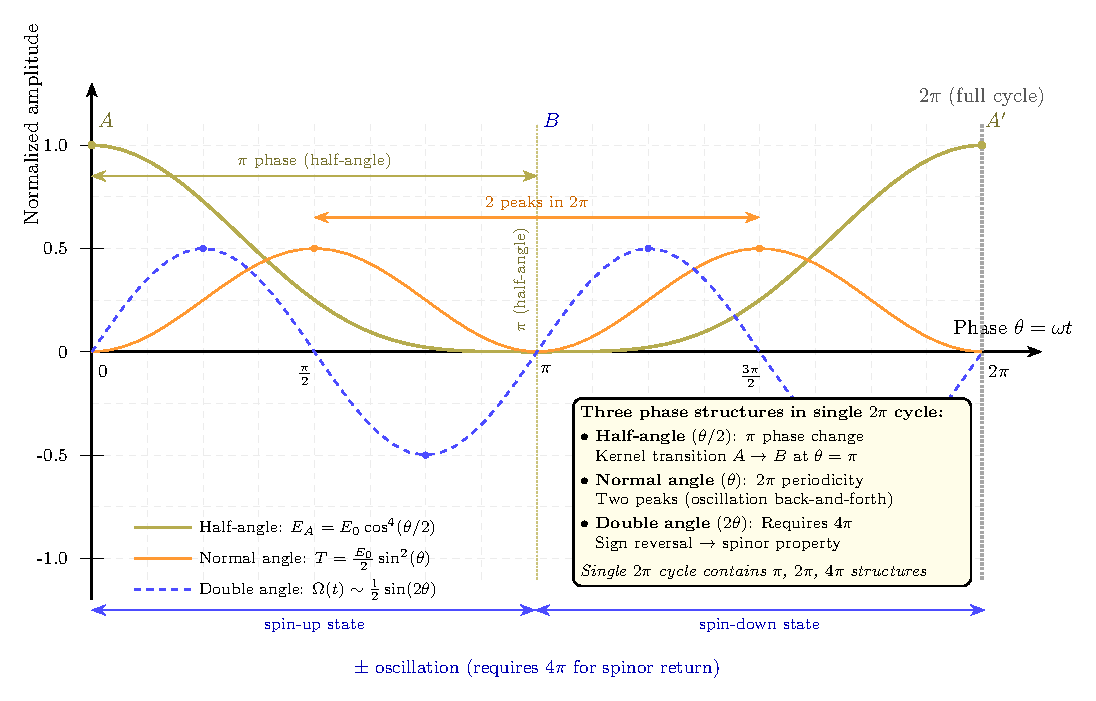
\includegraphics[width=\linewidth]{0sm_p48_fig01_three_phases.pdf}
    \caption{\textbf{Three Phase Structures Coexisting in a Single $2\pi$ Cycle.}
    Within one internal cycle $\theta: 0 \to 2\pi$, three distinct periodicities
    coexist: half-angle thermal potential energy $Te_1 \propto \cos^4(\theta/2)$ with period $\pi$
    (olive), kinetic energy of the photon sphere $T \propto \sin^2(\theta)$ with period $2\pi$
    and maximum $0.5$ (orange), and Thomas angular velocity
    $\Omega_T \propto \frac{1}{2}\sin(2\theta)$ with spinorial period $4\pi$
    and maximum $0.5$ (blue dashed; Eq.~\ref{eq:thomas_precession}).
    The common maximum value of $0.5$ in both the kinetic and Thomas curves
    reflects the structural correspondence between translational and rotational dynamics
    analyzed below (Section~\ref{sec:half_factor}).
    See text for full interpretation.}
    \label{fig:three_phases}
\end{figure*}

\begin{figure*}[t]
    \centering
    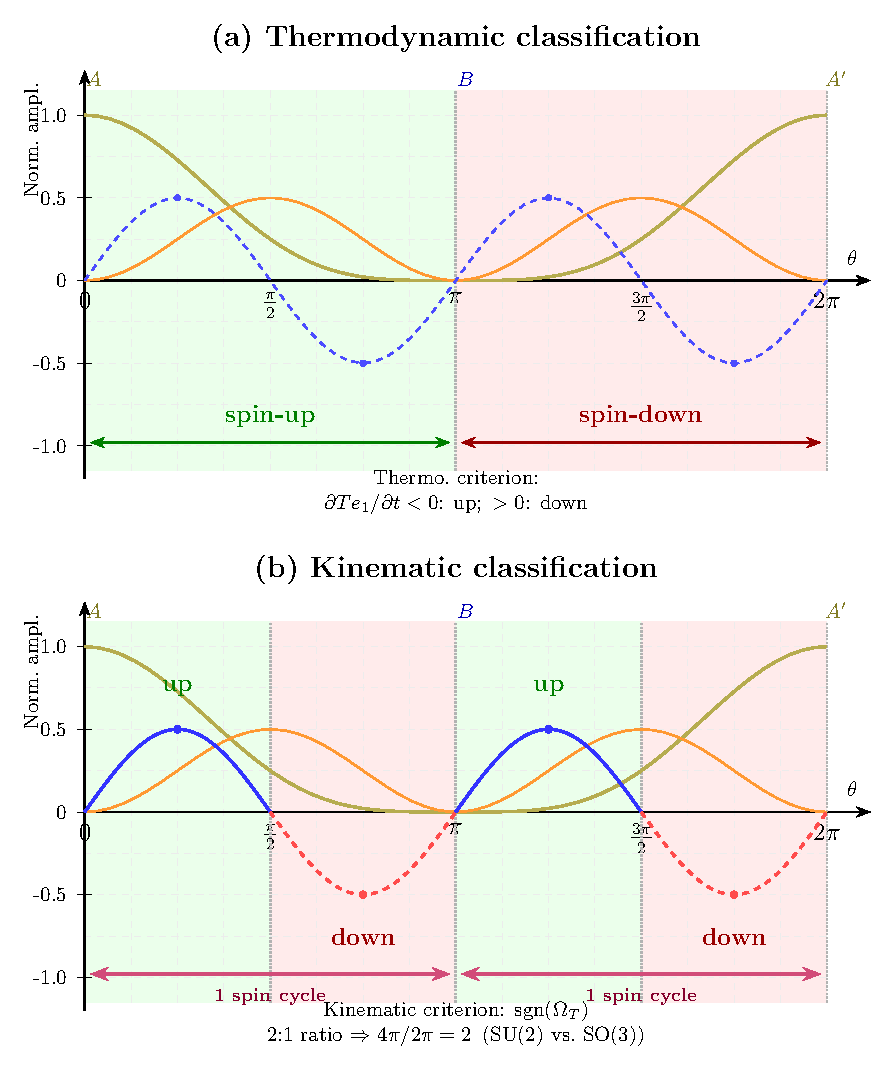
\includegraphics[width=\linewidth]{0sm_p48_fig02_two_spin_schemes.pdf}
    \caption{\textbf{Two interpretations of spin-state assignment from $\Omega_T$.}
    Both panels show the same three phase structures (olive: $E_A$;
    orange: $T$; blue/red: $\Omega_T$) over $\theta \in [0, 2\pi]$.
    \textbf{(a) Thermodynamic classification} (adopted in this paper):
    spin-up for $\theta \in [0,\pi)$ (kernel $A$ in radiation phase) and
    spin-down for $\theta \in (\pi, 2\pi]$ (absorption phase),
    preserving the Bloch sphere hemisphere identification.
    \textbf{(b) Kinematic classification} (open alternative):
    spin state assigned by $\mathrm{sgn}(\Omega_T)$, placing one complete
    up/down cycle within each kernel transit. The 2:1 frequency ratio
    directly manifests $4\pi/2\pi = 2$ (SU(2) vs.\ SO(3)).
    See text for discussion.}
    \label{fig:two_spin_schemes}
\end{figure*}

\begin{figure*}[t]
    \centering
    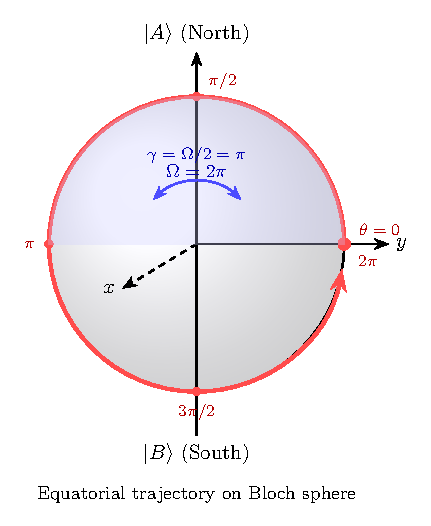
\includegraphics[width=0.5\linewidth]{0sm_p48_fig03_bloch_sphere.pdf}
    \caption{\textbf{Berry Phase from Equatorial Trajectory on Bloch Sphere}}
    \label{fig:bloch_sphere}
    \vspace{0.4em}
    \begin{minipage}{0.95\textwidth}
    \justifying\small
    Geometric representation of the internal state evolution on the Bloch sphere.
    The red trajectory traces the equatorial circle corresponding to $\theta: 0 \to 2\pi$,
    connecting the north pole $|A\rangle$ (kernel $A$) and south pole $|B\rangle$ (kernel $B$)
    via the great circle. The shaded region (blue) represents the northern hemisphere,
    subtending a solid angle $\Omega = 2\pi$ steradians.
    The Berry phase accumulated over one complete cycle is
    $\gamma_{\text{intrinsic}} = \Omega/2 = \pi$ (Eq.~\ref{eq:berry_intrinsic}),
    a consequence of the spin-$1/2$ geometric factor relating solid angle to quantum phase.
    This holonomy-protected value ensures $g_{\text{CM}} = 2$ exactly in the
    proper-time frame (Theorem~\ref{thm:g_equals_2}).
    \end{minipage}
\end{figure*}

\begin{figure*}[t]
    \centering
    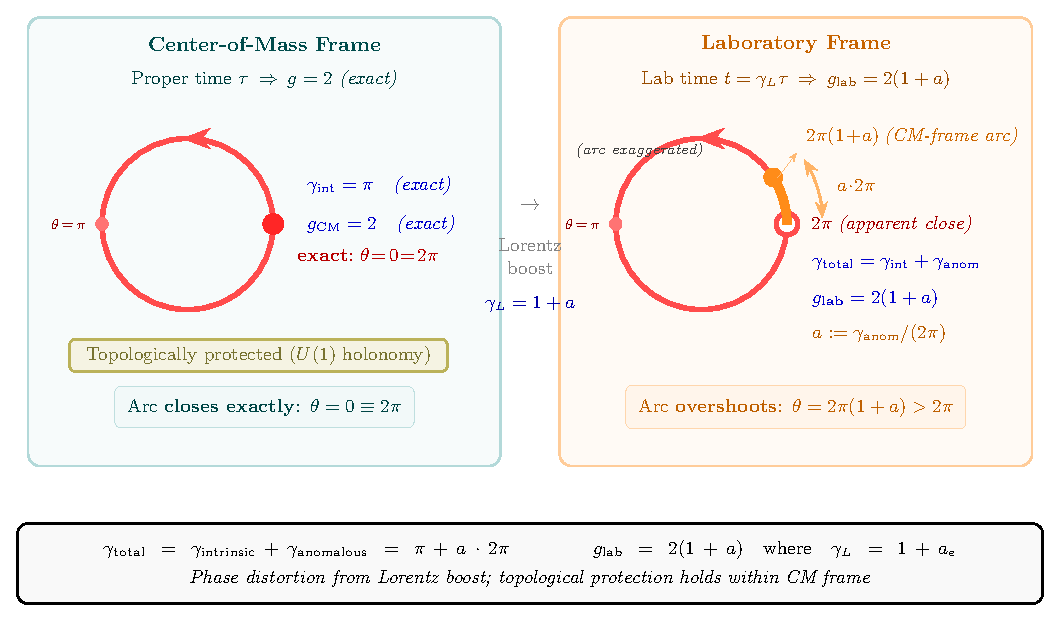
\includegraphics[width=\linewidth]{0sm_p48_fig04_dual_frame.pdf}
    \caption{\textbf{Dual Degrees of Freedom: Center-of-Mass vs.~Laboratory Frame}}
    \label{fig:dual_frame}
    \vspace{0.4em}
    \begin{minipage}{0.95\textwidth}
    \justifying\small
    Schematic illustration of the dual-frame Berry phase structure in the 0-Sphere Model.
    \textbf{Top panel (green):} In the center-of-mass frame, the internal oscillation
    evolves with proper time $\tau$, yielding intrinsic Berry phase
    $\gamma_{\text{intrinsic}} = \pi$ and $g$-factor $g_{\text{CM}} = 2$ exactly.
    This holonomy is protected against continuous deformations of the meridional path.
    \textbf{Bottom panel (orange):} Under Lorentz boost to the laboratory frame,
    time dilation ($t = \gamma_L \tau$) and relativistic effects (Thomas precession,
    Lorentz contraction) introduce a phase distortion $\delta\theta$, generating
    the anomalous Berry phase $\gamma_{\text{anomalous}}$.
    The total phase decomposes as $\gamma_{\text{total}} = \gamma_{\text{intrinsic}} + \gamma_{\text{anomalous}}$,
    yielding laboratory $g$-factor $g_{\text{lab}} = 2(1 + a)$ where
    $a := \gamma_{\text{anomalous}}/(2\pi)$ (Theorem~\ref{thm:g_lab}).
    This dual-frame structure provides a geometric framework for understanding
    the anomalous magnetic moment as a manifestation of reference frame dependence
    within Berry phase geometry.
    \end{minipage}
\end{figure*}

% ── Fig. 5: Harmonic oscillator energy ladder ────────────────
% TikZ source: 0sm_p48_fig05_zpe_ladder.tex
% Pre-compiled PDF uploaded to Overleaf as 0sm_p48_fig05_zpe_ladder.pdf
\begin{figure*}[t]
    \centering
    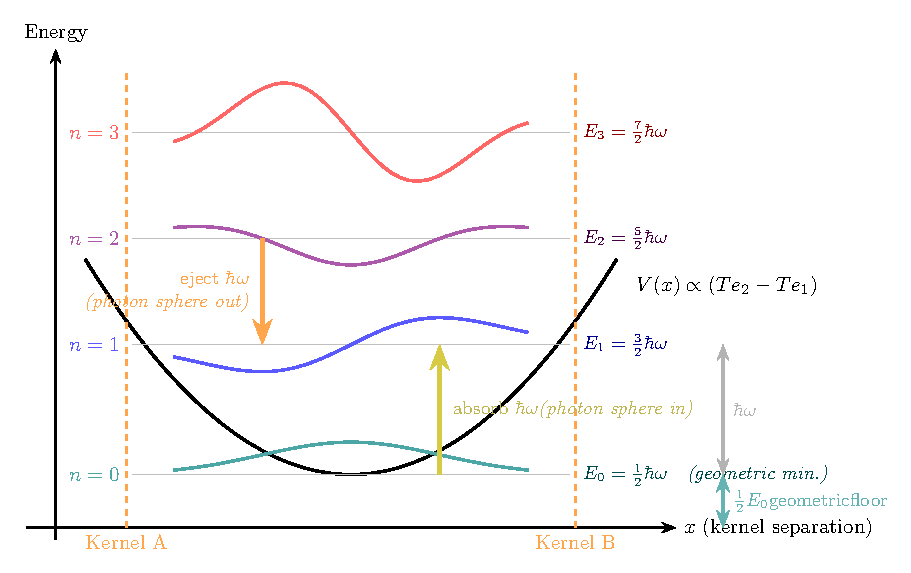
\includegraphics[width=0.80\linewidth]{0sm_p48_fig05_zpe_ladder.pdf}
    \caption{%
    \begin{minipage}[t]{0.95\textwidth}%
    \justifying
    \textbf{Harmonic oscillator energy ladder reinterpreted within
    the 0-Sphere framework.}
    The parabolic potential $V(x)$ corresponds to the effective
    confinement of the photon sphere between Kernel~A (left dashed line)
    and Kernel~B (right dashed line), separated by $\Delta x \sim \lambdaC$.
    The ground state $n=0$ with energy $\frac{1}{2}\hbar\omega$ is identified
    with the geometric minimum $E_0/2$ of the Hamiltonian identity
    (Eq.~\ref{eq:zpe_geometric})---a deterministic structural floor,
    not a probabilistic vacuum fluctuation.
    Each upward transition $n \to n+1$ corresponds to absorption of one
    photon-sphere quantum (yellow arrow);
    each downward transition $n \to n-1$ corresponds to ejection of a
    photon-sphere fragment (orange arrow).
    The ejected fragment is the microscopic mechanism underlying the
    gravitational mediator conjecture developed in the companion paper.%
    \end{minipage}}
    \label{fig:zpe_ladder}
\end{figure*}

\end{document}